% counters de propiedades, 
\newcounter{propiedad}
%
\newcounter{PropPermutacion}
\newcounter{PropBiyeccion}
\newcounter{PropCotamaxima}
\newcounter{PropConcavidad}
\newcounter{PropSchurConcavidad}
\newcounter{PropRecursividad}
\newcounter{PropCadena}
\newcounter{PropIndependenciaCondicional}
%
%
% propiedades generales
\newenvironment{propiedades}
{\begin{enumerate}[label={[P\arabic*]}]\setcounter{enumi}{\value{propiedad}}}
{\setcounter{propiedad}{\value{enumi}}\end{enumerate}}
%
% propiedades cambiadas en el caso continuo
\newenvironment{propiedadesC}
{\begin{enumerate}[label={[P'\arabic*]}]}
{\end{enumerate}}
%
% propiedades cambiadas en el caso de (h,phi)-entropias
\newenvironment{propiedadesPhi}
{\begin{enumerate}[label={[P$_\phi$\arabic*]}]}
{\end{enumerate}}


% Ber74 => ensemble de papiers clés sur la theorie du codage

%%%%%%%%%%%%%%%%%%%%%%%%%%%%%%%%%%%%%%%%%%%%%%%%%%%%%%%%%%%%%%%%%%%%%%%%%%%%%%%

\capitulo{Nociones de teor\'ia de la informaci\'on}{}
%Steeve Zozor}
\label{Cap:SZ:Informacion}

% Epigrafe de capitulo
\begin{epigrafe}
%``Mi   preocupación  más   grande  era   cómo  llamarla.   Pensé  en   llamarla
%‘información’,  pero esa  palabra estaba  muy usada,  de forma  tal que  decidí
%llamarla ‘incerteza’.  Cuando discutí el asunto  con John von Neumann,  el tuvo
%una idea mejor. Von Neumann me dijo:
  ``Deber\'ias llamarla `entrop\'ia', por dos motivos.\\
  En  primer  lugar  su funci\'on  de  incerteza\\
  ha  sido  usada en  la  mec\'anica  estad\'istica\\
  bajo ese nombre, y por ello, ya tiene un nombre.\\
  En segundo lugar,  y lo que  es m\'as importante,\\
  nadie sabe  lo que es realmente la entrop\'ia,\\
  por ello, en un debate, siempre llevar\'as la ventaja.
%  ``You should call it entropy, for two reasons.\\
%  In the first place your  uncertainty function\\
%  has been used  in statistical mechanics\\
%  under that  name, so it already  has a name.\\
%  In the  second place, and more  important,\\
%  no one knows what entropy really is,\\
%  so in a  debate you will always have  the advantage''
  %
  \autortituloepigrafe{J. von Neumann to C. Shannon~\cite{TriMcI71}}
\end{epigrafe}

\minitoc


% =============================== Introduccion =============================== %


\seccion{Introducci\'on}
\label{s:SZ:Introduccion}

La  noci\'on  de  informaci\'on encuentra  su  origen  con  el desarollo  de  la
comunicaci\'on  moderna,  por ejemplo  a  trav\'es  del  telegrafo siguiendo  el
patente de Moorse  en 1840. La idea  de asignar un c\'odigo (punto  o barra, mas
espacio entre letras  y entre palabras) a las letras del  alfabeto es la semilla
de  la  codificaci\'on   entropica,  la  que  se  basa   precisamente  sobre  la
asignaci\'on de un c\'odigo a  simbolos de una fuente (codificaci\'on de fuente)
seg\'un las frequencias  (o probabilidad de aparici\'on) de  cada simbolo en una
cadena.  De  hecho, el principio de  codificar un mensage y  mandar la versi\'on
codificada por un canal de transmisi\'on es mucho mas antiguo, a pesar de que no
habia ninguna formalizaci\'on matematica ni siquiera explicitamente una noci\'on
de informaci\'on.  Entre otros, se puede mencionar el telegrafo optico de Claude
Chappe (1794), experimentos con luces por Guillaume Amontons (en los a\~nos 1690
en Paris), o a\'un mas antiguamente la transmisi\'on de mensaje con antorchas en
la   Grecia   antigua,   con  humo   por   los   indios   o  chiflando   en   la
prehistoria~\cite{Mon08}.  Cada  forma es una instancia practica  del esquema de
comunicaci\'on de Shannon~\cite{Sha48, ShaWea64},  es decir la codificaci\'on de
la informaci\'on,  potencialmente de  manera la mas  economica que se  puede, su
transmisi\'on   a   un   ``receptor''    (por   un   canal   ruidoso)   que   la
interpreta/lee/decodifica.   Implicitamente, la noci\'on  de informaci\'on  a lo
menos tan antigua que la humanidad.

A  pesar  de  que  la  idea  de codificar  y  transmitir  ``informaci\'on''  sea
tremendamente antigua, la formalizaci\'on matematica de la noci\'on de incerteza
o falta de informaci\'on, intimamente  vinculado a la noci\'on de informaci\'on,
naci\'o bajo el  impulso de C.  Shannon y la publicaci\'on  de su papel seminal,
``A  mathematical theory  of communication''  en 1948~\cite{Sha48},  o  un a\~no
depues  en su  libre re-titulado  ``The mathematical  theory  of communication''
reamplanzando el ``A'' por un ``The''. Desde esto a\~nos, las herramientas de la
dicha teoria de  la informaci\'on dio lugar a  muchas aplicaciones especialmente
en communicaci\'on (ver por  ejemplo~\cite[y ref.]{CovTho06, Ver98, Gal01}, pero
tambi\'en en otros campos muy diversos tal como \SZ{Completar con ref, Boltzman,
  von Neumann, Gibbs, Maxwell, Planck\ldots}.

{\color{red} La  meta de este cap\'itulo es  de describir las ideas  y los pasos
  dando lugar a la definicion de  la entropia, como medida de incerteza o (falta
  de)  informaci\'on.   En este  cap\'itulo,  se  empieza  con la  descripci\'on
  intuitiva que subtiende a la noci\'on de informaci\'on contenida en una cadena
  de simobolo, lo que condujo a  la definici\'on de la entropia. Esta defici\'on
  puede  ser deducida  tambi\'en  de  una seria  de  propiedades razonables  que
  deber\'ia cumplir  una medida de incerteza (enfoque  axiomatico).  Se continua
  con la descripci\'on  de tal noci\'on de entropia,  pasando del mundo discreto
  (simbolos,  alfabeta) al  mundo continuo,  lo que  no es  trivial  ni siquiera
  intuitivo.  Se  adelanto presentando  el concepto de  informaci\'on compartida
  entre dos sistemas o variables aleatorias, concepto fundamental en el marco de
  la transmisi\'on de informaci\'on o de mensajes. \bf Seguir. }


% ================================= Entropia ================================= %

\seccion{Entrop\'ia como medida de incerteza}
\label{s:SZ:Entropia}

% ================================= Axiomas

\subseccion{Entrop\'ia de Shannon, propiedades}
\label{sec:SZ:DefinicionShannon}

Un de los primeros trabajos  tratando de formalizar la noci\'on de informaci\'on
de una cadena  de simbolos es debido a Raph  Hartley~\cite{Har28}.  En su papel,
Hartley defin\'o la informaci\'on de una secuencia como siendo proporcional a su
longitud. Mas precisamente,  para simbolos de un alfabeto  de cardinal $\alpha$,
exiten  $\alpha^n$   cadenas  diferentes  de   longitud  $n$;  Se   defin\'o  la
informaci\'on de tales cadenas como  siendo $K n$ ($K$ dependiente de $\alpha$).
Para  ser  consistente,  dos   conjuntos  de  mismo  tamanio  $\alpha_1^{n_1}  =
\alpha_2^{n_2}$   deben  llegar  a   la  misma   informaci\'on,  as\'i   que  la
informaci\'on de Hartley es definida como $H = \log\left( \alpha^n \right)$ donde
la base del logaritmo es arbitraria.  Dicho de otra manera, tomando un logaritmo
de  base 2,  esta  informaci\'on  es nada  mas  que los  numeros  de bits  (0-1)
necesarios para  codificar todas las cadenas  de longitud $n$ de  simbolos de un
alfabeto de cardinal $\alpha$.

\SZ{Hartley, equiv de Gibbs de la termostat}.

Una debilidad del  enfoque de Hartley es que considera  implicitamente que en un
mensage, cada cadena de longitud dada  puede aparecer con la misma frecuencia, o
probabilidad $1/\alpha^n$,  siendo la informaci\'on menos el  logaritmo de estas
probabilidades.  A contrario, parece  mas l\'ogico considerar que secuencias muy
frecuentes no  llevan mucha informaci\'on  (se sabe que aparecen),  mientras que
las  que aparencen  raramente llevan  mas informaci\'on  (hay mas  sorpresa, mas
incerteza  en observarlas).  Volviendo  a los  simbolos elementales  $x$, vistos
como aleatorios (o valores o estados que puede tomar una variable aleatoria), la
(falta  de)  informaci\'on o  incerteza  va a  ser  intimamente  vinculada a  la
probabilidad de aparici\'on de estos simbolos $x$. Siguiendo la idea de Hartley,
la informaci\'on elemental  asociado al estado $x$ va a ser  $- \log p(x)$ donde
$p(x)$  es la  probabilidad de  apararici\'on de  $x$.  Se  define  la incerteza
asociada a  la variable aleatoria como  el promedio estadistico  sobre todos los
estados  posibles $x$~\cite{Sha48, ShaWea64}~\footnote{En  la misma  \'epoca que
  Shannon,  independientemente,   la  noci\'on  de   informaci\'on  o  medidades
  equivalentes apareciendo por ejemplo en calculo de capacidad de canal aparecen
  en  varios  trabajo  como  el de  Calvier~\cite{Cla48},  Laplume~\cite{Lap48},
  Wiener~\cite[Cap.~III]{Wie48}  entre  varios  otros  (ver~\cite{Ver98,  Lun02,
    RioMag14, FlaRio16, RioFla17, Che17}).}.
%
% \cite{Sha48, ShaWea64}
\begin{definicion}[Entropia de Shannon]\label{def:SZ:Shannon}
  Sea $X$ una variable aleatoria definida  sobre una alpfabeto discreto $\X = \{
  x_1 , \ldots , x_\alpha \}$ de cardinal $\alpha = |\X| < + \infty$ finito. Sea
  $p_X$ la  distribuci\'on de probabilidad  de $X$, \ie  $ \forall \, x  \in \X,
  \quad p_X(x)  = \Pr[X  = x]$.  La entropia de  Shannon de  la variable  $X$ es
  definida por
  %
  \[
    H(p_X) = H(X) = - \sum_{x \in \X} p_X(x) \, \log p_X(x)
  \]
  %
  con la convenci\'on $0 \log 0 = 0$.
\end{definicion}

La base del logaritmo es arbitrario; si  es $\log_2$ el logaritmo de base 2, $H$
es en bits y si se usa el logaritmo natural $\ln$, $H$ es en nats.  {\it En este
  cap\'itulo, se usara  $H$ con el logaritmo correspondiente  sin especificar la
  base.  Si  es necesario  que tenga  una base $a  (\ne 1)$  dada, se  notara la
  entropia  corespondiente  $H_a$  y   se  especifiera  la  base  del  logaritmo
  $\log_a$}.  Fijense de que $\log_a x = \frac{\log x}{\log a}$, dando
%
\[
H_a(X)  =  H_b(X)  \log_a b
\]
%
En  lo  que  sigue, a\'un  que,  rigorosamente,  $H$  sea  una funci\'on  de  la
distribuci\'on  de  probabilidad  $p_X$  y  no  de la  variable  $X$,  se  usara
indistamente la notaci\'on $H(p_X)$ tal  como $H(X)$ seg\'un lo mas conveniente.
Ademas, $p_X$ podr\'a denotar  indistamente la distribuci\'on de probabilidad, o
el  vector  de probabilidad  $p_X  \equiv  \begin{bmatrix}  p_X(x_1) &  \cdots  &
  p_X(x_\alpha) \end{bmatrix}^t$.

$H$ tiene propiedades notables, que coresponden a las que se puede exigir de una
medida de incerteza~\cite{Sha48, ShaWea64, CovTho06, Rio07, DemCov91, Joh04}:
%
\begin{propiedades}
\item\label{prop:SZ:continuidad} {\it Continuidad:}  Vista como una funci\'on de
  \ $\alpha$ \ variables  \ $p_i = p_X(x_i)$, \ $H$ \  es continua con respeto a
  los $p_i$.
%
\setcounter{PropPermutacion}{\value{enumi}}
\item\label{prop:SZ:permutacion}   {\it  Invariance  bajo   una  permutaci\'on:}
  Obviamente,  la   entropia  es  invariante  bajo  una   permutaci\'on  de  las
  probabilidades, \ie,
  %
  \[
  \mbox{para cualquier  permutaci\'on } \sigma:  \X \to \X, \quad  H(p_{\sigma(X)}) =
  H(p_X) \quad \mbox{con} \quad p_{\sigma(X)}(x) = p_X(\sigma(x))
  \]
  %
  lo que se  escribe tambi\'en $H(\sigma(X)) = H(X)$.   En particular, denotando
  $p_X^\downarrow$ la  distribuci\'on de probabilidades obtenida a  partir de $p_X$,
  clasificando las  probabilidades en orden  decreciente, $p_X^\downarrow(x_1) \ge
  p_X^\downarrow(x_2) \ge \cdots  \ge p_X^\downarrow(x_\alpha)$,
  %
  \[
  H(p_X^\downarrow) = H(p_X)
  \]
%
\setcounter{PropBiyeccion}{\value{enumi}}
\item\label{prop:SZ:biyeccion}   {\it  Invariance   bajo   una  transformaci\'on
    biyectiva:}  La  entropia  es  invariante  bajo  cualquier  transformaci\'on
  biyectiva, \ie
  %
  \[
  \mbox{para cualquier  funci\'on biyectiva } g:  \X \to g(\X),  \quad H(g(X)) =
  H(X)
  \]
  %
  A  trav\'es  tal transformaci\'on  los  estados  cambian,  pero no  cambia  la
  distribuci\'on de probabilidad vinculada al alfabeto transformado.  Tomando el
  ejemplo de  un dado, la  incerteza vinculada al  dado no debe depender  de los
  simbolos escritos sobre las caras, sean enteras o cualquier letras.
%
\item\label{prop:SZ:positividad} {\it  Positividad:} La entropia  es acotada por
  debajo,
  %
  \[
  H(X) \ge 0 
  \]
  %
  con iguladad si y solamente si existe un $x_0 \in \X$ tal que $p_X(x_0) = 1$ \
  y \  $p_X(x) = 0$ \ para  \ $x \ne x_0$,
  %
  \[
  H(X)  =  0 \quad  \mbox{ssi}  \quad X  \mbox{  es  deterministico}
  \]
  %
  En  otras  palabras, cuando  $X$  no  es aleatoria,  \ie  $X  =  x_0$, no  hay
  incerteza, o  la observaci\'on  no lleva  informaci\'on (se sabe  lo que  va a
  salir, sin duda): $H = 0$.   La positividad es consecuencia de $p_X(x) \le 1$,
  dando $- p_X(x)  \log p_X(x) \ge 0$.  Ademas, la suma  de terminos positive es
  cero si y solo si  cada termino es cero, dando \ $p_X(x) = 0$  \ o \ $p_X(x) =
  1$.
%
\setcounter{PropCotamaxima}{\value{enumi}}
\item\label{prop:SZ:cotamaxima}  {\it Maximalidad:} La  entropia es  acotada por
  arriba,
  %
  \[
  H(X) \le \log \alpha
  \]
  %
  con iguladad si y solamente si existe $X$ es uniforme sobre $\X$, \ie
  %
  \[
  H(X) =  \log \alpha \quad \mbox{ssi}  \quad \forall \,  x \in \X, \:  p_X(x) =
  \frac{1}{\alpha}
  \]
  %
  En otras  palabras, la incerteza es  maxima cuando cualquier  estado $x$ puede
  aparecer con la misma probabilidad; cada observaci\'on lleva una informaci\'on
  importante sobre el  sistema que genera $X$.  La cota  m\'axima resuelta de la
  maximisaci\'on de $H$  sujeto a $\sum_x p_X(x) = 1$, es  decir, con la tecnica
  del Lagrangiano, notando $p_i =  p_X(x_i)$, de la minimizaci\'on de $\sum_i (-
  p_i  \log p_i  + \lambda  p_i)$.   Se obtiene  sencillamente que  $\log p_i  =
  -\lambda$,      dando     la      distribuci\'on      uniforma.\newline     La
  figura~\ref{fig:SZ:EntropiaBinaria} representa la entropia de un sistema a dos
  estados, de probabilidades  \ $\lambda$ \ y \ $1-\lambda$  \ (lei de Bernoulli
  de parametro  $\lambda$), entropia  a veces dicha  {\it entropia  binaria}, en
  funci\'on de $\lambda$.   Esta figura ilustra ambas cotas ($\lambda  = 1$ o 1,
  $\lambda  =  \frac12$)  as\'i   que  la  invariancia  bajo  una  permutaci\'on
  ($h(\lambda) = H(\lambda,1-\lambda) = H(1-\lambda,\lambda) = h(1-\lambda)$).
  %
  \begin{figure}[h!]
  %
  \begin{center}\begin{tikzpicture}
\shorthandoff{>}
%
% Entropia binaria
\begin{scope}[xscale=3.5,yscale=2.5]
%
\draw[>=stealth,->] (-.05,0)--(1.15,0) node[right]{\small $r$};
\draw[>=stealth,->] (0,-.05)--(0,1.1) node[above]{\small $h(r)$};
\draw[thick,domain=.01:.99,samples=200] (0,0)-- plot (\x,{-\x*log2(\x)-(1-\x)*log2(1-\x)}) --(1,0);
\draw (0,0)--(0,-.02) node[below]{\small $0$};
\draw (1,0)--(1,-.02) node[below]{\small $1$};
\draw (0,1)--(-.02,1) node[left]{\small $\log 2$};
\end{scope}
\end{tikzpicture}\end{center}
  %
  \leyenda{Entropia  binaria  (de  una  variable  de  Bernoulli)  $h(\lambda)  =
    H(\lambda,1-\lambda)$ en funci\'on de $\lambda \in [0 , 1]$.}
  %
  \label{fig:SZ:EntropiaBinaria}
  \end{figure}
%
\item\label{prop:SZ:expansabilidad} {\it Expansibilidad:}  A\~nadir un estado de
  probabilidad 0 no cambia la entropia, \ie sean \ $X$ \ definido sobre \ $\X$ \
  y \ $\widetilde{X}$ \ sobre \ $\widetilde{X}$,
  %
  \[
  \widetilde{\X}  =  \X  \cup  \{  \widetilde{x}_0  \}  \quad  \mbox{con}  \quad
  p_{\widetilde{X}}(x)   =   p_X(x)   \quad   \mbox{si}   \quad  x   \in   \X,   \quad
  p_{\widetilde{X}}(\widetilde{x}_0)    =    0,    \qquad   \mbox{entonces}    \quad
  H(p_{\widetilde{X}}) = H(p_X)
  \]
  %
  Esta propiedad es obvia, consecuencia de $\lim_{p \to 0} p \log p = 0$.
%
\setcounter{PropRecursividad}{\value{enumi}}
\item\label{prop:SZ:recursividad} {\it Recursividad:} Juntar dos estados baja la
  entropia de una cantidad igual a la entropia interna de los dos estados por la
  probabilidad de ocurencia de este  conjunto de estados, y vice-versa, \ie sean
  \ $X$ \ definido sobre \ $\X$ \ y \ $\overline{X}$ \ sobre \ $\overline{X}$,
  %
  \[
  \left\{  \begin{array}{l}\overline{\X} =  \{  x_1 ,  \ldots  , x_{\alpha-2}  ,
      \overline{x}_{\alpha-1}\}  \quad   \mbox{con  el  estado   interno}  \quad
      \overline{x}_{\alpha-1}   =  \{   x_{\alpha-1}  ,   x_\alpha  \},\\[2.5mm]
      p_{\overline{X}}(x_i)  = p_X(x_i),  \quad 1  \le i  \le \alpha-1  \quad \mbox{y}
      \quad p_{\overline{X}}(\overline{x}_{\alpha-1}) = p_X(x_{\alpha-1}) +
      p(x_\alpha)  \quad  \mbox{distribuci\'on  sobre  }  \overline{\X}\\[2.5mm]
      \displaystyle   \overline{q}(x_j)    =   \frac{p_X(x_j)}{p_X(x_{\alpha-1})   +
        p_X(x_\alpha)}, \quad j =  \alpha-1, \alpha \quad \mbox{distribuci\'on del
        estado   interno}\end{array}\right.
  \]
  %
  \[
  H(p_X)  = H(p_{\overline{X}})  +  p_{\overline{X}}(\overline{x}_{\alpha-1}) \,
  H(\overline{q})
  \]
  %
  Esta relaci\'on  viene de $a \log  a + b  \log b = (a+b)  \left( \frac{a}{a+b}
    \log\left(  \frac{a}{a+b} \right)  + \frac{b}{a+b}  \log\left( \frac{a}{a+b}
    \right)   -    \log(   a    +   b   )\right)$    esta   ilustrada    en   la
  figura~\ref{fig:SZ:Recursividad} siguiente.\newline
  %
  \begin{figure}[h!]
  %
  \begin{center} %\hskip 2.5cm
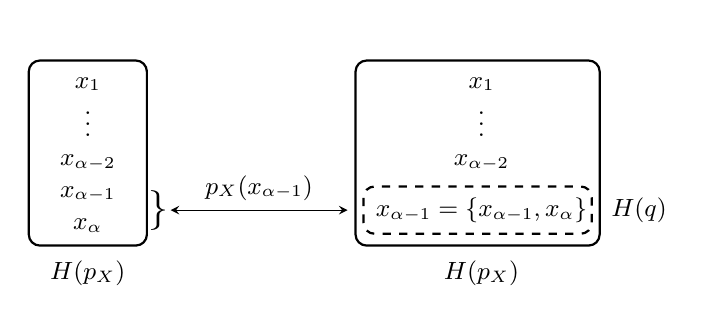
\begin{tikzpicture}
\shorthandoff{>}
%
% Ensemble \X
\draw(0,3) node{\small $\X$};
\draw(0,2.4) node{\small $x_1$};
\draw(0,2) node{\small $\vdots$};
\draw(0,1.4) node{\small $x_{\alpha-2}$};
\draw(0,1) node{\small $x_{\alpha-1}$};
\draw(0,.6) node{\small $x_{\alpha}$};
\draw(0,0) node{\small $H(p_X)$};
\draw[thick,rounded corners] (-.75,.35) rectangle (.75,2.7);
%
% Ensemble \widebar{\X}
%
\draw(5,3) node{\small $\widebar{\X}$};
\draw(5,2.4) node{\small $x_1$};
\draw(5,2) node{\small $\vdots$};
\draw(5,1.4) node{\small $x_{\alpha-2}$};
\draw(5,.8) node{\small $\widebar{x}_{\alpha-1} = \{ x_{\alpha-1} , x_\alpha\}$};
\draw(5,0) node{\small $H(p_{\widebar{X}})$};
\draw(7,.8) node{\small $H(\widebar{q})$};
\draw[dashed,thick,rounded corners] (3.5,.5) rectangle (6.4,1.1);
\draw[thick,rounded corners] (3.4,.35) rectangle (6.5,2.7);
%
% juntando 2 estados VER PROBLEMA CON LA FLECHA
\draw(.9,.8) node{\Large $\}$};
\draw[>=stealth,<->] (1.05,.8)--(3.3,.8);
\draw (2.175,.8) node[above]{\small $p_{\widebar{X}}(\widebar{x}_{\alpha-1})$};
\end{tikzpicture} \end{center}
  %
  \leyenda{Ilustraci\'on de  la propiedad  de recursividad, que  cuantifica como
    decrece la entropia en un  conjunto cuando se juntan dos estados, vincluando
    la entropia  total, la  entropia despues del  la agrupaci\'on y  la entropia
    interna a los dos estados juntados.}
  %
  \label{fig:SZ:Recursividad}
  \end{figure}
%
\setcounter{PropConcavidad}{\value{enumi}}
\item\label{prop:SZ:concavidad} {\it Concavidad:} La  entropia es concava, en el
  sentido  de que  la entropia  de una  combinaci\'on convexa  de distribuciones
  (mezcla) de probabilidades es siempre major o igual a la combinaci\'on convexa
  de entropias:
  %
  \[
  \forall \: \{ \lambda_i \}_{i=1}^n, \quad  0 \le \lambda_i \le 1, \quad \sum_i
  \lambda_i = 1  \quad \mbox{and cualquier conjunto de  distribuciones} \quad \{
  p_i \}_{i=1}^n,
  \]
  %
  \[
  H\left(  \sum_i  \lambda_i p_i  \right)  \ge  \sum_i  \lambda_i H(p_i)
  \]
  %
  Esta desigualdad es conocida como  desigualdad de Jensen.  Es una consequencia
  directa de  la convexidad  de la funci\'on  $\phi: u  \mapsto u \log  u$, como
  ilustrado       en       la      figura~\ref{fig:SZ:Concavidad}-(a).        La
  figura~\ref{fig:SZ:Concavidad}-(b) ilustra como se puede obtener una mezcla de
  distribuciones  de  dos probabilidad  $p_1$  (dado  izquierda)  y $p_2$  (dado
  derecho)  haciendo una elecci\'on  aleatoria a  partir de  una moneda  en este
  ejemplo (probabilidad $\lambda$ de elegir el dado izquierda).\newline
  %
  \begin{figure}[h!]
  %
  \begin{center} \begin{tikzpicture}
\shorthandoff{>}
%
% Concavidad de - u log u
\begin{scope}[xscale=3,yscale=2.5]
\pgfmathsetmacro{\u}{.2};
\pgfmathsetmacro{\v}{1.25};
\pgfmathsetmacro{\l}{.7};
%
\draw[>=stealth,->] (-.5,0)--(1.6,0) node[right]{\small $u$};
\draw[>=stealth,->] (0,-.7)--(0,{1.5*log2(1.5)}) node[above]{\small $\phi(u) = u \log u$};
\draw[thick,domain=.005:1.5,samples=200] (0,0)-- plot (\x,{\x*log2(\x)});
\draw[dashed] (\u,{\u*log2(\u)})--(\v,{\v*log2(\v)});
\draw (\u,0)--(\u,-.05) node[below]{\small $u_1$};
\draw (\v,0)--(\v,-.05) node[below]{\small $u_2$};
%
\draw[dashed] ({\l*\u+(1-\l)*\v},.05) node[above]{\small $\lambda u_1 + (1-\lambda) u_2$}
--({\l*\u+(1-\l)*\v},{(\l*\u+(1-\l)*\v)*log2(\l*\u+(1-\l)*\v)});
%
% l phi(u) + (1-l) phi(v)
\draw[dotted]
({\l*\u+(1-\l)*\v},{\l*\u*log2(\u)+(1-\l)*\v*log2(\v)})--(-.05,{\l*\u*log2(\u)+(1-\l)*\v*log2(\v)})
node[left]{\small $\lambda \phi(u_1) + (1-\lambda) \phi(u_2)$};
%
% phi(l u + (1-l) v)
\draw[dotted]
({\l*\u+(1-\l)*\v},{(\l*\u+(1-\l)*\v)*log2(\l*\u+(1-\l)*\v)})--
(-.05,{(\l*\u+(1-\l)*\v)*log2(\l*\u+(1-\l)*\v)})
node[left]{\small $\phi(\lambda u_1 + (1-\lambda) u_2)$};
\end{scope}
%
%
% Concavidad / mezcla
\begin{scope}[xshift=8.5cm]
\draw(0,1.25) node{\includegraphics[width=3cm]{TIKZ_SZ/DosDados}};
\draw(-.5,2.5) node{\small $p_1$};
\draw(1,2) node{\small $p_2$};
\draw(2.7,1) node{\small $\lambda p_1 + (1-\lambda) p_2$};
\draw(-.25,-1) node{\includegraphics[width=1cm]{TIKZ_SZ/Moneda}};
\draw[>=stealth,->,thick] (-.3,-.35)--(-.75,.45);
\draw (-.525,0) node[left]{\small $\lambda$};
\draw[>=stealth,->,thick] (-.2,-.35)--(.3,.45);
\draw (.05,0) node[right]{\small $1-\lambda$};
\end{scope}
%
\draw (1.25,-2.25) node{(a)};
\draw (8.25,-2.25) node{(b)};
\end{tikzpicture} \end{center}
  %
  \leyenda{(a) $\phi(u)  = u \log u$ es  convexa: la curva es  siempre debajo de
    sus cuerdas; entonces, cada promedio de $\phi(u_1)$ y $\phi(u_2)$ estando en
    la cuerda  juntando estos punto, queda  arriba de la funci\'on  tomada en el
    promedio de $u_1$  y $u_2$.  Escribiendo eso para (mas  de dos puntos) sobre
    los $\sum_i \lambda_i  p_i(x)$ y sumando sobre los $x$  da la desigualdad de
    Jensen.  (b) Ilustraci\'on de  una distribuci\'on de mezcla, ac\'a mezclando
    $p_1$  y  $p_2$  a  partir  de  una tercera  variable  aleatoria  (ac\'a  de
    Bernoulli).}
  %
  \label{fig:SZ:Concavidad}
  \end{figure}
%
\setcounter{PropSchurConcavidad}{\value{enumi}}
\item\label{prop:SZ:Schurconcavidad}  {\it Schur-concavidad:}  Como se  lo puede
  querrer,  lo mas  ``concentrado'' es  una distribuci\'on  de  probabilidad, lo
  menos hay  incerteza, y entonces lo  mas peque\~no debe ser  la entropia. Esta
  propiedad intuitiva se resuma a partir de la noci\'on de mayorizaci\'on:
  %
  \begin{definicion}[Mayorizaci\'on]\label{def:SZ:Mayorizacion}
    Una distribuci\'on  discreta finita de probabilidad $p$  es dicha mayorizada
    por una distribuci\'on $q$,
    %
    \[
    p  \prec  q  \quad   \mbox{ssi}  \quad  \sum_{i=1}^k  p^\downarrow(x_i)  \le
    \sum_{i=1}^k q^\downarrow(x_i), \quad 1 \le  k < \alpha \quad \mbox{y} \quad
    \sum_{i=1}^\alpha p^\downarrow(x_i)  = \sum_{i=1}^\alpha q^\downarrow(x_i)
    \]
    %
    (las \'ultimas sumas siendo igual a 1).  Si los alfabetos de definici\'on de
    \ $p$ \ y  \ $q$ \ son de tama\~nos diferentes, \  $\alpha$ \ es el tama\~no
    lo  mas  grande y  la  distribuci\'on  sobre el  alfabeto  lo  mas corto  es
    completada por estados de probabilidad 0 (recuerdense de que no va a cambiar
    la entropia).
  \end{definicion}
  %
  La  Schur-concavidad  se  traduce  por  la  relaci\'on
  %
  \[
  p \prec  q \quad \Rightarrow  \quad H(p) \ge  H(q)
  \]
  %
  Fijense de que las cotas sobre $H$ pueden ser vistas como consecuencia de esta
  desiguldad:  la  distribuci\'on  cierta  mayoriza cualquier  distribuci\'on  y
  cualquier  distribuci\'on   mayoriza  la  distribuci\'on  uniforme~\cite[p.~9,
  (6)-(8)]{MarOlk11}.  Ademas, de la Schur-concavidad se obtiene
  %
  \[
  H\left( \begin{bmatrix}  \frac1\alpha & \cdots  & \frac1\alpha \end{bmatrix}^t
  \right) \quad \mbox{es una funci\'on creciente de } \alpha
  \]
  %
  La prueba  de la Schur-concavidad  se apoya sobre  la desigualdad de  Schur (o
  Hardy-Littlewood-P\'olya    o    Karamata)~\cite{Sch23,    HarLit29,    Kar32,
    HarLit52},~\cite[Cap.~3,                                 Prop.~C.1]{MarOlk11}
  o~\cite[Teorema~II.3.1]{Bha97}: $p \prec q  \: \Rightarrow \: \sum_i \phi(p_i)
  \le  \sum_i  \phi(q_i)$  para  cualquier  funci\'on  $\phi$  convexa.   Sufice
  considerar $\phi(u) = u \log u$ para concluir.
\end{propiedades}
%
% Ver Schur-Ostrowski f  sym, Scur-convexe ssi (xi - xj)  (df/dx_i - df/dxj) \ge
% 0, 1 \le i \ne j \le alpha


En muchos  casos, uno tiene que  trabajar con varias  variables aleatorias. Para
simplificar les  notaciones, considera una par  de variables \  $X$ \ y \  $Y$ \
definidas respectivamente sobre los alfabetos \ $\X$  \ y \ $\Y$ \ de cardinal \
$\alpha = |\X|$ \ y \ $\beta =  |\Y|$.  Tal par de variable puede ser vista como
una  variable $(X,Y)$  definida sobre  el alfabeto  $\X \times  \Y$  de cardinal
$\alpha \beta$ tal  que se definie naturalmente la  entropia para esta variable;
tal entropia es llamada {\it entropia conjunta} de $X$ y $Y$:
%
%~\cite{Sha48, ShaWea64}
\begin{definicion}[Entropia conjunta]\label{def:SZ:EntropiaConjunta}
  Sean \ $X$ \ e \ $Y$  \ dos variable aleatorias definidas sobre los alpfabetos
  discretos \  $\X$ \ y \ $\Y$,  de cardinal \ $\alpha  = |\X| < +\infty$  \ y \
  $\beta  =   |\Y|  <  +\infty$  \   respectivamente.  Sea  \   $p_{X,Y}$  \  la
  distribuci\'on de probabilidad conjunta de \ $X$ \ e \ $Y$, \ \ie $ \forall \,
  (x,y) \in \X \times \Y, \quad p_{X,Y}(x,y) =  \Pr[X = x , Y = y]$. La entropia
  conjunta de Shannon de las variables \ $X$ \ e \ $Y$ \ es definida por
  %
  \[
  H(p_{X,Y}) =  H(X,Y) = -  \sum_{(x,y) \in \X  \times \Y} p_{X,Y}(x,y)  \, \log
  p_{X,Y}(x,y)
  \]
  %
  con la convenci\'on $0 \log 0 = 0$.
\end{definicion}

A partir de esta definici\'on,  aparecen otras propiedades importantes, sino que
fundamentales, de la entropia de Shannon.
%
\begin{propiedades}
\item\label{prop:SZ:aditividad}  {\it Aditividad:} La  entropia conjunta  de dos
  variables aleatorias  \ $X$  \ e \  $Y$ \underline{independientes} se  suma, y
  reciprocamente:
  %
  \[
  X \: \mbox{e} \: Y \: \mbox{independientes} \quad \Leftrightarrow \quad H(X,Y)
  =  H(X) +  H(Y)
  \]
  %
  Dicho de otra manera, para dos variables aleatorias, la incerteza global es la
  suma   de  las  incertezas   de  cada   variable  individual.    La  propiedad
  ``$\Rightarrow$'' es consecuencia directa de \ $p_{X,Y}(x,y) = p_X(x) p_Y(y)$.
  Se  va a  probar en  la secci\'on  siguiente la  reciproca. Esta  propiedad se
  escribe tambi\'en
  %
  \[
  H\left( p_X \otimes p_Y \right) = H\left( p_X \right) + H\left( p_Y \right)
  \]
  %
  donde  $\otimes$   es  el  producto   de  Kronecker~\footnote{$\begin{bmatrix}
      p_X(x_1) & \cdots  & p_X(x_\alpha) \end{bmatrix}^t \otimes \begin{bmatrix}
      p_Y(y_1)  &  \cdots   &  p_Y(y_\beta)  \end{bmatrix}^t  =  \begin{bmatrix}
      p_X(x_1)   p_Y(y_1)  &  \cdots   &  p_X(x_1)   p_Y(y_\beta)  &   \cdots  &
      p_X(x_\alpha)       p_Y(y_1)      &      \cdots       &      p_X(x_\alpha)
      p_Y(y_\beta)   \end{bmatrix}^t$.\label{foot:SZ:Kronecker}}  Se  generaliza
  sencillamente a  un conjunto  de variables aleatorias  $\{ X_i  \}$ (Kronecker
  product de un conjunto de vectores de probabilidades).
%
\item\label{prop:SZ:subaditividad} {\it Sub-aditividad:} La entropia conjunta de
  dos variables aleatorias  $\{ X_i \}_{i=1}^n$ es siempre menor  que la suma de
  cada entropia individual:
  %
  \[
  H(X_1,\ldots,X_n)  \,  \le \,  \sum_{i=1}^n  H(X_i)  \qquad \mbox{\ie}  \qquad
  H\left(  p_{X_1,, \ldots  , X_n}  \right) \,  \le \,  H\left(  p_{X_1} \otimes
    \cdots \otimes p_{X_n} \right) = \sum_{i=1}^n H\left( p_{X_i} \right)
  \]
  %
  Dicho de otra manera, variables  pueden compartir informaci\'on, de tal manera
  de que le entropia global sea menor que la suma.  De la propiedad anterior, se
  obtiene la igualdad ssi los $X_i$ son indepedientes.
%
\item\label{prop:SZ:superaditividad}   {\it   Super-aditividad:}   La   entropia
  conjunta de dos variables aleatorias  $\{ X_i \}_{i=1}^n$ es siempre major que
  cualquiera  de  las entropias  individuales
  %
  \[
  H(X_1,\ldots,X_n) \, \ge \, \max_{1 \le i \le n} H(X_i)
  \]
\end{propiedades}

Es importante notar  de que existen varios enfoques basados  sobre una series de
axiomas, dando lugar  a la definici\'on de la entropia  tal como definido. Estos
axiomas  son conocidos  como axiomas  de Shannon-Khinchin  y son  la continuidad
(propiedad~\ref{prop:SZ:continuidad}),               la              maximalidad
(propiedad~\ref{prop:SZ:cotamaxima}),              la             expansabilidad
(propiedad~\ref{prop:SZ:expansabilidad})         y         la         aditividad
(propiedad~\ref{prop:SZ:aditividad}).  Existen varios otros conjunto de axiomas,
conduciendo tambi\'en a la entropia de Shannon (ver Shannon~\cite[Sec.~6]{Sha48}
or    \cite{ShaWea64},    R\'enyi~\cite{Ren61},   Fadeev~\cite{Fad56,    Fad58},
Khintchin~\cite{Khi57} entre otros).

Para  una  serie de  variables  aleatorias,  $X_1,  X_2, \ldots$,  representando
simbolos, se puede  definir una entropia por simbolo  como una entropia conjunta
divido por numero de simbolos, $\frac{H(X_1,\ldots,x_n)}{n}$, as\'a que una taza
de entropia cuando $n$ va al inifinito.
%
\begin{definicion}[Taza de entropia]\label{def:SZ:TazaDeEntropia}
  Sea $\X = \{  X_i \}_{i \in \Nset^*}$ una  serie de variable aleatoria.  La taza de
  entropia de esta serie es definida por
  %
  \[
  \H(\X) = \lim_{n \to \infty} \frac{H(X_1,\ldots,X_n)}{n}
  \]
  %
\end{definicion}
%
\noindent Esta cantidad siempre existe, porque $H(X_1 , \ldots , X_n) \le \sum_i
H(X_i) \le \sum_i \log \alpha_i \le  n \max_i \alpha_i$ donde los $\alpha_i$ son
los cardinales de los alfabetos de definici\'on de los $X_i$.

\

Se termina esta sub-secci\'on con el caso de variables discretas definidas sobre
un  alfabeto $\X$ de  cardinal infinito  $|\X| =  + \infty$,  por ejemplo  $\X :
\Nset$.   Por  analogia,  se  puede  siempre  definir la  entropia  como  en  la
definici\'on Def.~\ref{def:SZ:Shannon}. Esta extensi\'on resuelta delicada dando
de que unas  propiedades se perdien.  Por ejemplo, la  entropia no queda acotada
por arriba  como se  lo puede  probar para la  distribuci\'on de  probabilidad \
$\displaystyle p(x)  \propto \frac{1}{(x+2) \left(  \log (x+2) \right)^2},  \: x
\in \Nset$, corectamente normalizada ($\propto$ significa ``proporcional a''): \
$\displaystyle \frac{\log \log(x+2)}{(x+2) \left( \log (x+2) \right)^2} \ge 0$ \
y  \  la  serie  \  $\displaystyle  \sum_x  \frac{1}{(x+2)  \log  (x+2)}$  \  es
divergente,  as\'i que  la serie  \ $\displaystyle  - \sum_x  p(x) \log  p(x)$ \
diverge.

% ================================= Axiomas

\subseccion{Entrop\'ia diferencial}
\label{sec:SZ:Diferencial}

Volviendo a la definici\'on Def.~\ref{def:SZ:Shannon} de la entropia de Shannon,
usando el operador $\Esp$ promedio  estadistica o esperanza matematica, se puede
rescribir la entropia de Shannon como $H(X) = \Esp\left[ - \log p_X(X) \right]$.
Con este punto  de vista, es facil extender la definici\'on  de la entropia para
variables aleatorias continuas admitiendo  una densidad de probabilidad.  Eso da
lugar a lo que es conocido como la {\it entropia diferencial}:

\begin{definicion}[Entropia diferencial]\label{def:SZ:EntropiaDiferencial}
  Sea $X$ una  variable aleatoria definida sobre un  espacio $d$-dimensional $\X
  \subseteq \Rset^d$ y sea $p_X(x)$ la densidad (distribuci\'on) de probabilidad
  de $X$, La entropia diferencial de la variable $X$ es definida por
  %
  \[
  H(p_X) = H(X) = - \int_\X p_X(x) \, \log p_X(x) \, dx
  \]
  %
  (con la  convenci\'on $0 \log  0 = 0$,  se puede escribir la  integraci\'on en
  $\Rset^d$).
\end{definicion}
%
Como en el  caso discreto, para $X = (X_1,\ldots,X_d)$, esta  entropia de $X$ es
dicha entropia conjunta de los componentes $X_i$.

Como se lo  va a ver, la entropia diferencial no  tiene la misma significaci\'on
de  incerteza,  siendo de  que  depende no  solamente  de  la distribuci\'on  de
probabilidad, sino que  de los estados tambi\'en.  Mas alla, no  se la puede ver
como l\'imite continua de un caso discreto:  a trav\'es de tal l\'imite, se va a
ver que se  llama diferencial, a causa del efecto de  la diferencial $dx$.  Para
ilustrar eso, considera una variable aleatoria  escalar \ $X$ \ viviendo sobre \
$\Rset$ \ y \  $p_X$ \ su densidad de probabilidad.  Sea \ $\delta  > 0$ \ y sea
el alfabeto $\X^\delta = \{ x_k \}_{k \in \Zset}$ \ donde los \ $x_k$ se definen
tal que  $\displaystyle p_X(x_k) \delta = \int_{k  \delta}^{(k+1) \delta} p_X(x)
\, dx$, como ilustrado  en la figure~\ref{fig:SZ:CuantificacionX}.  Se define la
variable  aleatoria discreta  \ $X^\delta$  \ sobre  \ $\X^\delta$  \ tal  que \
$\Pr[X^\delta =  x_k] = p_{X^\delta}(x_k) =  p_X(x_k) \delta$. \ Se  puede ver \
$X^\delta$ \ como la versi\'on cuantificada de \ $X$, \ con \ $X^\delta = x_k$ \
cuando  \ $X \in  [k \delta  , (k+1)  \delta )$.   \ Al  rev\'es, a\'un  que sea
delicado, se  puede interpretar \ $X$ \  como el ``l\'imite'' de  \ $X^\delta$ \
cuando \ $\delta$ \ tiende a 0. Ahora, es claro de que
%
\begin{eqnarray*}
H(X^\delta) & = & - \sum_k p_{X^\delta}(x_k) \log p_{X^\delta}(x_k)\\[2.5mm]
%
& = & - \log \delta - \sum_k \Big( p_X(x_k) \log p_X(x_k) \Big) \, \delta
\end{eqnarray*}
%
lo que se escribe tambien
%
\[
H(X^\delta)  + \log  \delta =  - \sum_k  \Big( p_X(x_k)  \log p_X(x_k)  \Big) \,
\delta
\]
%
Entonces, de la intergraci\'on de Rieman sale que
%
\[
\lim_{\delta \to 0} \left( H(X^\delta) + \log \delta \right) = H(X)
\]
%
Dicho de  otra manera,  la entropia  diferencial de $X$  no es  el limite  de la
entropia  de su  versi\'on  cuantificada:  aparece con  la  entropia el  termino
``diferencial'' $\log \delta$.
%
\begin{figure}[h!]
%
\begin{center} 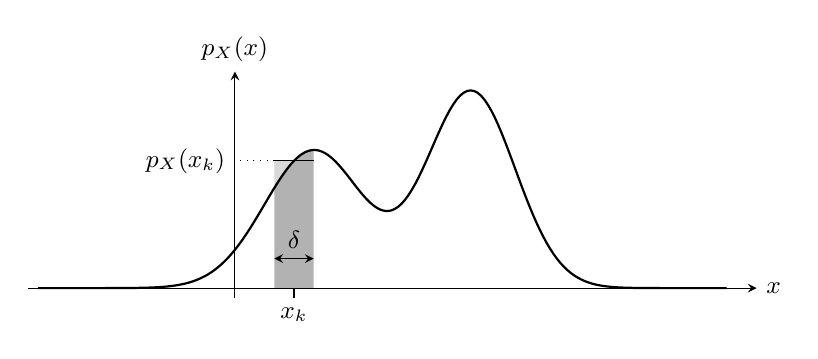
\begin{tikzpicture}
\shorthandoff{>}
%
% Cuantificacion de X
\begin{scope}[xscale=2.5,yscale=2.5]
%
\pgfmathsetmacro{\c}{.4};
\pgfmathsetmacro{\d}{1.2};
\pgfmathsetmacro{\s}{8};
\pgfmathsetmacro{\t}{10};
\pgfmathsetmacro{\a}{.7};
\pgfmathsetmacro{\b}{1};
%
\pgfmathsetmacro{\xk}{.3};
\pgfmathsetmacro{\dx}{.2};
%
\draw[>=stealth,->] (-1.05,0)--(2.65,0) node[right]{\small $x$};
\draw[>=stealth,->] (0,-.05)--(0,1.1) node[above]{\small $p_X(x)$};
%
% lei de proba
\draw[thick,domain=-1:2.5,samples=200] plot (\x,{(\a*exp(-\s*(\x-\c)^2)+\b*exp(-\t*(\x-\d)^2))});
%
% dominio alrededor de xk
\fill[domain=\xk-\dx/2:\xk+\dx/2,samples=20,opacity=.3]
({\xk-\dx/2},0)--
plot (\x,{(\a*exp(-\s*(\x-\c)^2)+\b*exp(-\t*(\x-\d)^2))})--
({\xk+\dx/2},0);
%
% xk y delta
\draw (\xk,0)--(\xk,-.05) node[below]{\small $x_k$};
\draw[>=stealth,<->] ({\xk-\dx/2},.15)--({\xk+\dx/2},.15);
\draw (\xk,.15) node[above]{\small $\delta$};
%
% recta sobre delta a altura de p(xk)
\draw ({\xk+\dx/2},{(\a*exp(-\s*(\xk-\c)^2)+\b*exp(-\t*(\xk-\d)^2))})--
({\xk-\dx/2},{(\a*exp(-\s*(\xk-\c)^2)+\b*exp(-\t*(\xk-\d)^2))});
\draw[dotted] ({\xk-\dx/2},{(\a*exp(-\s*(\xk-\c)^2)+\b*exp(-\t*(\xk-\d)^2))})--
(0,{(\a*exp(-\s*(\xk-\c)^2)+\b*exp(-\t*(\xk-\d)^2))}) node[left]{\small $p_X(x_k)$};
%
% dominio equivalente alrededo de xk
\fill[domain=\xk-\dx/2:\xk,samples=20,opacity=.15]
plot (\x,{(\a*exp(-\s*(\x-\c)^2)+\b*exp(-\t*(\x-\d)^2))})--
({\xk-\dx/2},{(\a*exp(-\s*(\xk-\c)^2)+\b*exp(-\t*(\xk-\d)^2))});
\end{scope}
\end{tikzpicture} \end{center}
%
\leyenda{Densidad de probabilidad $p_X$ de $X$, construcci\'on del alfabeto $\X$
  donde  se  define   la  versi\'on  cuantificada  $X^\delta$  de   $X$  con  su
  distribuci\'on discreta de probabilidad $p_{X^\delta}$. La superficia en grise
  oscuro es igual a la superficia definida por el rectangulo en grise claro.}
%
\label{fig:SZ:CuantificacionX}
\end{figure}
%

Mas  all\'a  de  esta  notable  diferencia  entre  la  entropia  y  la  entropia
diferencial, la \'ultima depende de los estados,  es decir que si $Y = g(X)$ con
$g$  biyectiva,  no  se  conserva  la  entropia,  \ie  \underline{se  pierde  la
  propiedad~\ref{prop:SZ:biyeccion}}  del  caso discreto:
%
\begin{eqnarray*}
H(Y) & = & - \int_{\Rset^d} p_Y(y) \log p_Y(y) \, dy\\[2.5mm]
%
& = &  - \int_{\Rset^d} p_Y(g(x)) \log p_Y(g(x)) \, |\Jac_g(x)| \, dx\\[2.5mm]
%
& = & - \int_{\Rset^d} p_Y(g(x)) \Big( \log \big( p_Y(g(x)) \, |\Jac_g(x)| \big) -
\log |\nabla^t g(x)| \Big) \, |\Jac_g(x)| \, dx
\end{eqnarray*}
%
donde $\Jac_g$ es la  matriz de componentes $\frac{\partial g_i}{\partial x_j}$,
Jacobiano  de  la  transformaci\'on  \   $g:  \Rset^d  \mapsto  \Rset^d$  \  ($g
\equiv  \begin{bmatrix} g_1(x_1  ,  \ldots  , x_d)  &  \cdots &  g_d(x_1  , \ldots  ,
  x_d)  \end{bmatrix}^t$) \  y  \  $|\cdot|$ representa  el  valor absoluto  del
determinente   de  la  matriz.    Recordandose  de   que  $p_X(x)   =  p_Y(g(x))
|\Jac_g(x)|$, se obtiene
%
\begin{propiedadesC}\setcounter{enumi}{\value{PropBiyeccion}}
%
\item\label{prop:SZ:biyeccionC}
Para  cualquier biyecci\'on $g:  \Rset^d \mapsto  \Rset^d$
  %
  \[
  H(g(X)) = H(X) + \int_{\Rset^d} p_X(x) \log |\Jac_g(x)| \, dx
  \]
  %
  donde el \'ultimo termino, $\Esp\left[  \log |\Jac_g(X)| \right]$ no vale cero
  en    general.   En    particular,   si    $H$   es    invariante    bajo   un
  deplazamiento,
  %
  \[
  H(X+\mu) = H(X) \quad \forall \: \mu \in \Rset^d
  \]
  %
  no  es invariante  por cambio  de escala,
  %
  \[
  H(a X) = H(X) + \log |a| \quad \forall \: a \in \Rset^*
  \]
\end{propiedadesC}
%
Esta  \'ultima relaci\'on  queda valid  para  $a$ matriz  invertible.  Por  esta
\'ultima  relaci\'on, se puede  ver que,  dado $X$,  cuando $a$  tiende a  0, la
entropia de  $a X$ tiende a  $-\infty$.  Es decir que,  para $a$ suficientemente
peque\~no,  se  puede  tener $H(a  X)  <  0$,  as\'i que  \underline{se  pierde}
tambi\'en \underline{la positividad, propiedad~\ref{prop:SZ:positividad}}.  Esta
perdida definitivamente quita la interpretaci\'on de incerteza/informaci\'on que
hubiera podido tener la entropia diferencial.  A veces, se usa lo que es llamado
potencia entropica:
%
\begin{definicion}[Potencia entropica]
  Sea $X$ una  variable aleatoria $d$-dimensional. La potencia  entropica de $X$
  es definida por
  %
  \[
  N(X) = \frac{1}{2 \pi \e} \exp\left( \frac2d H(X) \right)
  \]
\end{definicion}
%
\noindent Por construcci\'on,  $N(X) \ge 0$.  Ademas, en  el caso continuo, $N(a
X+b) = |a|^2 N(X)$ (queda valida para una matriz $a$ invertible): esta propiedad
puede justificar la idea de  ``potencia''; ademas $N(a X+b)$ tiende naturalmente
a cero cuando $a$ tiende a  cero.  Se recupera as\'i la noci\'on informacional a
trav\'es  de  $N$ en  este  contexto  ($a X  +  b$  ``tiende''  a $b$,  variable
deterministica).

Si se pierde  la propiedad de invarianza bajo  una biyecci\'on, sopredentemente,
se conserva la entropia bajo el equivalente continuo del rearreglo.
%
\begin{definicion}[Rearreglo simetrico]
  Sea $\P \subset \Rset^d$ abierto de  volumen finito $|\P| < +\infty$.  El {\it
    rearreglo simetrico}  $\P^\downarrow$ de  $\P$ es la  bola centrada en  0 de
  mismo volumen  que $\P$, \ie
  %
  \[
  \P^\downarrow  = \left\{  x  \in  \Rset^d \,  :  \: \frac{2  \pi^{\frac{d}{2}}
      |x|^d}{\Gamma\left(\frac{d}{2}\right)} \le |\P| \right\}
  \]
  %
  donde   $|\cdot|$   denota   la    norma   euclideana.    Eso   es   ilustrado
  figure~\ref{fig:SZ:ensemblerearreglado}-a.\newline  Sea $p_X$ una  densidad de
  probabilidad y sea $\P_t = \{ y \, : \: p_X(y) > t \}$ para cualquier $t > 0$,
  sus conjuntos  de niveles.  La densidad de  probabilidad~\footnote{Se proba de
    que  esta funci\'on,  positiva  por  definici\'on, suma  a  1.  Ademas,  por
    construcci\'on,  depende   unicamente  de   $|x|$  y  decrece   con  $|x|$.}
  rearreglada simetrica $p^\downarrow_X$ de $p_X$ es definida por
  %
  \[
  p^\downarrow_X(x)  =  \int_0^{+\infty}  \un_{\P_u^\downarrow}(x) \,  du
  \]
  %
  con $\un_A$ el indicator  del conjunto $A$, \ie $\un_A(x) = 1$  si $x \in A$ y
  cero sino.
\end{definicion}
%
Del hecho  de que $\forall \, t  < \tau \: \Leftrightarrow  \: \P_\tau \subseteq
\P_t  \:  \Leftrightarrow \:  \P_\tau^\downarrow  \subseteq \P_t^\downarrow$  es
sencillo   ver   que   si   $x   \in  \P_\tau^\downarrow$,   entonces   $x   \in
\P_t^\downarrow$, lo que conduce a  $p_X^\downarrow(x) > \tau$ y vice-versa. Mas
alla,  sobre $\P_{\tau+d\tau}  \backslash \P_\tau$  la funci\'on  $p_X$ ``vale''
$\tau$ \ y \ sobre $\P_{\tau+d\tau}^\downarrow \backslash \P_\tau^\downarrow$ la
funci\'on $p_X^\downarrow$  ``vale'' tambien $\tau$, lo que  da \ $\displaystyle
\int_{\P_\tau^\downarrow} p_X^\downarrow(x) \, dx = \int_{\P_\tau} p_X(x) \, dx$
(ver~\cite{LieLos01,   WanMad04}   para    une   prueba   mas   rigorosa).    La
representaci\'on de  la definici\'on es conocida como  representaci\'on en capas
de   pastel    (layer   cake    en   ingles).   Eso    es   ilustrado    en   la
figura~\ref{fig:SZ:ensemblerearreglado}-b
  %
  \begin{figure}[h!]
  %
  \begin{center} 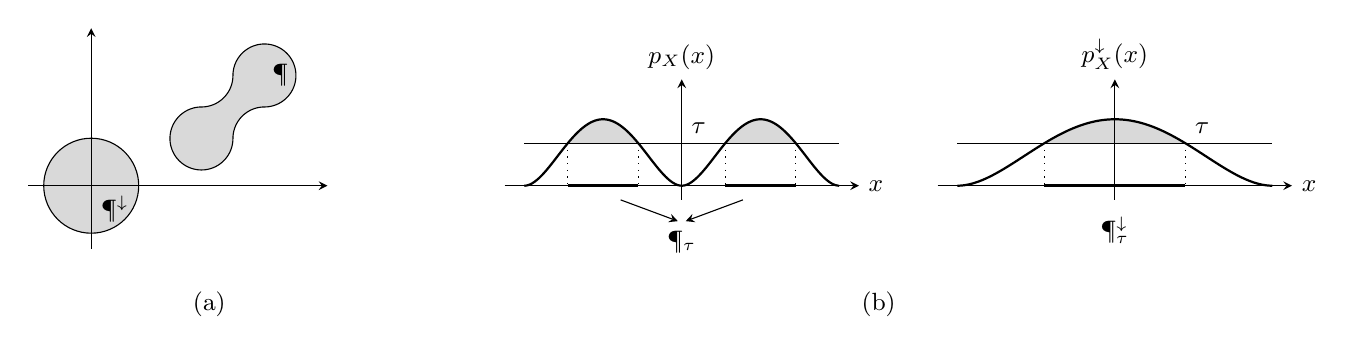
\begin{tikzpicture}
\shorthandoff{>}
%
\begin{scope}[scale=.4]
% Superficia 2*3 pi/4  + 2*2 - 2*pi/4 = 4+pi
\filldraw[draw=black,fill=gray!30]
   plot [domain=0:-270,samples=200] ({cos(\x)+3.5},{sin(\x)+1.5})
-- plot [domain=-90:0,samples=200] ({cos(\x)+3.5},{sin(\x)+3.5})
-- plot [domain=180:-90,samples=200] ({cos(\x)+5.5},{sin(\x)+3.5})
-- plot [domain=90:180,samples=200] ({cos(\x)+5.5},{sin(\x)+1.5})
-- cycle;
\draw (6,3.5) node {\small $\P$};
%
% superficia rearreglada
\filldraw[draw=black,fill=gray!30] (0,0) circle ({sqrt(1+4/pi)});
\draw (.75,-.75) node {\small $\P^\downarrow$};
%
% ejes
\draw[>=stealth,->] (-2,0)--(7.5,0);
\draw[>=stealth,->] (0,-2)--(0,5);
%
\end{scope}
%
%
%----------------------------------------
%
% p_X(x), P_tau...
\begin{scope}[xshift=7.5cm,yscale=1.8]
\pgfmathsetmacro{\t}{.3};
\pgfmathsetmacro{\xt}{sqrt(1-sqrt(32*\t/15))};
\pgfmathsetmacro{\dx}{5.5};% shift para p*(x)
\pgfmathdeclarefunction{studr}{1}{\pgfmathparse{(15/32)*((1-(#1)^2)^2)}}; %Student-r
%
% mezcla de Student-r 15/16 * (1-x^2)^2 (nu = 5) centrados en -1 y 1
% 15/32 (1-(x-a)^2)^2 > t iif (x-a)^2 < 1-sqrt(32*t/15)
% i.e. a-sqrt(1-sqrt(32*t/15)) < x < a+sqrt(1-sqrt(32*t/15))
\fill[domain=-1-\xt:-1+\xt,fill=gray!30] plot(\x,{studr(\x+1)}); % p(x) > tau, x < 0
\fill[domain=1-\xt:1+\xt,fill=gray!30] plot(\x,{studr(\x-1)}); % p(x) > tau, x > 0
\draw[thick,domain=-2:0,samples=100] plot(\x,{studr(\x+1)}); % p(x), x < 0
\draw[thick,domain=0:2,samples=100] plot(\x,{studr(\x-1)}); % p(x), x > 0
\draw (-2,\t)--(2,\t); \draw (0,\t) node[above right]{\small $\tau$}; % y = tau
%
% dominio P_tau
\draw[dotted] ({-1-\xt},{studr(\xt)})--({-1-\xt},0);
\draw[dotted] ({-1+\xt},{studr(\xt)})--({-1+\xt},0);
\draw[very thick] ({-1-\xt},0)--({-1+\xt},0);
\draw[>=stealth,->] ({-1+\xt/2},-.1)--(-.05,-.25);
%
\draw[dotted] ({1-\xt},{studr(\xt)})--({1-\xt},0);
\draw[dotted] ({1+\xt},{studr(\xt)})--({1+\xt},0);
\draw[very thick] ({1-\xt},0)--({1+\xt},0);
\draw[>=stealth,->] ({1-\xt/2},-.1)--(.05,-.25);
%
\draw (0,-.25) node[below]{\small $\P_\tau$};
%
% ejes
\draw[>=stealth,->] (-2.25,0)--(2.25,0) node[right]{\small $x$};
\draw[>=stealth,->] (0,-.1)--(0,.75) node[above]{\small $p_X(x)$};
%
%---------------------------
%
% 15/32 (1-(x-a)^2)^2 > t iif (x-a)^2 < 1-sqrt(32*t/15)
% i.e. a-sqrt(1-sqrt(32*t/15)) < x < a+sqrt(1-sqrt(32*t/15))
% Volumen 2*sqrt(1-sqrt(32*t/15))
% Por simetria, P_t* = [-2*sqrt(1-sqrt(32*t/15)) , 2*sqrt(1-sqrt(32*t/15))]
% da f*(x) = 15/32 (1-x^2/4)^2
\fill[domain=-2*\xt:2*\xt,fill=gray!30] plot({\x+\dx},{studr(.5*\x)}); % p*(x) > tau
\draw[thick,domain=-2:2,samples=200] plot({\x+\dx},{studr(.5*\x)});
\draw ({-2+\dx},\t)--({2+\dx},\t); \draw ({2*\xt+\dx},\t) node[above right]{\small $\tau$}; % y = tau
%
% dominio P_tau*
\draw[dotted] ({-2*\xt+\dx},{studr(\xt)})--({-2*\xt+\dx},0);
\draw[dotted] ({2*\xt+\dx},{studr(\xt)})--({2*\xt+\dx},0);
\draw[very thick] ({-2*\xt+\dx},0)--({2*\xt+\dx},0);
%
\draw (\dx,-.15) node[below]{\small $\P_\tau^\downarrow$};
%
% ejes
\draw[>=stealth,->] ({-2.25+\dx},0)--({2.25+\dx},0) node[right]{\small $x$};
\draw[>=stealth,->] (\dx,-.1)--(\dx,.75) node[above]{\small $p_X^\downarrow(x)$};
\end{scope}
%
\draw (1.5,-1.5) node{\small (a)};
\draw (10,-1.5) node{\small (b)};
\end{tikzpicture} \end{center}
  %
  \leyenda{(a):  Ilustraci\'on  del rearreglo  simetrico  $\P^\downarrow$ de  un
    conjunto  $\P$,  siendo  la  bola  centrada  en 0  de  mismo  volumen.   (b)
    Construcci\'on  del rearreglo  $p_X^\downarrow$:  dado un  $\tau$, se  busca
    $\P_\tau$ y  se deduce $P_\tau^\downarrow$; dado  un $x$, se  busca el mayor
    $t$  tal  que  $x  \in  P_t^\downarrow$, este  $t$  maximo  siendo  entonces
    $p_X^\downarrow(x)$;  ademas, por construcci\'on,  las superficias  en grise
    son iguales.}
  %
  \label{fig:SZ:ensemblerearreglado}
  \end{figure}
% =  \B  \left( 0  , r_\P  \right)$ con  $\frac{2
%    \pi^{d/2} r_\P^d}{\Gamma(d/2)} = |\P|$.

\begin{propiedadesC}\setcounter{enumi}{\value{PropPermutacion}}
\item\label{prop:SZ:permutacionC} {\it invarianza  bajo un rearreglo:} Sea $p_X$
  densidad   de  probabilidad   sobre   un  abierto   de  $\Rset^d$,
  %
  \[
  H\left( p_X^\downarrow \right) = H(p_X)
  \]
\end{propiedadesC}
%
\noindent Esta  propiedad es probada para  funciones convexas de  la densidad de
probabilidad              por             ejemplo             en~\cite{LieLos01}
o~\cite[Lema~7.2]{WanMad04}~\footnote{En~\cite[Sec.~3.3]{LieLos01}  lo  muestran
  para $\phi(p_X)$  donde $\phi$  es la diferencia  de dos  funciones monotonas,
  siendo $\phi(t)  = t  \log t$ un  caso particular.},  y entonces para  el caso
particular $\phi(t) = t \log t$.

Una pregunta  natural es saber  que se pasa  en termino de mayorizaci\'on  en el
contexto  continuo $d$-dimensional. Por  eso, se  necesita primero  redefinir la
noci\'on de mayorizaci\'on en este contexto:
%
\begin{definicion}[Mayorizaci\'on en el contexto continuo]\label{def:SZ:MayorizacionC}
  Una densidad  de probabilidad $p$  es dicha mayorizada por  una distribuci\'on
  $q$:
  %
  \[
  p  \prec q  \quad \mbox{ssi}  \quad \int_{\B(0,r)}  p^\downarrow(x) \,  dx \le
  \int_{\B(0,r)} q^\downarrow(x)  \, dx  \quad \forall \,  r > 0  \quad \mbox{y}
  \quad \int_{\Rset^d} p^\downarrow(x) \, dx = \int_{\Rset^d} q^\downarrow(x) \,
  dx
  \]
  %
  donde $\B(0,r) = \{  x \in \Rset^d: \: \|x\| \ge r \}$  es la bola centrada en
  $0$ y de rayo $r$ (las \'ultimas integrales son obviamente igual a 1).
\end{definicion}
%
\noindent  La Schur-concavidad~\ref{prop:SZ:Schurconcavidad}  se conserva  en el
caso  continuo, \ie
%
\[
p \prec  q  \quad \Rightarrow  \quad H(p)  \ge H(q)
\]
%
La desigualdad inversa es probada  para cualquier funci\'on $\phi$ convexa de la
densidad~\cite{Cho74} o~\cite[Prop.~7.3]{WanMad04},  en particular para $\phi(t)
= t \log t$.

Como  se lo  ha visto,  la  entropia diferencial  no es  siempre positiva,  como
consecuencia  de~\ref{prop:SZ:biyeccionC}.   Tambi\'en,  la  propiedad  de  cota
superior,  \underline{propiedad~\ref{prop:SZ:cotamaxima} se pierde}  en general,
\underline{salvo si se pone vinculos}:
%
\begin{propiedadesC}\setcounter{enumi}{\value{PropCotamaxima}}
\item
  \begin{enumerate}
  \item\label{prop:SZ:cotamaximauniforme} Si $\X$ es de volumen finito $|\X| < +
    \infty$, la entropia es acotada por arriba,
    %
    \[
    H(X) \le \log |\X|
    \]
    %
    con igualdad ssi $X$ es \underline{uniforme}.
    %
  \item\label{prop:SZ:cotamaximagaussiana}  Si  $\X =\Rset^d$  y  $X$ tiene  una
    matriz  de covarianza  dada  $\Sigma_X  = \Esp\left[  X  X^t \right]$  donde
    $\cdot^t$  denota  la transpuesta,  la  entropia  es  tambi\'en acotada  por
    arriba,
    %
    \[
    H(X) \le \frac{d}{2} \log(2 \pi \e) + \frac12 \log |\Sigma_X|
    \]
    %
    con igualdad  ssi $X$ es \underline{gaussiana}.  En  particular, la potencia
    entropica de  la gaussiana vale $N(X) =  \left| \Sigma_X \right|^{\frac1d}$,
    dando de nuevo un  ``sabor'' de potencia a $N$.  Como se o  va a ver en este
    cap\'itulo,  la  gaussiana  juega  un   rol  central  en  la  teoria  de  la
    informaci\'on.
  \end{enumerate}
  En  ambos casos,  estas  desigualdades con  la  distribuci\'on maximizante  se
  obtienen resolviendo  el problema de  maximizaci\'on de la entropia  subjeto a
  vinculos.      Se     trata    del     caso     m\'as     general    en     la
  secci\'on~\ref{sec:SZ:MaxEnt}.
\end{propiedadesC}

Al      final,     \underline{se      conservan      las     propiedades      de
  concavidad~\ref{prop:SZ:concavidad},  de aditividad~\ref{prop:SZ:aditividad} y
  de sub-aditividad~\ref{prop:SZ:subaditividad}}.   Es interesante de  notar que
de  la desigualdad~\ref{prop:SZ:subaditividad},  puramente  entropica, se  puede
deducir la  desigualdad de Hadamard,  desigualdad puramente matricial:  $|R| \le
\prod_i  R_{i,i}$  para  cualquier  matriz simetrica  definida  positiva  (viene
de~\ref{prop:SZ:subaditividad} escrita  para una  gaussiana de covarianza  $R$ y
tomando una exponencial de la desigualdad).

% ================================== Mutua =================================== %

\seccion{Entropia condicional, informaci\'on mutua, entropia relativa}
\label{s:SZ:Mutua}

Tratando de un par de variable  aleatorias $X$ e $Y$, una cuesti\'on natural que
occure es de cuantificar la incerteza que queda sobre una de las variable cuando
se  observa  la  otra.  Dicho  de  otra  manera, si  se  mide  $Y  =  y$,  ?`que
informaci\'on lleva sobre  $X$? La respuesta a esta  interogaci\'on se encuentra
en la  noci\'on de entropia condicional. Si  uno mide $Y =  y$, la descripci\'on
estadistica de $X$ conociendo este $Y$ se resuma a la distribuci\'on condicional
de  probabilidad $p_{X|Y}  = \frac{p_{X,Y}}{p_Y}$.   Con esta  restricci\'on, se
puede  evaluar una  incerteza sobre  $X$, sabiendo  de que  $Y=y$,
%
\[
H(X|Y=y) = H\left( p_{X|Y}(\cdot,y) \right)
\]
%
Entonces, condicionalmente a la variable aleatoria $Y$, la incerteza va a ser el
promedio  estadistico sobre  todos los  estados $Y$  es decir  $H(X|Y)  = \sum_y
p_Y(y) H(X|Y=y)$:
%
\begin{definicion}[Entropia condicional]\label{def:SZ:entropiacondicional}
  Sean $X$ e $Y$ dos  variables aleatorias discretas, la entropia condicional de
  $X$ sabiendo  $Y$ es  definida por
  %
  \[
  H(X|Y) = - \sum_{x,y} p_{X,Y}(x,y) \log p_{X|Y}(x,y)
  \]
\end{definicion}
%
Esta definici\'on se transpone naturalmente a la entropia diferencial:
%
\begin{definicion}[Entropia diferencial condicional]\label{def:SZ:entropiadiferencialcondicional}
  Sean $X$ e $Y$ dos  variables aleatorias continuas, la entropia condicional de
  $X$ sabiendo $Y$ es definida por
  %
  \[
  H(X|Y) = - \int_{\Rset^d} p_{X,Y}(x,y) \log p_{X|Y}(x,y) \, dx \, dy
  \]
\end{definicion}

Si $X$ e $Y$ son indepedientes, $p_{X|Y}$ se reduce a $p_X$, as\'i que vale cero
la entropia condicional:
%
\begin{propiedades}
\item\label{prop:SZ:independenciacondicional}
  %
  \[
  X \: \mbox{e} \: Y \: \mbox{independientes} \quad \Leftrightarrow \quad H(X|Y)
  = H(X)
  \]
\end{propiedades}
%
Esta  propiedad  vale  en ambos  casos,  discreto  como  continuo.  En  el  caso
discreto, se interpreta como el hecho  de que $Y$ no lleva ninguna informaci\'on
sobre $X$, y intonces ninguna medici\'on  de $Y$ va a cambiar la incerteza sobre
$X$.

Siendo $H(X|Y=y)$  una entropia,  va a  heredir de todas  las propiedades  de la
entropia  (diferencial).  Ademas,  de  $p_{X,Y}  = p_{X|Y}  p_Y$  de  deduce  la
propiedad siguiente (valida para la entropia como su extensi\'on diferencial)
%
\begin{propiedades}
\item\label{prop:SZ:cadena}  {\it Regla de  cadena}
  %
  \[
  H(X,Y) =  H(X|Y) +  H(Y)
  \]
  %
  Esta  regla, valida  en ambos  casos,  discreto como  continuo, se  generaliza
  sencillamente a
  %
  \[
  H(X_1 , \ldots , X_n) = H(X_1) + \sum_{i=2}^n H(X_i|X_{i-1} , \ldots , X_1)
  \]
  %
  De       esta       regla      de       cadena       se      recupera       la
  propiedad~\ref{prop:SZ:independenciacondicional}     a     partir    de     la
  propiedad~\ref{prop:SZ:aditividad}.
\end{propiedades}
%
Siendo  $H(X|Y=y)$  una   entropia,  en  el  caso  discreto   esta  cantidad  es
positiva. Entonces, en  el caso discreto, $H(X|Y)$ es positiva,  lo que proba la
la super-aditividad~\ref{prop:SZ:superaditividad}.

De la regla de  cadena $H(X,Y) = H(X|Y) + H(Y) = H(Y|X)  + H(X)$ aparece que las
cantidades  $H(X|Y)-H(X)$, $H(Y|X)-H(Y)$  y $H(X,Y)  -  H(X) -  H(Y)$ son  todas
iguales. Estas canditades definen lo que se llama la informaci\'on mutua entre \
$X$ \ e \ $Y$:

%
\begin{definicion}[Informaci\'on mutua]\label{def:SZ:mutua}
  Sean $X$ e $Y$ dos variables  aleatorias, la informaci\'on mutua entre \ $X$ \
  e  \ $Y$ \  es la  cantida simetrica
  %
  \[
  I(X;Y) = H(X|Y)-H(X) = H(Y|X)-H(Y) = H(X,Y) - H(X) - H(Y)
  \]
  %
  En el caso discreto se  expresa
  %
  \[
  I(X;Y)  =  \sum_{x,y}   p_{X,Y}(x,y)  \log  \left(  \frac{p_{X,Y}(x,y)}{p_X(x)
      p_Y(y)} \right)
  \]
  %
  y su forma diferencial, se escribe
  %
  \[
  I(X;Y)  = \int_{\Rset^d}  p_{X,Y}(x,y) \log  \left( \frac{p_{X,Y}(x,y)}{p_X(x)
      p_Y(y)} \right) \, dx \, dy
  \]
\end{definicion}

Las diferentes cantitades  peden ser vista a trav\'es  una visi\'on ensemblista,
como  descrita el la  figura~\ref{fig:SZ:Venn}. Este  diagrama es  conocido como
diagrama de Venn.
%
\begin{figure}[h!]
%
\begin{center} 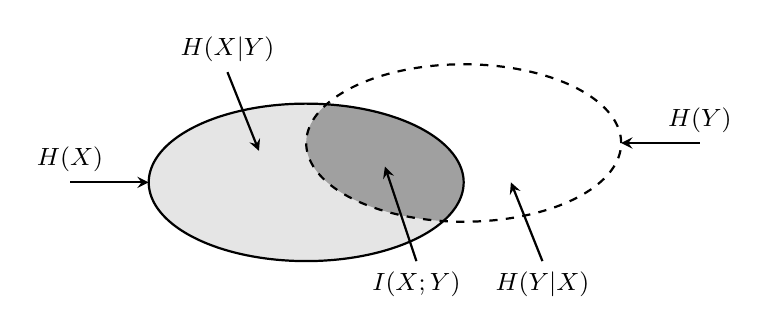
\begin{tikzpicture}[scale=2]
\shorthandoff{>}
% interior H(X) x^2 + 4 y^2 = 1 => y = \pm sqrt(1-x^2)/2
\fill[domain=0:360,samples=200,opacity=.1] plot ({cos(\x)},{.5*sin(\x)});
%
% interior H(Y) (x-1)^2 + 4 (y-1/4)^2 = 1 => y = 1/4 \pm sqrt(1-(x-1)^2)/2
% se cruzan cuando x = 1 \pm sqrt(55)/10 =>
% theta = acos(.5 \pm sqrt(55)/20) para X
% theta = acos(-.5 \pm sqrt(55)/20) para X
\pgfmathsetmacro{\s}{acos(.5-sqrt(55)/20)};
\pgfmathsetmacro{\t}{-acos(.5+sqrt(55)/20)};
\pgfmathsetmacro{\u}{-acos(-.5+sqrt(55)/20)};
\pgfmathsetmacro{\v}{acos(-.5-sqrt(55)/20)-360};
%
% interior I(X;Y)
%\draw[domain=\v:\v] plot ({cos(\x)+1},{.5*sin(\x)+.25}) node{$\bullet$};
\fill[opacity=.3]
   plot [domain=\s:\t,samples=200] ({cos(\x)},{.5*sin(\x)})
-- plot [domain=\u:\v,samples=200] ({cos(\x)+1},{.5*sin(\x)+.25})
-- cycle;
%
% borders H(X) y H(Y)
\draw[domain=0:360,samples=200,thick] plot ({cos(\x)},{.5*sin(\x)});
\draw[dashed,domain=0:360,samples=200,thick] plot ({cos(\x)+1},{.5*sin(\x)+.25});
%
% flechas y flechas condicionales
\draw[thick,>=stealth,<-] (-1,0)--(-1.5,0) node[above]{\small $H(X)$};
\draw[thick,>=stealth,<-] (-.3,.2)--(-.5,.7) node[above]{\small $H(X|Y)$};
%
\draw[thick,>=stealth,<-] (2,.25)--(2.5,.25) node[above]{\small $H(Y)$};
\draw[thick,>=stealth,<-] (1.3,0)--(1.5,-.5) node[below]{\small $H(Y|X)$};
%
\draw[thick,>=stealth,<-] (.5,.1)--(.7,-.5) node[below]{\small $I(X;Y)$};
\end{tikzpicture} \end{center}
%
\leyenda{Diagrama  de Venn:  Ilustraci\'on  de la  definici\'on  de la  entropia
  condicional,  informaci\'on  mutua, y  los  vinculos  entre  cada medida.   La
  superficia  del elipse en  linea llena  (parte grise)  representa $H(X)$  y el
  interior  de la en  linea punteada  representa $H(Y)$.   La parte  grise clara
  representa $H(X|Y)$  superficia del ``conjunto $H(X)$'' quitando  la parte que
  partenece  a  $H(Y)$.  La  parte  blanca  representa  $H(Y|X)$ superficia  del
  ``conjunto $H(Y)$''  quitando la  parte que partenece  a $H(X)$.  La  parte en
  grise oscuro es entonces lo que $X$ e $Y$ comparten, es decir $I(X;Y)$.}
%
\label{fig:SZ:Venn}
\end{figure}

Como se lo va a probar, $I$ es positiva; representa realmente una informaci\'on,
la compartida  entre \ $X$  \ e  \ $Y$. Si  de la incerteza  de $X$ se  quita la
incerteza  de  $X$   una  vez  que  $Y$  es  medida,  lo   que  queda  tiene  la
significaci\'on de la informaci\'on que  estas variables tienen en com\'un. Para
probar la positividad de $I$, se  introduce de manera mas general la noci\'on de
entropia     relativa,     conocida     tambi\'en    como     divergencia     de
Kullback-Leibler~\cite{KulLei51, Kul68, CovTho06, Rio07}:
%
%\SZ{Buscar ref de Kullback and so on Kul68, }
%
\begin{definicion}[Entropia relativa]\label{def:SZ:entropiarelativa}
  La entropia relativa, o divergencia de una distribuci\'on de probabilidad $q$,
  con  respeco  a una  distribuci\'on  de  referencia  $p$, donde  \underline{el
    alfabeto   de   definici\'on   de    $p$   (o   soporte)   incluye   lo   de
    $q$}, es definida como
  %
  \[
  \Dkl[q]{p} = \sum_x q(x) \log \left( \frac{q(x)}{p(x)} \right)
  \]
  %
 o, en su forma diferencial
  %
 \[
 \Dkl[q]{p} = \int_{\Rset^d} q(x) \log \left( \frac{q(x)}{p(x)} \right) \, dx
 \]
  %
 (en este \'ultimo caso, la condici\'on de inclusi\'on del soporte de $q$ dentro
 del de $p$ se  formula como de que $q$ es absolutamebte  continua con respeto a
 $p$)~\footnote{M\'as rigorosamente, en el  caso discreto, esta cantidad depende
   solamente de $p$ y  $q$ y no de los estados. La  condici\'on necesaria es que
   $p$ y $q$  tienen los mismos n\'umeros de componentes  (se completa el vector
   lo mas corto) y  si la $i$-esima componente de $q$ vale  cero, entonces la de
   $p$ vale cero  tambi\'en.  Ademas, con $p$ y $q$ de  mismo tama\~no, se puede
   poner en  biyecci\'on los  alfabetos asociados  a $p$ y  $q$, sin  perdida de
   generalidad.  En el  caso continuo,  esta  razonamiento no  vale m\'as,  esta
   cantidad dependiendo de los estados\ldots}.
\end{definicion}
%
Inicialmente, esta  medida fue introducido por  Kullback y Leibler  con la misma
linea  que   Shannon,  interpretando  $\log\left(\frac{q}{p}\right)$   como  una
informaci\'on de  discriminaci\'on entre dos  hypotesis de distribuciones  $q$ y
$p$  por  la  obsrvaci\'on  $x$,  la  divergencia  siendo  la  informaci\'on  de
discriminaci\'on promedia.  Introdujeron tambi\'en una  versi\'on simetriza, que
veremos mas adelante.

Esta medida  puede ser  vista tambi\'en como  una entropia de  la distribuci\'on
$q$, relativamente  a una distribuci\'on de  referencia $p$. Por  ejemplo, en el
caso discreto finito, si $p$ es  la distribuci\'on uniforme sobre un alfabeto de
cardinal  $\alpha$, $\Dkl[q]{p} =  \log \alpha  - H(q)$,  lo que  representa una
desviaci\'on  de la  entropia con  su valor  maximal. La  misma interpretaci\'on
queda en  el caso continuo  con la  lei uniforme ($p$  y $q$ definidas  sobre el
mismo espacio de  volumen finito) o con  la gaussiana ($p$ y $q$  dando la misma
matriz de  covarianza). {\it  Como para la  entropia, cuando se  necesitar\'a un
  logaritmo   especificamente  de   base   $a$,  se   notar\'a  la   divergencia
  $D_{\mathrm{kl},a}$.}

\begin{lema}[Positividad de la entropia relativa]
  %
  \[
  \Dkl[q]{p} \ge 0 \quad \mbox{con igualdad ssi} \quad p = q \: (c.s.)
  \]
  %
  donde $(c.s.)$ significa ``casi siempre''.
\end{lema}
%
\begin{proof}
  Existen varias pruebas,  pero la mas linda puede ser  la usando la desigualdad
  de   Jensen:   para   $\phi$   estrictamente   convexa,   $\Esp[\phi(X)]   \ge
  \phi(\Esp[X])$ con igualdad ssi $X$  es deterministica (casi siempre). Sea $X$
  de distribuci\'on  o densidad de probabilidad  $p$.  En el  caso discreto como
  diferencial,  se  escribe  la   entropia  relativa  $\Dkl[q]{p}  =  \Esp\left[
    \frac{q(X)}{p(X)} \log \left( \frac{q(X)}{p(X)}  \right) \right]$.  Sea $Y =
  \frac{q(X)}{p(X)}$   y  $\phi(u)   =  u   \log  u$,   funci\'on  estrictamente
  convexa. Entonces $\Dkl[q]{p} = \Esp[\phi(Y)] \ge \phi(\Esp[Y])$. Con $\Esp[Y]
  = \Esp\left[ \frac{q(X)}{p(X)} \right] = \sum_x  q(x) = 1$ (y con una integral
  en el  caso diferencial)  y $\phi(1)  = 0$ sz  termina la  prueba. El  caso de
  igualdad apareciendo  ssi $Y$ es deterministica,  es decir $\frac{p(X)}{q(X)}$
  deterministica, es equivalente a $p(x) \propto  q(x) \: (c.s.)$, \ie $p = q \:
  (c.s.)$ porque ambas suman a uno.
\end{proof}


\SZ{Eso es la desigualdad de Gibbs}

Esta propiedad, valide  en el caso discreto como  continuo, tiene consecuencias,
cuando  se fije  de que
%
\[
I(X;Y) = \Dkl[p_{X,Y}]{p_X p_Y}
\]
%
\ie  la  informaci\'on  mutua  es  la  divergencia  de  Kullback-Leibler  de  la
distribuci\'on conjunta relativa al producto de las marginales.
%
\begin{propiedades}
\item\label{prop:SZ:Ipositive}   {\it   $I$   es   positiva,  como   medida   de
    independencia:}
  %
  \[
  I(X;Y) \ge 0 \quad \mbox{con igualdad ssi $X$ e $Y$ son independientes}
  \]
%
\item\label{prop:SZ:condicionar} {\it  Condicionar reduce la  entropia}
  %
  \[
  H(X|Y) \le H(X) \quad \mbox{con igualdad ssi $X$ e $Y$ son independientes}
  \]
  %
  Esta    desigualdad,     con    la     regla    de    cadena,     prueba    la
  sub-aditividad~\ref{prop:SZ:subaditividad}.    Esta    reducci\'on   vale   en
  promedio, pero el conocimiento de un valor particular puede ser tal que $H(X|Y
  = y) > H(X)$, \ie aumentar la entropia!  (ver ejemplos en~\cite[p.~59]{Rio07})
\end{propiedades}

Fijense   que  si   $\Dkl{}$  es   positiva,  \underline{no   es   simetrica}  y
\underline{tampoco no satisface  la desigualdad triangular}. Por eso,  no es una
distancia  y  tiene  el  nombre  de {\it  divergencia}.   La  distribuci\'on  de
referencia $p$ juega un rol fundamental.

Al  final, a  pesar  de que  la forma  diferencial  de $\Dkl{}$  depende de  los
estados, queda invariante bajo  una misma transformaci\'on biyectiva sobre ambos
$p$ y $q$.


% ================================== Fisher ================================== %

\seccion{Informaci\'on de Fisher}
\label{Ssec:SZ:Fisher}

Si la  entrop\'ia y las heramientas  relacionadas son naturales como  medidas de
informaci\'on, no se  puede resumir una distribuci\'on a una  medida escalar. En
el marco  de la teor\'ia  de la  estimaci\'on, R. Fisher~\footnote{De  hecho, la
informaci\'on de  Fisher habia  estudiado antes  por varios  estatisticianos tal
como  F.  Y.  Edgeworth  en 1908-1909  o  a\'un  antes, en  1898  por Pearson  y
Fillon~\cite{Hal06, Edg08,  PeaFil98}. Adem\'as,  le versi\'on  multivariada fue
introducida m\'as tarde, por Doob~\cite{Doo34, Doo36}} introdujo una noci\'on de
informaci\'on intimamente  relacionada al error cuadr\'atico  en la estimaci\'on
de   un  par\'ametro   a  partir   de  una   variable  parametrizado   por  este
par\'ametro~\cite{Fis22, Fis25:07, Kay93, LehCas08, Bos07, CovTho06, Fri04}.

\modif{
\begin{definicion}[Matriz informaci\'on de Fisher param\'etrica con respecto a una medida]
\label{Def:SZ:MatrizFisherParametricaMu}
%
  Sea   $X$   una   variable   aleatoria  parametrizada   por   un   par\'ametro
  $m$-dimensional,   $\theta  \in   \Theta  \subset   \Rset^m$,  de   medida  de
  probabilidad  $P_X(\cdot ;  \theta)$ que  admite una  densidad de  probabilidad
  $p_X(\cdot;\theta)$  con respecto  a  una medida  $\mu$  dada, definida  sobre
  $\X  \subset \Rset^d$  su soporte.   Suponga que  $p_X$ sea  diferenciable con
  respecto  a  $\theta$  sobre  $\Theta$.   La matriz  de  Fisher,  de  tama\~no
  $m \times m$, es definida por
  %
  \begin{eqnarray*}
    J_\theta(X    \|    \mu)  &  = &    \Esp\left[    \Big(    \nabla_\theta    \log
    p_X(X;\theta) \Big)  \Big( \nabla_\theta \log p_X(X;\theta)  \Big)^t \right]\\[2.5mm]
    %
    & = & \int_\X \, \left( \nabla_\theta \log \left( \frac{dP_X}{d\mu}(x;\theta) \right)
    \right) \left( \nabla_\theta \log \left( \frac{dP_X}{d\mu}(x;\theta) \right)
    \right)^t \, dP_X(x;\theta)
  \end{eqnarray*}
  %
  donde \  $\nabla_\theta = \left[ \cdots  \: \frac{\partial}{\partial \theta_i}
    \: \cdots  \right]^t$ \  es el gradiente  en \  $\theta$ \ y  \ $\log$  \ el
  logaritmo natural.  Es la matriz de covarianza del {\it score param\'etrico} \
  $S_\theta(X) =  \nabla_\theta \log  p_X(X;\theta)$ \ notando  que su  media es
  igual a cero (escribiando el  promedio y intercambiando integral y gradiente),
  siendo  \  $\log p_X$  \  la  {\it  log-verosimilitud}.  Bajo  condiciones  de
  regularidad, se puede mostrar~\footnote{Es  una consecuencia del teorema de la
    divergencia, suponiendo que los bordes del soporte \ $\X$ \ no dependen de \
    $\theta$ \  y que  la funci\'on score  se cancela  en estos bordes.}   que
    %
    \[
    J_\theta(X  \|  \mu) =  -  \Esp\big[  \Hess_\theta  \log p_X(X;\theta)  \big]  =
    - \int_\X \, \Hess_\theta \left( \log \left( \frac{dP_X}{d\mu}(x;\theta) \right) \right)\,
    dP_X(x;\theta)
    \]
    %
    \ con $\Hess_\theta$  la  Hessiana
  %~\footnote{Recordamos de que,  para \  $f: \Rset^m  \mapsto \Rset,
  %  \quad  \Hess_\theta f$  \ es  la matriz  de componentes  \ $\frac{\partial^2
  %    f}{\partial \theta_i  \partial \theta_j}$.}
  %\ de  \ $\log  p_X(X;\theta)$
  (ver notaciones).  Nota: a veces se define la informaci\'on de Fisher como
  %
  \[
  \Tr(J_\theta(X \| \mu ))    =     \Esp\left[    \Big\|     \nabla_\theta    \log
  p_X(X;\theta)   \Big\|^2   \right]   =   -   \Esp\big[   \Delta_\theta   \log
  p_X(X;\theta) \big] \]
  %  
  traza~\footnote{Recordar que para dos vectores $a$ y  $b$, $\Tr a b^t = b^t a$
  y que  $\Tr \Hess  = \div  \nabla =  \Delta$ (ver  notaciones).} de  la matriz
  informaci\'on de Fisher.
\end{definicion}
%
Como  para  la  entrop\'ia,  la  matriz  de Fisher  se  escribe  generalmente  \
\modif{$J_\theta(X \| \mu)$, \ a pesar de que no sea  funci\'on de \ $X$ \ pero de la densidad
de  probabilidad y de la medida $\mu$}.  Se  la  notar\'a  tambi\'en
%
\[
\modif{J_\theta(p_X \| \mu) \equiv J_\theta(P_X \| \mu) \equiv J_\theta(X \| \mu)}
\]
%
seg\'un la escritura la m\'as conveniente.
}

Notar  que para  une  distribuci\'on  de la  familia  exponencial natural  vista
secci\'on~\ref{Ssec:MP:FamiliaExponencial},   \modif{de  densidad   $p_X(x;\eta)
= \exp\left( \eta^t S(x) - \varphi(\eta) \right)$  \ con respecto a una medida \
$\mu$,}  \  tenemos   \  $S_\eta(x)  =  \nabla_\eta  \log   p_X(x;\eta)  =  S(x)
- \nabla \varphi(\eta) = S(x) - \Esp[S(X)]$ as\'i que
%
\[
\modif{J_\eta(X \| \mu) = \Cov[S(X)] = \Hess_\eta \varphi(\eta)}
\]
%
(ver por ejemplo~\cite{LehCas98, Bos07}).
% resp p. 116, p. 33

\modif{Cuando la densidad de proablidad es continua y
%En el caso  continuo, $\mu = \mu_L$, con una  densidad
diferenciable, tomando el
gradiente en \ $x$  \ en lugar de \ $\theta$ \ da  la matriz de informaci\'on de
Fisher no param\'etrica,
%
\begin{definicion}[Matriz informaci\'on de Fisher no param\'etrica con respecto a una medida]
\label{Def:SZ:MatrizFisherNoParametricaMu}
%
  Sea \ $X$  \ una variable aleatoria  de medidad de probabilidad \  $P_X$ \ que
  admite una  densidad de  probabilidad \  $p_X$ \  con respecto  a una  medida \
  $\mu$ \  dada, definida sobre  \ $\X \subset  \Rset^d$ \ su  soporte.  Suponga
  que \ $p_X$ \ sea continua y diferenciable con respecto a \ $x$.  La matriz de
  Fisher no param\'etrica $d \times d$ es definida por
  %
  \begin{eqnarray*}
  J(X \| \mu) & = &  \Esp\left[ \Big(  \nabla_x \log p_X(X)  \Big) \Big(  \nabla_x \log
      p_X(X) \Big)^t \right]\\[2.5mm]
  %
  & = & \int_\X \, \left(  \nabla_x \log \left( \frac{dP_X}{d\mu}(x) \right)  \right)
  \left(  \nabla_x \log \left( \frac{dP_X}{d\mu}(x) \right)  \right)^t \, dP_X(x)
  \end{eqnarray*}
  %
  Es  la matriz  de covarianza  de  la {\it  funci\'on score}  \ $\nabla_x  \log
  p_X(X)$ \ (escribiendo la media y $p_X$  siendo cero el los bordes de $\X$, se
  ve que  el promedio  de $\nabla_x  \log p_X(X)$ tambi\'en  vale cero)  o, bajo
  condiciones de regularidad,
  %
  \[
  J(X \| \mu) = - \Esp[\Hess_x \log p_X(X)]
  = \int_\X \left( \Hess_x \log\left( \frac{dP_X}{d\mu}(x)\right) \right) \, dP_X(x)
  \]
  % menos el promedio de la Hessiana en \ $x$ \ de la log-verosimilitud.  
  Como para el caso param\'etrico, a  veces se define la informaci\'on de Fisher
  no-parametrica como
  %
  \[  
  \Tr(J(X \| \mu ))  =  \Esp\left[  \Big\|  \nabla_x  \log  p_X(X)  \Big\|^2  \right]  =
  - \Esp\big[ \Delta_x \log p_X(X) \big] \]
  % 
  traza de  la matriz  informaci\'on de Fisher.
\end{definicion}
}
%
\modif{Como para la entrop\'ia, y la matriz  de Fisher parametrica, la matriz de Fisher
no parametrica es funci\'on de distribuci\'on o densidad y $\mu$ y se la notar\'a tambi\'en
%
\[
J(p_X \| \mu) \equiv J( P_X \| \mu ) \equiv J(X \| \mu)
\]
}
%
seg\'un la escritura la m\'as conveniente.

\modif{
En la  literatura se  encuentra mayormente  el caso  donde $\mu  = \mu_L$  es la
medida de Lebesgue,  o cuando $\mu$ es  una medida de probabilidad, lo  que va a
dar respectivamente la informaci\'on de  Fisher (impl\'icito ``con respecto a la
medida de Lebesgue'') y la divergencia de Fisher~\cite[Def.~13]{Joh04} o~\cite{JohBar04}:
%
\begin{definicion}[Informaci\'on de Fisher y divergencia de Fisher o informaci\'on de Fisher relativa]
\label{Def:SZ:MatrizFisherDivergencia}
%
Sea     $X$      que     satisface      a     los     requisitos      de     las
definiciones~\ref{Def:SZ:MatrizFisherParametricaMu}
o~\ref{Def:SZ:MatrizFisherNoParametricaMu} seg\'un el caso. Entonces
%
\begin{itemize}
\item Cuando  $\mu =  \mu_L$  se  hablar\'e simplemente  de  {\it  matriz de  Fisher},
respectivamente param\'etrica y no param\'etrica)  y se notar\'a esta matriz sin
mencionar $\mu_L$,
%
\[
\mbox{Notaci\'on para } \: \mu = \mu_L \: \mbox{Lebesgues: } \: J_\theta(X) \equiv J_\theta(p_X) \quad \mbox{y} \quad J(X) \equiv J(p_X).
\]
%
\item Cuando $\mu  = Q$  es una  medida de probabilidad,  $J_\theta(P_X \|  Q)$ \  y \
$J(P_X \| Q)$  son llamadas {\it divergencia de Fisher}  o {\it informaci\'on de
Fisher relativa}, $Q$  jugando un rol de referencia (al  imagen de la entrop\'ia
relativa)~\cite{}.
%
\item Si  \ $P_X$  \ y  \ $Q$  \  admiten una  densidad con  respecto a  una medida $\mu$,  respectivamente  \   $p_X$  \  y  \  $q$,  se   escribe  tambi\'en
%
\[
J_\theta(p_X                                \|                                q)
= \int_\X \left( \nabla_\theta \log\left( \frac{p_X(x)}{q(x)} \right) \right)
\left( \nabla_\theta \log\left( \frac{p_X(x)}{q(x)} \right) \right)^t \, dQ(x)
\]
%
y
%
\[
J(p_X \| q) = \int_\X \left( \nabla_x \log\left( \frac{p_X(x)}{q(x)} \right) \right)
\left( \nabla_x \log\left( \frac{p_X(x)}{q(x)} \right) \right)^t \, dQ(x) 
\]
\end{itemize}
\end{definicion}

Si la matriz de Fisher depende de la medida de referencia en general, aparece que, en el caso parametrico, queda constante si se considera una otra referencia tal que la derivada de Rado-Nykodym de la primera con respecto a la secunda no depende del parametro:
%
\begin{lema}[Matriz de Fisher parametrica inariante por cambio de medida]
  Sea        $X$        variable       aleatoria        parametrizada        por
  $\theta  \in \Theta  \subset \Rset^m$,  de medida  de probabilidad  $P_X(\cdot
  ; \theta)$.  Sean  dos  medidas  \  $\mu,   \nu$  \  tales  que  \  $P_X(\cdot
  ; \theta) \ll  \mu \ll \nu$ \  y \ $\frac{d\mu}{d\nu}$ \  sea independiente de
  $\theta$. Supone que  la densidad \ $\frac{dP_X(\cdot ;  \theta)}{d\mu}$ \ sea
  diferenciable en \ $\theta$ \ sobre \ $\Theta$. Entonces  la densidad \ $\frac{dP_X(\cdot ;  \theta)}{d\mu}$ \ es
  diferenciable en \ $\theta$ \ sobre \ $\Theta$ \ y
  %
  \[
  J_\theta( X \| \nu) = J_\theta( X \| \mu )
  \]
  %
  En particular, la matriz de Fisher queda la misma para cualquier $\mu$ independiente del parametro.
\end{lema}
%
\begin{proof}
La   prueba   sigue  obviamente   del   lema~\ref{Lem:RelacionesDerivadasRadon},
$\frac{dP_X(\cdot        ;        \theta)}{d\nu}       =        \frac{dP_X(\cdot
; \theta)}{d\mu} \frac{d\mu}{d\nu}$: el secundo factor siendo independiente de \
$\theta$,   por   un   lado   la  diferenciabilidad   de   \   $\frac{dP_X(\cdot
; \theta)}{d\mu}$ \ implica la de \ $\frac{dP_X(\cdot ; \theta)}{d\nu}$ y por el
otro  lado  por  el  logaritmo  y  derivada en  \  $\theta$  \  el  t\'ermino  \
$\frac{d\mu}{d\nu}$  desaparece de  integrante en  la  formula de  la matriz  de
Fisher.
%(ver tambi\'en lema~\ref{Lem:RelacionIntegracionDerivadasRadon}).
\end{proof}
%
}

Es interesante notar que:
%
\begin{itemize}
\item Volviendo a una familia param\'etrica \ $p_X(\cdot;\theta)$, cuando \ $\theta$ \
es un  par\'ametro de posici\'on,  en el  caso de distribuci\'on  admitiendo una
densidad,  \ $p_X(x;\theta)  =  p(x  - \theta)$,  \  $\nabla_\theta  \log p_X  =
- \nabla_x \log  p_X$ \ tal  que la informaci\'on  param\'etrica se reduce  a la
informaci\'on no param\'etrica.
%
\item Si \ $X$ \ es gaussiano  de matriz de covarianza \ $\Sigma_X$, entonces se
  muestra sencillamente que \ $J(X) = \Sigma_X^{-1}$ \ matriz de precisi\'on (o,
  de  una  forma,  inversa  de  la dispersi\'on  o  incerteza  en  t\'ermino  de
  estad\'isticas de orden 2).
%
\item Es sencillo ver  que, por definici\'on \ \modif{$J_\theta(X \| \mu)$ \ y  \ $J(X \| \mu)$} \ son
  sim\'etricas y que \ \modif{$J_\theta(X \| \mu) \ge 0$ \ y \ $J(X \| \mu) \ge 0$ \ \ie $J_\theta(X \| \mu) \in
  \Pos_m(\Rset), \:\: J(X \| \mu) \in \Pos_m(\Rset)$}~\cite{LehCas98}.  Adem\'as,
  %
  \[
  \forall \ A \ \mbox{matrix no singular}, \quad \modif{J(AX \| \mu) = A^{-t} J(X \| \mu) A^{-1}},
  \]
  %
  con   $A^{-t}  =   \left(   A^{-1}  \right)^t   =   \left(  A^t   \right)^{-1}
  $~\cite{CovTho06, DemCov91, Bar86}.  Esta relaci\'on  da a \ \modif{$J(X \| \mu)$} \ un sabor
  de  informaci\'on en  el sentido  que, cuando  \  $A$ \  es real  y tiende  al
  infinito, \ \modif{$J(AX \| \mu)$} \ tiende a 0; \  $A X$ \ tiende a ser muy dispersada as\'i
  que no hay informaci\'on sobre su posici\'on.
%
\item $J_\theta$  \ y  \ $J$  \ son convexas  en el  sentido que  para cualquier
  conjunto  de \  $\pi_k \ge  0, \,  \sum_{k=1}^K  \pi_k =  1$ \  y \  cualquier
  conjunto  de distribuciones  \ $p_{(k)},  \ k  = 1,  \ldots  , K$~\cite{Coh68,
    Fri04},\modif{
  %
  \[
  J_\theta\left(  \left. \sum_{k=1}^K  \pi_k  p_{(k)} \right\| \mu  \right)  \:  <  \:  \sum_{k=1}^K
  \pi_k  \,  J_\theta\left(  \left. p_{(k)} \right\| \mu  \right)  \qquad  \mbox{y}  \qquad  J\left(
    \left. \sum_{k=1}^K \pi_k  p_{(k)} \right\| \mu \right) \:  < \: \sum_{k=1}^K  \pi_k J\left(
    \left. p_{(k)} \right\| \mu \right),
  \]
  }
  % donde $A <  B$ significa que $B-A >  0$.  La prueba es dada por  Cohen en el
  caso escalar,  pero se extiende sin  costo adicional en el  caso multivariado.
  Hace  falta probarlo  para \  $K=2$  \ y,  por recurrencia,  se extiende  para
  cualquier  \  $K$.  En  este  caso,   observando  que  \  $\big(  \nabla  \log
  p   \big)  \big(   \nabla  \log   p  \big)^t   \,  p   =  \frac{\big(   \nabla
  p \big)  \big( \nabla p  \big)^t}{p}$, considerando el gradiente  con respecto
  a  \ $\theta$  (resp. a  \ $x$)  tratando de  \ $J_\theta$  (resp. \  $J$), se
  obtiene  \  $\sum_k  \pi_k  \frac{\big(  \nabla  p_{(k)}  \big)  \big(  \nabla
  p_{(k)}    \big)^t}{p_{(k)}}    -    \frac{\left(    \nabla    \sum_k    \pi_k
  p_{(k)}  \right) \left(  \nabla \sum_k  \pi_k p_{(k)}  \right)^t}{\sum_k \pi_k
  p_{(k)}}                =                 \frac{1}{\sum_k                \pi_k
  p_{(k)}} \, \sum_{k,l} \pi_k  \pi_l \Big( \frac{p_{(l)}}{p_{(k)}} \big( \nabla
  p_{(k)}    \big)   \big(    \nabla    p_{(k)}   \big)^t    -   \big(    \nabla
  p_{(k)} \big) \big( \nabla p_l \big)^t  \Big)$, lo que vale, tratando del caso
  $K  = 2$,  \  $  \frac{\pi_1 \pi_2}{p_{(2)}  p_{(2)}  (\pi_1  p_{(1)} +  \pi_2
  p_{(2)})} \big(  p_{(2)} \nabla p_{(1)}  - p_{(1)} \nabla p_{(2)}  \big) \big(
  p_{(2)} \nabla p_{(1)} - p_{(1)} \nabla  p_{(2)} \big)^t \ge 0$.  No puede ser
  identicamente  cero  (salvo  si  \  $\pi_1  \pi_2  =  0$  \  o  \  $p_{(1)}  =
  p_{(2)}$\ldots) as\'i que se obtiene la  desigualdad sobre la matriz de Fisher
  integrando esta \'ultima desigualdad \modif{(con respecto a la medida $\mu$)}.
  %
  \item \SZ{Existe una ``doble convexidad''wrt p y mu?}
\end{itemize}

En lo que sigue en este p\'arafo, nos concentramos en la informaci\'on de Fisher
param\'etrica, siendo la no param\'etrica un caso particular.

\

Al  imagen de  la entrop\'ia  condicional,  se puede  definir una  informaci\'on
condicional como en la definici\'on~\ref{Def:SZ:entropiacondicional},
%
\begin{definicion}[Matriz informaci\'on de Fisher param\'etrica condicional]
\label{Def:SZ:MatrizFisherParametricaCondicional}
%
Sean  $X$ \  e \  $Y$ \  dos variables  aleatorias parametrizadas  por  el mismo
par\'ametro   $m$-dimensional,  $\theta  \in   \Theta  \subset   \Rset^m$,  de
\modif{densidad}  de probabilidad conjunta  $p_{X,Y}(\cdot,\cdot;\theta)$ \modif{
con respecto  a una  medida $\mu$,  definida sobre} $\X  \times \Y$  su soporte,
$p_{X|Y=y}(\cdot;\theta)$ la distribuci\'on condicional  de $X$ conociendo $Y=y$
y \  \modif{$p_Y(\cdot;\theta)$} \ la distribuci\'on  marginal. Suponga que estas  distribuciones sean
diferenciable  en  $\theta$   sobre  $\Theta$.  La  matriz  de   Fisher  de  $X$
condicionalmente a $Y$ es el promedio  estad\'istico sobre \modif{$p_Y(\cdot;\theta)$} de la matriz de
Fisher de $p_{X|Y}(\cdot;\theta)$, es decir
  %
  \begin{eqnarray*}
  \modif{J_\theta(X|Y \| \mu)} & = & \Esp\left[ \Big(  \nabla_\theta \log  p_{X|Y}(X;\theta) \Big)
    \Big( \nabla_\theta \log p_{X|Y}(X;\theta) \Big)^t \right]\\[2.5mm]
    %
    & = & \int_{\X \times \Y} \left( \nabla_\theta \log  p_{X|Y=y}(x;\theta) \right) \left( \nabla_\theta \log  p_{X|Y=y}(x;\theta) \right)^t \, dP_{X,Y}(x,y)
  \end{eqnarray*}
  %
  donde  $p_{X|Y}(\cdot;\theta)   =  \frac{p_{X,Y}(\cdot,Y;\theta)}{\modif{p_Y(Y;\theta)}}$  es
  ac\'a una variable aleatoria.
\end{definicion}

De esta definici\'on,  es sencillo probar que la matriz  de Fisher param\'etrica
sigue una regla de la cadena al imagen de la propiedad~\ref{Prop:SZ:cadena},
%
\[
\modif{J_\theta(X,Y \| \mu) = J_\theta(X|Y \| \mu) + J_\theta(Y \| \mu).}
\]
%
Adem\'as, si $X$ e $Y$ son independientes, la informaci\'on de Fisher es aditiva
de la  misma manera  que $H$ satisface  las propiedades~\ref{Prop:SZ:aditividad}
y~\ref{Prop:SZ:independenciacondicional}, \ie
%
\[
\modif{J_\theta(X|Y \| \mu)  =   J_\theta(X \| \mu)  \quad  \Leftrightarrow  \quad   J_\theta(X,Y \| \mu)  =
J_\theta(X \| \mu) + J_\theta(Y \| \mu)} \quad \Leftrightarrow \quad  X \: \& \: Y \: \mbox{son
independientes.}
\]
%
En particular,  tratando de una  secuencia $X =  \{ X_i \}_{i=1}^n$  de vectores
aleatorias  independientes   parametrizados  por  $\theta$,   \modif{$J_\theta(X \| \mu)  =  n
J_\theta(X_i \| \mu)$.}
%,  lo  que  significa  que  estimando  $\theta$  a  partir  de  la
%secuencia,  baja  de  un  factor  $\frac{1}{n}$ la  cota  de  Cram\'er-Rao.   Se
%referir\'a  a~\cite{Fis25:07, Sta59,  Kay93, KagSmi99,  Joh04,  CovTho06, Rio07}
%entre otros para estas propiedades.

Adem\'as, de la  regla de la cadena, viene obviamente  la desigualdad siguiente,
parecida a la propiedad de super-aditividad~\ref{Prop:SZ:superaditividad},
%
\[
\modif{J_\theta(X_1,\ldots,X_n \| \mu) \, \ge \,  J_\theta(X_i \| \mu)} \quad \forall \, 1 \le i \le n,
\]
%

\

\modif{\bf  Terminamos esta  secci\'on notando  que muy  frecuentemente, cuando  no se
interesa  a divergencias  de Fisher,  en el  contexto parametrico  se consideran
medidas  $\mu$ independientes  del parametro,  y se  omita en  la notaci\'on  la
referencia $\mu$.}


% ============================== Desigualdades =============================== %

\seccion{Unas identidades y desigualdades}
\label{Sec:SZ:Desigualdades}

\modif{\bf En esta secci\'on, por simplificaci\'on de notaciones, se olvidar\'a mencionar la medida con respecto a la cual se consideran las densidades, salvo si es necesario. Adem\'as, como lo vimos, varias cantidades informacionales no depende de esta medida (divergencias, informaci\'on de Fisher param\'etrica con $\mu$ independiente del param\'etro).}.
%vamos a considerar solamente los casos $\mu = \mu_L$ medida de Lebesgue o $\mu = \mu_\X$ discreta, \ie los casos de variables continuas o discretas. La mayoria de los resultados se generalizan sin costo adicional (queda obvio de las prubas de estos).
% Libro Loss Ruskai [Lieb]

\SZ{Desigualdades de Fano? Rioul p.  78, Cover P.~663, Sanov? Pythagorean? Gene:
  cf Zyc p60}

% ================================= Data Processing Theorem a la Shannon

\subseccion{Desigualdad de procesamiento de datos \`a la Shannon}
\label{Ssec:SZ:ProcDatosShannon}

Esta  desigualdad  traduce  que  procesando  datos,  no  se  puede  aumentar  la
informaci\'on disponible sobre  una variable. Se basa sobre  una desigualdad que
satisface la informaci\'on mutua aplicada a un proceso de Markov.

\begin{definicion}[Proceso de Markov]
\label{Def:SZ:ProcesoMarkov}
%
  Una secuencia  $X_1 \mapsto X_2 \mapsto  \ldots \mapsto X_n$ es  dicha {\it de
    Markov}   si   para  cualquier \   $i   >   1$,
  %
  \[
  \forall \: x_i, \quad P_{X_{i-1},X_{i+1}|X_i=x_i} = P_{X_{i-1}|X_i=x_i} \, P_{x_{i+1}|X_i=x_i}.
  \]
  %
  Dicho  de otra  manera,  condicionalmente  a \  $(X_i=x_i)$,  las variables  \
  $X_{i-1}$ \ y \ $X_{i+1}$ son independientes.  Eso es equivalente a
  %
  \[
  P_{X_{i+1}|(X_i,X_{i-1},\ldots)=(x_i,x_{i-1},\ldots)} = P_{X_{i+1}|X_i=x_i}.
  \]
  %
  Si  $i$ representa  un tiempo,  significa  que la  estad\'istica de  $X_{i+1}$
  conociendo todo el pasado se reduce  a esa conociendo el pasado inmediato (las
  probabilidades  dichas   de  transici\'on  \  $P_{X_{i+1}|X_i=x_i}$   \  y  la
  distribuci\'on inical  \ $P_{X_1}$  \ caracterizan completamente  el proceso).
  Es sencillo  fijarse que $X_n \mapsto  X_{n-1} \mapsto \ldots  \mapsto X_1$ es
  tambien un proceso de Markov.
\end{definicion}

\begin{teorema}[Desigualdad de procesamiento de datos]
\label{Teo:SZ:DesigualdadPreocesamientoDatos}
%
  Sea  $X \mapsto  Y \mapsto  Z$ un  proceso de  Markov. Entonces,
  %
  \[
  I(X;Y) \ge I(X;Z),
  \]
  %
  con igualdad si y solamente si $X \mapsto Z \mapsto Y$ es tambi\'en un proceso
  de Markov. En  particular, es sencillo ver que  para cualquiera funci\'on $g$,
  $X \mapsto Y \mapsto g(Y)$ es un proceso de Markov, lo que da
  %
  \[
  \forall \, g, \quad I(X;Y) \ge I(X;g(Y)).
  \]
  %
  La  \'ultima  desigualdad  se  escribe  tambi\'en  $H(X|g(Y))  \ge  H(X|Y)$  y
  significa que  procesar $Y$ no aumenta  la informaci\'on que $Y$  da sobre $X$
  (la incerteza condicional es m\'as importante).
\end{teorema}
%
\begin{proof}
  Por definici\'on  de la  informaci\'on mutua, considerando  $X$ y  la variable
  conjunta $(Y,Z)$,
  %
  \begin{eqnarray*}
  I(X ; Y,Z) & = & H(X) - H(X|Y,Z)\\[2.5mm]
  %
  & = & H(X) - H(X|Y) + H(X|Y) - H(X|Y,Z)
  \end{eqnarray*}
  %
  \noindent Por la propiedad que $Z \mapsto Y \mapsto X$ es tambi\'en un proceso
  de Markov,  es sencillo probar que  $H(X|Y,Z) = H(X|Y)$  (conciendo $Y$ sufice
  para caracterizar completamente $X$), lo que da
  %
  \[
  I(X;Y,Z) = I(X;Y).
  \]
  %
  Tambi\'en,
  %
  \begin{eqnarray*}
  I(X ; Y,Z) & = & H(X) - H(X|Z) + H(X|Z) - H(X|Y,Z)\\[2.5mm]
  %
  & = & I(X;Z) + H(X|Z) - H(X|Y,Z)
  \end{eqnarray*}
  %
  \noindent Adem\'as, escribiendo \ $\frac{p_{X|(Y,Z)=(y,z)}(x)}{p_{X|Z=z}(x)} =
  \frac{p_{X|(Y,Z)=(y,z)}(x)   \,  p_{Y|Z=z}(y)}{p_{X|Z=z}(x)   p_{Y|Z=z}(y)}  =
  \frac{p_{X,Y|Z=z}(x,y)}{p_{X|Z=z}(x) p_{Y|Z=z}(y)}$ \ se nota de que \ $H(X|Z)
  -  H(X|Y,Z)$ \  es la  divergencia de  Kullback-Leibler de  \  $p_{X,Y|Z=z}$ \
  relativamente a  \ $p_{X|Z=z} p_{Y|Z=z}$,  o informaci\'on mutua  \ $I(X;Y|Z)$
  entre \ $X$ \ e \ $Y$,  condicionalmente a \ $Z$.  Entonces, de las dos formas
  de $H(X;Y,Z)$ viene
  %
  \[
  I(X;Y) = I(X;Z) + I(X;Y|Z).
  \]
  %
  La desigualdad del teorema viene de la positividad de $I(X;Y|Z)$. Adem\'as, se
  obtiene la igualdad si  y solamente si \ $I(X;Y|Z) = 0$, es decir  \ $X$ \ e \
  $Y$ \  independientes condicionalmente a \  $Z$, lo que es  la definici\'on de
  que $X \mapsto Z \mapsto Y$ es un proceso de Markov.
\end{proof}


% ================================= Data Processing Theorem a la Fisher

\subseccion{Desigualdad de procesamiento de datos \`a la Fisher}
\label{Ssec:SZ:ProcDatosFisher}

Si  la desigualdad  de  procesamiento de  datos  es conocido  a  trav\'es de  la
entrop\'ia  de  Shannon, aparece  que  se  expresa  tambi\'en  a tra\'es  de  la
informaci\'on de Fisher:

\begin{teorema}[Desigualdad de procesamiento de datos tipo Fisher]
\label{Teo:SZ:DesigualdadProcesamientoDatosFisher}
%
  Sea  $\theta  \mapsto  X  \mapsto  Y$   un  proceso  de  Markov  con  $\theta$
  determinista y $p_{X,Y}$ \modif{densidad diferenciable} parametrizado por $\theta$, es
  decir   en  este   contexto   que,  $p_{Y|X=x}$   no   es  parametrizado   por
  $\theta$. Entonces
  %
  \[
  J_\theta(X) \ge J_\theta(Y),
  \]
  %
  con igualdad si y solamente si $\theta \mapsto Y \mapsto X$ es tambi\'en
  de Markov. En  particular,
  %
  \[
  \forall \, g, \quad J_\theta(X) \ge J_\theta(g(X)).
  \]
  %
\end{teorema}
%
\begin{proof}
  De la regla de la cadena tenemos
  %
  \[
  J_\theta(Y|X) + J_\theta(Y) = J_\theta(X|Y) + J_\theta(X).
  \]
  %
  Del hecho que, por definici\'on de un processo de Markov, \ $p_{Y|X=x}$ \ no
  es parametrizado  por $\theta$  es sencillo  ver que  $J_\theta(Y|X) =  0$, la
  prueba se cerrando  de $J_\theta(X|Y) \ge 0$. Adem\'as se  obtiene la igualdad
  si y  solamente si  $J_\theta(X|Y) =  0$, es decir  de la  ``positividad'' del
  integrante dando  la matrix  de Fisher,  si y solamente  si $p_{X|Y=y}$  no es
  parametrizado por $\theta$.
\end{proof}



% ================================= EPI

\subseccion{Desigualdad de la potencia entr\'opica}
\label{Ssec:SZ:EPI}

Sean  $X$ e  $Y$  dos variables  independientes.   Si se  conoce las  relaciones
vinculando \  $H(X,Y)$, \  $H(X)$, \ $H(Y)$,  una pregunta natural  concierna la
relaci\'on  que podr\'ia  tener \  $X+Y$  \ con  cada variable  en t\'ermino  de
entrop\'ia. La respuesta no es trivial, y el resultado general concierna el caso
de  variables continuas  sobre $\Rset^d$.   Es conocido  como desigualdad  de la
potencia entr\'opica (EPI para entropy power inequality en ingl\'es). No vincula
las entrop\'ias, sino que las potencias entr\'opicas.
%
\begin{teorema}[Desigualdad de la potencia entr\'opica]
\label{Teo:SZ:EPI}
%
  Sean  $X$  e $Y$  dos  variables  $d$-dimensionales continuas  independientes.
  Entonces
  %
  \[
  N(X + Y) \ge N(X) + N(Y),
  \]
%
  con igualdad si y  solamente si \ $X$ \ e \ $Y$  \ son gaussianas con matrices
  de covarianza proporcionales, $\Sigma_Y \propto \Sigma_X$.
  % (siempre  verdad en  el contexto  escalar).
\end{teorema}
%
\noindent     Existen    varias     formulaciones     alternativas    a     esta
desiguladad~\cite{Sha48, Lie78, CovTho06, DemCov91, Rio07}:
%
\begin{enumerate}
\item\label{EPI:SZ:EquivGauss} Sean  \ $\widetilde{X}$  \ y \  $\widetilde{Y}$ \
  gaussianas independientes  de matrices de covarianza proporcionales  y tal que
  $H(\widetilde{X}) = H(X)$ y $H(\widetilde{Y}) = H(Y)$.  Entonces
  %
  \[
  N(X+Y) \ge N\left( \widetilde{X} + \widetilde{Y} \right),
  \]
  %
  con igualdad si y solamente si \ $X$  \ e \ $Y$ \ son gaussianas. De hecho, la
  primera  formulaci\'on  es equivalente  a  $N(X+Y)  \ge N\left(  \widetilde{X}
  \right) +  N\left( \widetilde{Y}  \right) = \frac{1}{2  \pi e}  \left( \left|
      \Sigma_{\widetilde{X}}  \right|^{\frac1d} +  \left| \Sigma_{\widetilde{Y}}
    \right|^{\frac1d}     \right)    \ge     \frac{1}{2    \pi     e}    \left|
    \Sigma_{\widetilde{X}} +  \Sigma_{\widetilde{Y}} \right|^{\frac1d} = N\left(
    \widetilde{X} + \widetilde{Y} \right)$  (la \'ultima desigualdad viniendo de
  la  desigualdad matricial de  Minkowski~\cite{HarLit52, Min10}).   Se notar\'a
  que,  de la  relaci\'on uno-uno  entre  $H$ y  $N$ la  desigualdad se  escribe
  tambi\'en \[ H(X+Y) \ge H\left( \widetilde{X} + \widetilde{Y} \right).\]
%
\item\label{EPI:SZ:PresCov}    {\it    Desigualdad    de    preservaci\'on    de
    covarianza:}
  %
  \[
  \forall  \:   0  \le  a  \le   1,  \quad  H\left(   \sqrt{a} \, X  +
    \sqrt{1-a} \, Y \right) \ge a \, H(X) + (1-a) \, H(Y),
  \]
  %
  con igualdad si y solamente si \ $X$ \ e \ $Y$ \ son gaussianas con matrices de
  covarianza  proporcionales.    Claramente,  se  cumple  la   igualdad  para  \
  $\widetilde{X}$  \ e  \ $\widetilde{X}$,  entonces  $H\left( \sqrt{a}  \, X  +
    \sqrt{1-a} \, Y \right) \ge a \, H(X) + (1-a) \, H(Y) \qquad \Leftrightarrow
  \qquad H\left( \sqrt{a} \, X + \sqrt{1-a} \, Y \right) \ge H\left( \sqrt{a} \,
    \widetilde{X} + \sqrt{1-a} \, \widetilde{Y} \right) $ \ lo que es nada m\'as
  que la desigualdad anterior  reemplazando \ $X$ \ por \ $\sqrt{a}  \, X$ \ e \
  $Y$ por \ $\sqrt{1-a} \, Y$ (y vice-versa).
\end{enumerate}

La  prueba  de  esta(s)  desigualdad(es)  no es  trivial.   N\'umeras  versiones
existen,  dadas por  ejemplo  en las  referencias~\cite{Bla65, Sta59,  ShaWea64,
  Rio07,  Rio11,  Rio17,  CovTho06,  DemCov91,  Lie78,  VerGuo06}  (ver  tambien
teorema~6 de~\cite{Lie75}).   Como se  lo puede ver,  la gaussiana juega  un rol
particular en esta desigualdad, saturandola.
\SZ{Ver si la de Rioul se escribe razonablemente sencillamente.}

Una gracia de la desigualdad de la potencia entr\'opica es que puede dar lugar a
pruebas  informacionales  de  desigualdades  matriciales, como  por  ejemplo  la
desigualdad  de Minkowsky  de los  determinentes  \ $|R_1  + R_2|^{\frac1d}  \ge
|R_1|^{\frac1d}  +  |R_2|^{\frac1d}$  \  para cualquieras  matrices  $R_1,  R_2$
sim\'etricas definidas  positivas, con igualdad  si y solamente si  $R_2 \propto
R_1$  (viene de  $X$ e  $Y$ gaussianas  de covarianza  $R_1$ y  $R_2$).  Aparece
tambi\'en  para acotar  la informaci\'on  mutua  entre variables  y calcular  la
capacidad  de   un  canal  de  comunicaci\'on   como  se  lo  va   a  ver  m\'as
adelante~\cite{CovTho06, DemCov91, Rio07, Joh04}.

Se  mencionar\'a que  existe  una versi\'on  de  la desigualdad  de la  potencia
entr\'opica con rearreglo~\cite{WanMad04}:
%
\begin{teorema}[Desigualdad de la potencia entr\'opica con rearreglo]
\label{Teo:SZ:EPIRearreglo}
%
Sean  $X$ e  $Y$  dos variables  $d$-dimensionales  continuas independientes  de
densidades   de  probabilidades   $p_X$   y  $p_Y$   respectivamente.   Sean   \
$p^\downarrow_X$  \ y  \  $p^\downarrow_Y$ \  los  rearreglos de  $p_X$ y  $p_Y$
respectivamente y  denotamos \  $X^\downarrow$ \ y  \ $Y^\downarrow$  \ vectores
independientes  de  distribuci\'on  de   probabilidad  \  $p^\downarrow_X$  \  y
$p^\downarrow_Y$ \ respectivamente.  Entonces
  %
  \[
  N(X + Y) \ge N(X^\downarrow + Y^\downarrow).
  \]
\end{teorema}

Se referir\'a a~\cite[y Ref.]{MadBar07} por ejemplo para varias generalizaciones
de la desigualdad de la potencia entr\'opica.

\

Para cerrar esta secci\'ion, se mencionar\'a  de que en el caso discreto, no hay
un  resultado general  y a\'un  existen contra-ejemplos~\cite[Sec.~IV]{JohYu10}.
Existen  solamente resultados  para variables  particulares como  para variables
binarias~\cite{ShaWyn90},   leyes   binomiales~\cite{HarVig03,  ShaDas11}   (ver
tambi\'en~\cite{JohYu10, HagAbb14}).


% ================================= EPI

\subseccion{Desigualdad convolucional de Fisher}
\label{Ssec:SZ:FisherConvolucional}


Mencionamos de que existe tambi\'en una desigualdad parecida a la de la potencia
entr\'opica,  teorema~\ref{Teo:SZ:EPI}, dada en  el caso  escalar en~\cite{Joh04,
  Bla65, Zam98, DemCov91, KagYu08}:
%
\begin{teorema}[Desigualdad convolucional de Fisher]
\label{Teo:SZ:DesigualdadConvolucionalFisher}
%
Sean  $X$  e  $Y$  dos  variables  $d$-dimensionales \modif{independientes, con densidades diferenciables.}
Entonces
  %
  \[
  \forall \, a \in [0 \;  1], \quad J\left( \sqrt{a} \, X + \sqrt{1-a} \, Y
  \right) \, \le \, a \, J(X) + (1-a) \, J(Y),
  \]
  %
  con igualdad si y  solamente si \ $X$ \ e \ $Y$  \ son gaussianas con matrices
  de covarianza proporcionales, $\Sigma_Y \propto \Sigma_X$.
\end{teorema}
%
\begin{proof}
  $X$  \  e  \  $Y$  \  siendo  independientes,  tenemos  para  $W  =  X  +  Y$,
  $\displaystyle p_W(w)  = \int_\X p_X(x)  p_Y(w-x) \, d\mu(x)$ convoluci\'on  de las
  distribuciones de \ $X$ \ y de \ $Y$ (ver ejemplo~\ref{Ej:MP:Suma}).
  %pagina~\pageref{Ej:MP:Suma}).  
  Escribiendo $S_X =  \nabla_x \log p_X$ el score  de $X$ y lo mismo  para $Y$ y
  $W$,
  %
  \begin{eqnarray*}
  S_W(w) & = & \int_\X \frac{p_X(x)}{p_W(w)} \, \nabla_w p_Y(w-x) \, d\mu(x)\\[2.5mm]
  %
  & = & - \int_\X \frac{p_X(x)}{p_W(w)} \, \nabla_x p_Y(w-x) \, d\mu(x)\\[2.5mm]
  %
  & = & \int_\X \frac{p_Y(w-x)}{p_W(w)} \, \nabla_x p_X(x) \, d\mu(x)\\[2.5mm]
  %
  & = & \int_\X \frac{p_Y(w-x) p_X(x)}{p_W(w)} \, \nabla_x \log p_X(x) \, d\mu(x)\\[2.5mm]
  %
  & = & \int_\X p_{X|W=w}(w) \, \nabla_x \log p_X(x) \, d\mu(x)\\[2.5mm]
  %
  & = & \Esp\left[ \left. S_X(X) \right| W = w \right]
  \end{eqnarray*}
  %
  Intercambiando  los roles de  \ $X$  \ e  \ $Y$,  tenemos tambi\'en  $S_W(w) =
  \Esp\left[ \left. S_Y(Y) \right| W =  w \right]$, as\'i que, para cualquier $0
  \le a \le 1$,
  %
  \[
  S_W(w) = \Esp\left[ \left. a S_X(X) + (1-a) S_Y(Y) \right| W = w \right].
  \]
  %
  A    continuaci\'on,    de     la    f\'ormula    de    K\"onig-Huyggens    (ver
  cap\'itulo~\ref{cap:MP:TeoriaProbabilidades},
  subsecci\'on~\ref{Ssec:MP:Momentos}),
  % pagina~\pageref{Ssec:MP:Momentos}),
  %
  \[
  S_W(w) S_W(w)^t \: \le \:  \Esp\left[ \left. \left(a S_X(X) + (1-a) S_Y(Y)
      \right) \left(a S_X(X) + (1-a) S_Y(Y) \right)^t \right| W = w \right],
  \]
  %
  es decir, tomando el promedio en $W$,
  %
  \[
  J(X+Y) \: \le  \: a^2 J(X) + (1-a)^2 J(Y) +  a (1-a) \left( \Esp\left[
      S_X(X) S_Y(Y)^t \right] + \Esp\left[ S_Y(Y) S_X(X)^t \right] \right).
  \]
  %
  Luego, \ $X$ \ e \ $Y$ \  siendo independientes, $S_X(X)$ \ y \ $S_Y(Y)$ \ son
  tambi\'en independientes. Adem\'as son centradas, probando que el t\'ermino en
  $a  (1-a)$ vale  cero, dando  una  versi\'on equivalente  del teorema;  La
  versi\'on dada se recupera re-emplazando \ $X$ \ por \ $\sqrt{a} \, X$ \ e \
  $Y$ \ por \ $\sqrt{1-a} \, Y$.

  Escribiendo la  desigualdad viniendo de  la f\'ormula de  K\"onig-Huyggens, se
  nota que  la igualdad  es satisfecha si  y solamente si  \ \modif{$a  S_X(x) +
  (1-a) S_Y(y) =  S_W(w)$ \ para cualquier \ $y,  w$ \ y \ $x =  w-y$, es decir,
  para cualquier \  $w, y$, \ $a  S_X(w-y) + (1-a) S_Y(y) =  S_W(w)$. Tomando la
  ``primitiva'' en \ $y$ \ se obtiene \  $-a \log p_X(w-y) + (1-a) \log p_Y(y) =
  y^t  S_W(w) +  g(w)$  \ donde  $g(w)$  \ es  una  constante de  integraci\'on.
  Diferenciando  ahora  esta  igualdad  con  respecto a  \  $w$  \  obtenemos  \
  $-a \nabla_w \log p_X(w-y)  = \Hess_w S_W(w) \: y +  \nabla_w g(w)$, es decir,
  en $w = 0$, notando que $\nabla_w \log p_X(w-y) = -\nabla_y \log p_X(w-y)$, se
  nota que \ $\nabla_y \log p_X(-y)$ \ es de la forma \ $\nabla_y \log p_X(-y) =
  R (y  + m)$ \  con \ $R  \in \Pos_d^+(\Rset), \: m  \in \Rset^d$, \ie  \ $\log
  p_X(y)  = \frac12  (y  -  m)^t R  (y  - m)  +  c$ \  con  $c$  \ constante  de
  integrac\'on:}  $X$   es  necesariamente   gausiana.   Similarmente,   $Y$  es
  necesariamente gausiana  tambi\'en \modif{y, por stabilidad  por combinaci\'on
  lineal     Teorema~\ref{Teo:MP:StabilidadGaussiana},     $W$    es     tambi\'en
  Gausiana}.  Adem\'as,  calculando  las  informaciones de  Fisher  en  el  caso
  gausiano, obtenemos  $\left( \Sigma_X + \Sigma_Y  \right)^{-1} = \Sigma_X^{-1}
  +  \Sigma_Y^{-1}$ lo  que  es posible  si  y  solamente si  $\Sigma_X$  \ y  \
  $\Sigma_Y$ \ son proporcionales.
\end{proof}
%
Este teorema  tiene varias consecuencias.  En  particular, interviene justamente
en la prueba de la desigualdad de la potencia entr\'opica.




% ================================= 2nda ley termodinamica

\subseccion{Segunda ley de la termodin\'amica}
\label{Ssec:SZ:SecLeyTermo}

Tratando de procesos  de Markov, aparece el equivalente de la  segunda ley de la
termodin\'amica:  un sistema  aislado evolua  hasta  llegar su  estado lo  m\'as
desorganizado (ver ej.~\cite[y ref.]{CovTho06, Mer10, Mer18}).

\begin{lema}[Versi\'on informacional de la segunda ley de la termodin\'amica]
\label{Lem:SZ:2ndLeyTermodinamica}
%
  Sea $X_1 \mapsto X_2 \mapsto \cdots  \mapsto X_n \mapsto \cdots$ un proceso de
  Markov,  con   probabilidades  de  transici\'on   $r_{X_{n+1}|X_n=x_n}$  dadas
  (independientemente de la condici\'on  inicial).  Estas \'ultimas modelizan el
  sistema, independiente de las  condiciones iniciales.  Sean dos distribuciones
  (condiciones) iniciales  diferentes $p_{X_1}$  y $q_{X_1}$, conduciendo  a las
  distribuciones $p_{X_n}$  y $q_{X_n}$  (con respecto a  una medida  $\mu$ dada)
  para $X_n$. Entonces:
%
\begin{itemize}
\item  Para cualquier  $n \ge  1$,
  %
  \[
  \Dkl[p_{X_{n+1}}]{q_{X_{n+1}}} \le \Dkl[p_{X_n}]{q_{X_n}};
  \]
  %
  las  distribuciones   $p_{X_n}$  y  $q_{X_n}$  no  se   ``alejan''  (tiende  a
  acercarse);
%
\item  Si  $p$  es  una  distribuci\'on  estacionaria,
  %
  \[
  \Dkl[p_{X_{n+1}}]{p} \le \Dkl[p_{X_n}]{p};
  \]
  %
  la distribuci\'on no se aleja de la distribuci\'on estacionaria.
%
\item Adem\'as, si  los $X_n$ tienen $K$ momentos fijos  $m = \Esp[M(X_n)] \quad
  \forall \,  n$ y si \  $p_{\mathrm{me}}$ \ es la  densidad (con respecto a  la medida $\mu$
  dada)  de  entrop\'ia  m\'axima  tiendo  los  mismos  momentos  como  descrito
  subsecci\'on  Sec.~\ref{Ssec:SZ:MaxEnt}, (ej.   $K =  0$, $\X$  de  cardenal o
  volumen finito y ley uniforme, $K = 2$, $M_k(x) = x^k$ y ley gausiana),
  %
  \[
  H(X_{n+1}) \ge H(X_n);
  \]
  %
  el  sistema   tiende  a  desorganizarse (dando los vinculos/momentos).
\end{itemize}
\end{lema}
%
\begin{proof}
  %Escribiendo  \ $P_{(n+1),(n)}$  \  y \  $Q_{(n+1),(n)}$  \ las  distribuciones
  %conjuntas  de  $(X_{n+1},X_n)$  \   para  las  dos  condiciones  iniciales,  \
  %$P_{(n+1)|(n)}$ \ y \ $Q_{(n+1)|(n)}$  \ las distribuciones condicionales de \
  %$X_{n+1}|X_n=x_n$  \  as\'i  que  $P_{(n)|(n+1)}$  \ y  \  $Q_{(n)|(n+1)}$  \  las
  %distribuciones condicionales de \  $X_n|X_{n+1}=x_{n+1}$, s
  Se        muestra       sencillamente        que        \       $\displaystyle
  \Dkl[p_{X_{n+1},X_n}]{q_{X_{n+1},X_n}}   =   \Dkl[p_{X_{n+1}}]{q_{X_{n+1}}}  +
  \int_{\X_{n+1}}    \Dkl[p_{X_n|X_{n+1}=x_{n+1}}]{q_{X_n|X_{n+1}=x_{n+1}}}   \,
  d\mu(x_{n+1})        =       \Dkl[p_{X_n}]{q_{X_n}}        +       \int_{\X_n}
  \Dkl[p_{X_{n+1}|X_n=x_n}]{q_{X_{n+1}|X_n=x_n}}   \,   d\mu(x_n)$.    Adem\'as,
  $p_{X_{n+1}|X_n=x_n}   =   r_{X_{n+1}|X_n=x_n}   =  q_{X_{n+1}|X_n   =   x_n}$
  (transici\'on  independiente   de  la  condici\'on   inicial),  conduciendo  a
  $\Dkl[p_{X_{n+1}|X_n=x_n}]{q_{X_{n+1}|X_n =  x_n}} = 0$ \  con consecuencia de
  que \ $\displaystyle \Dkl[p_{X_n}]{q_{X_n}} = \Dkl[p_{X_{n+1}}]{q_{X_{n+1}}} +
  \int_{\X_{n+1}} \Dkl[p_{X_n|X_{n+1} =  x_{n+1}}]{q_{X_n|X_{n+1} = x_{n+1}}} \,
  d\mu(x_{n+1})$.  \ $p_{X_n|X_{n+1} = x_{n+1}}$  no es necesariamente igual a \
  $q_{X_n|X_{n+1}  =  x_{n+1}}$, pero  la  divergencia  siendo  no negativa,  se
  obtiene la primera  desigualdad.  La segunda desigualdad se  obtiene tomando \
  $q_{X_n} = p$.   Adem\'as, si \ $p$ \ es de  entrop\'ia m\'axima de mismos
  momentos $m  = \Esp[M(X_n)]$  que los $X_n$,  hemos visto  de que \  $p(x) =
  e^{\eta^t M(x)}$ \ ley de la familia exponencial, dando \ $\Dkl[p_{X_n}]{p}
  = -H(X_n) - \eta^t m$, conduciendo a la \'ultima desigualdad.
\end{proof}


\

\SZ{Ver si existe la contraparte con Fisher? \cite{Fri90}}

% ================================= Desigualdad de Cram\'er-Rao

\subseccion{Desigualdad de Cram\'er-Rao}
\label{Ssec:SZ:CramerRao}

Una  otra  interpretaci\'on  de \  $J$  \  como  informaci\'on  es debido  a  la
desigualdad   de   Cram\'er-Rao   que   la   relaciona  a   la   covarianza   de
estimaci\'on~\footnote{De hecho, pareci\'o esta f\'ormula tambi\'en en los papeles
  de  Fr\'echet y  de Darmois~\cite{Fre43,  Dar45}. Como  citado  por Fr\'echet,
  aparece que la primera versi\'on de esta f\'ormula es mucho m\'as vieja y debido
  a K.  Pearson  \& L. N.  G Filon~\cite{PeaFil98} en  1898; luego fue extendida
  por          Edgeworth~\cite{Edg08},          Fisher~\cite{Fis25:07}         o
  Doob~\cite{Doo36}.}~\cite{Rao45,  Rao92,  RaoWis47,  Cra46,  Rio07,  CovTho06,
  Fri04, Kay93,  Bos07}.  Sea \  $X$ \ parametrizada  por $\theta$.  La  meta es
estimar \ $\theta$  \ a partir de \  $X$.  Tal estimador va a  ser una funci\'on
\'unicamente de  \ $X$, lo  que se escribe usualmente~\footnote{Por  ejemplo, si
  $\theta$  es  un promedio  com\'un  a los  componentes  de  $X$, un  estimador
  podr\'ia    ser    \     $\widehat{\theta}    =    \frac1d    \sum_i    X_i$.}
$\widehat{\theta}(X)$ \ (la funci\'on  no depende expl\'icitamente de $\theta$).
Las caracter\'isticas de  la calidad de un estimator es  naturalmente su sesgo \
$b(\theta) = \Esp\left[  \widehat{\theta}(X) \right] - \theta$ \  y su matriz de
covarianza  \  $\Sigma_{\widehat{\theta}}$ \  (la  varianza  da la  dispersi\'on
alrededor de su promedio).  La desigualdad de Cram\'er-Rao acota por debajo esta
covarianza.
%
\begin{teorema}[Desigualdad de Cram\'er-Rao]
\label{Teo:SZ:CramerRao}
%
  Sea \ $X$  \ parametrizada por \ $\theta$, \modif{que  admite una densidad con
  respecto  a una  medida $\mu$  dada independiente  de $\theta$}  de soporte  \
  $\X \subset \Rset^d$  \ independiente de \  $\theta$\modif{, diferenciable con
  respecto  a \  $\theta$}, \  y  \ $\widehat{\theta}(X)$  \ un  estimador de  \
  $\theta$   \modif{(funci\'on   determinista   solamete  de   $X$)}.    Sea   \
  $b(\theta)$  \  su  sesgo  y  \ $\Sigma_{\widehat{\theta}}$  \  su  matriz  de
  covarianza.  Sea  \ $\Jac_b(\theta)$ \  la matriz  Jacobiana del sesgo  \ $b$.
  Entonces,
  %
  \[
  \Sigma_{\widehat{\theta}} - \left( I + \Jac_b(\theta) \right) J_\theta(X)^{-1}
  \left( I + \Jac_b(\theta) \right)^t \ge 0.
  \]
  %
  En particular, en el caso \ $\theta$ \ escalar,
  %
  \[
  \sigma_{\widehat{\theta}}^2 \ge \frac{(1+b'(\theta))^2}{J_\theta(X)},
  \]
  %
  donde  \  $b'$ \  es  la  derivada de  \  $b$.\newline  Tomando  \ $\theta$  \
  par\'ametro de posici\'on y \  $\widehat{\theta} = X$, estimador sin sesgo ($b
  =  0$),  da  lo que  es  conocido  como  la  desigualdad no  param\'etrica  de
  Cram\'er-Rao y toma la expresi\'on
  %
  \[
  \Sigma_X - J(X)^{-1} \ge 0,
  \]
  %
  o, en el caso escalar,
  %
  \[
  \sigma_X^2 \ge \frac{1}{J(X)}.
  \]
  %
  Adem\'as, en el caso no param\'etrico, se  alcanza la cota si y solamente si \
  $X$ \ es un vector gaussiano.
\end{teorema}
%
\noindent Esta desigualdad  acota la varianza de cualquier  estimador, \ie da la
varianza o error m\'inimo(a) que se puede esperar. Esta cota es el inverso de la
informaci\'on de Fisher, \ie \  $J_\theta(X)$ \ caracteriza la informaci\'on que
\ $X$ \ tiene sobre \ $\theta$.
%
\begin{proof}
  Sea  \   $S_\theta  =  \nabla_\theta  \log   p_X$  \  y  \   $\theta_0  =  \Esp\left[
    \widehat{\theta}(X) \right] = \theta +  b(\theta)$.  Fijandose que \ $p_X \,
  \nabla_\theta \log p_X = \nabla_\theta  p_X$, que \ $\widehat{\theta}$ \ no es
  funci\'on de \ $\theta$,  y que el soporte \ $\X$ \  no depende de \ $\theta$,
  se obtiene~\footnote{Se supone que  los integrandes sean \ $\theta$-localmente
    integrables,  tal  que  se  puede  invertir  derivada  en  \  $\theta$  \  e
    integraci\'on;    ver    tambi\'en    teorema~\ref{Teo:MP:IntegralParametro}.}
  % , pagina~\pageref{Teo:MP:IntegralParametro}.}
  %
  \begin{eqnarray*}
  \Esp\left[ S_\theta(X) \left( \widehat{\theta}(X) - \theta_0 \right)^t \right] & = &
  \int_\X \nabla_\theta p_X(x;\theta) \, \widehat{\theta}(x)^t \, d\mu(x) - \left(
  \int_\X \nabla_\theta p_X(x;\theta) \, d\mu(x) \right) \theta_0^t\\[2.5mm]
  %
  & = & \nabla_\theta \int_{\Rset^d} p_X(x;\theta) \, \widehat{\theta}(x)^t \, d\mu(x) -
  \left( \nabla_\theta \int_{\Rset^d} p_X(x;\theta) \, d\mu(x) \right)
  \theta_0^t\\[2.5mm]
  %
  & = & \nabla_\theta \left( \theta + b(\theta) \right)^t  - 
  \left( \nabla_\theta 1 \right) \theta_0^t\\[2.5mm]
  %
  & = & \left( I + \Jac_b(\theta) \right)^t
  \end{eqnarray*}
  %
  Adem\'as, fijandose  que \  $\Esp\left[ S_\theta(X) S_\theta(X)^t  \right] =  J_\theta(X)$ y
  $\Esp\left[   \left(    \widehat{\theta}(X)   -   \theta_0    \right)   \left(
      \widehat{\theta}(X)      -      \theta_0      \right)^t     \right]      =
  \Sigma_{\widehat{\theta}}$, la  desigualdad de Cauchy-Bunyakovsky-Schwarz (ver
  corolario~\ref{Cor:MP:CBS})
  %, pagina~\pageref{Cor:MP:CBS}) 
  conduce a
  %
  \[
  \left( u^t \left( I + \Jac_b(\theta)  \right)^t v \right)^2 \: = \: \Esp\left[
    u^t S_\theta(X) \left( \widehat{\theta}(X) -  \theta_0 \right)^t v \right]^2 \: \le
  \: u^t J_\theta(X) u \: v^t \Sigma_{\widehat{\theta}} \, v.
  \]
  %
  La prueba se termina tomando \ $u = J_\theta(X)^{-1} \left( I + \Jac_b(\theta)
  \right)^t \,  v$ \ (recordandose  que \ $J_\theta$ \  es sim\'etrica).\newline
  Para  $\theta$  parametro  de  posici\'on,  $\widehat{\Theta}  =  X$,  con  la
  elecci\'on  de \  $u$,  en la  desigualdad  de Cauchy-Bunyakovsky-Schwarz,  se
  obtiene la igualdad  cuando \ $v^t J(X)^{-1} S_\theta(x) \propto v^t  (x - \theta)$ \
  para cualquier \ $v$  \ y \ $x$ (c.s.), est decir  \ $\nabla_x p_X (x) \propto
  J(X) (x -  \theta) p_X(x)$, lo que es la  ecuaci\'on diferencial que satisface
  (solamente) la gaussiana: en este caso, se verifica a posteriori que \ $J(X) =
  \Sigma_X^{-1}$,  y  entonces que  se  alcanza la  cota  de  la desigualdad  de
  Cram\'er-Rao no param\'etrica.
\end{proof}
%
\noindent En el caso param\'etrico, no se puede estudiar el caso de igualdad del
hecho  que \  $\widehat{\Theta}$ \  no es  algo dado.   Adem\'as, a\'un  dado un
estimador (expl\'icitamente independiente de $\theta$), no hay garant\'ia de que
existe una  densidad parametrizada por  \ $\theta$ \  que alcanza la cota,  o al
rev\'es, dada  una familia de densidades,  tampoco hay garant\'ia  que existe un
estimador que permite alcanzar la cota~\cite{CovTho06, Kay93, Bos07}.

Fijense  de  que,  nuevamente,  la  gaussiana  juega un  rol  particular  en  la
desigualdad de Cram\'er-Rao no param\'etrica, permitiendo de alcanzar la cota.

Nota: para  dos matrices \  $A \ge 0$  \ y \  $B \ge 0$,  si \ $A  - B \ge  0$ \
entonces $|A| \ge  |B|$, con igualdad si y solamente si  \ $A = B$~\cite[cap.~1,
teorema~25]{MagNeu99}.   Entonces,  de  las  desigualdades  de  Cram\'er-Rao  se
deducen desigualdades de Cram\'er-Rao escalares
%
\[
\left|   \Sigma_{\widehat{\theta}}  \right|   \,   \ge  \,   \frac{\left|  I   +
    \Jac_b(\theta) \right|^2}{\left| J_\theta(X) \right|} \qquad \mbox{y} \qquad
\left| \Sigma_X \right| \, \ge \, \frac{1}{\left| J(X) \right|}.
\]
%
Obviamente, en la segunda,  se alcanza la igualdad si y solamente  si \ $X$ \ es
gaussiano.   Adem\'as, para  una  matriz \  $A  \ge 0$,  existe la  ``relaci\'on
determinente-traza''  \ $|A|^{\frac1d} \le  \frac1d \Tr(A)$,  con igualdad  si y
solamente si  \ $A = I$~\cite[cap.~11, sec.~4]{MagNeu99},  dando otras versiones
escalares de  la desigualdad  de Cram\'er-Rao, por  ejemplo, de la  versi\'on no
param\'etrica,
%
\[
\left| \Sigma_X  \right|^{\frac1d} \,  \ge \, \frac{d}{\Tr\left(  J(X) \right)},
\qquad   \Tr\left(   \Sigma_X   \right)   \,   \ge   \,   \frac{d}{\left|   J(X)
  \right|^{\frac1d}} \qquad \mbox{o} \qquad \Tr\left( \Sigma_X \right) \, \ge \,
\frac{d^2}{\Tr\left( J(X) \right)}.
\]
%
En estos casos,  se obtiene la igualdad si  y solamente si \ $X$  \ es gaussiano
(igualdad  de  la  Cram\'er-Rao  no  param\'etrica)  y  adem\'as  de  covarianza
proporcional a la identidad (igualdad en la relaci\'on determinente-traza).


Se  recordar\'a que,  tratando  de una  secuencia  $X =  \{  X_i \}_{i=1}^n$  de
vectores   aleatorias  independientes   parametrizados  por   $\theta$,  tenemos
$J_\theta(X) = n  J_\theta(X_i)$. Eso significa que estimando  $\theta$ a partir
de la  secuencia, baja de un  factor $\frac{1}{n}$ la cota  de Cram\'er-Rao.  Se
referir\'a  a~\cite{Fis25:07, Sta59,  Kay93, KagSmi99,  Joh04, CovTho06,  Rio07}
entre otros para estas propiedades.


\

Para cerra esta secci\'on, notar que en t\'ermino de estimaci\'on,
%,  al imagen  de las  leyes de  entrop\'ia
%m\'axima,
la informaci\'on  de Fisher
%(sin poner v\'inculos)
juega tambi\'en  un rol  particular en  la inferencia  bayesiana a  trav\'es del
prior  de Jeffrey~\cite{Jef46,  Jef48,  LehCas98,  Rob07}~\footnote{
%~\ref{Foot:SZ:Prior}.
Ver notas de pie~\ref{Foot:MP:BayesPrior}
  y~\ref{Foot:MP:BayesPriorConjugado}.   A  veces, se  toma  como  distribuci\'on a  priori  \
$p_\Theta(\theta)  \propto  |J_\theta(X)|^\frac12$  \   por  su  invarianza  por
reparametrizaci\'on  \ $\eta  =  \eta(\theta)$, \ie  el prior  de  Jeffrey en  \
$\eta$ \ es un\'ivocamente obtenido con la Fisher  en \ $\eta$ \ o por cambio de
variables saliendo de \ $p_\Theta$.}. \SZ{Dejar ac\'a?}



% ================================= Curvatura

\subseccion{Fisher como curvatura de la entrop\'ia relativa}
\label{Ssec:SZ:FisherCurvatura}


Si  la  desigualdad de  Cram\'er-Rao  da  a la  matriz  de  Fisher  un sabor  de
informaci\'on,  aparece  que  \  $J_\theta$  \ es  tambi\'en  relacionada  a  la
entrop\'ia relativa~\cite{CovTho06, Fri04}:
%
\begin{teorema}[Fisher como curvatura de la entrop\'ia relativa]
\label{Teo:SZ:FisherCurvatura}
%
  Sea  \  $X$   \  parametrizado  por  \  \modif{$\theta  \in   \Theta$  \  y  \
  $\theta_0 \in \mathring{\Theta}$ \ interior de  \ $\Theta$ \ dado} ($\Theta$ \
  contiene   un    vecinaje   de   \   $\theta_0$).     \modif{Suponga   que   \
  $P_X(\cdot;\theta)  \ll P_X(\cdot;\theta_0)$  \ sobre  \  $\Theta$ \  y sea  \
  $p_X(\cdot  ; \theta)$  \ densidad  de \  $X$ \  con respecto  a una  medida \
  $\mu$  \ dada  independiente de  \ $\theta$  \  y suponga  que \  $p_X$ \  sea
  diferenciable con  respecto a \  $\theta$ \ en  un vecinaje de  \ $\theta_0$}.
  Siendo  \  $\Dkl[p_X(\cdot;\theta)]{p_X(\cdot;\theta_0)}$  \  funci\'on  de  \
  $\theta \in \Theta$, aparece que
  %
  \[
  \Dkl[p_X(\cdot;\theta)]{p_X(\cdot;\theta_0)}   =  \frac12   \left(   \theta  -
      \theta_0  \right)^t J_{\theta_0}(X)  \left(  \theta -  \theta_0 \right)  +
    o\left( \| \theta - \theta_0 \|\right),
  \]
  %
  donde \  $o(\cdot)$ \ es un resto  peque\~no con respecto a  su argumento.  En
  otros  t\'erminos,  $J_{\theta_0}(X)$  \  es  la curvatura  de  la  entrop\'ia
  relativa en \ $\theta_0$.
\end{teorema}
%
\begin{proof}
  La relaci\'on  es consecuencia  de un desarrollo  de Taylor  al orden 2  de la
  funci\'on \  $\Dkl[p_X(\cdot;\theta)]{p_X(\cdot;\theta_0)}$ \ de  \ $\theta$,
  tomada en \  $\theta = \theta_0$. Por propiedad de  \ $\Dkl{}$, la divergencia
  es positiva  y se cancela cuando  \ $\theta = \theta_0$.   Entonces, el primer
  t\'ermino del desarrollo vale cero y el segundo tambi\'en, \ $\Dkl{}$ \ siendo
  m\'inima en \ $\theta = \theta_0$. Adem\'as,
  %
  \begin{eqnarray*}
  \nabla_\theta \Dkl[p_X(\cdot;\theta)]{p_X(\cdot;\theta_0)} & =
  & \nabla_\theta \int_\X p_X(x;\theta) \log \left(
  \frac{p_X(x;\theta)}{p_X(x;\theta_0)} \right) d\mu(x)\\[2.5mm]
  %
  & = & \int_\X \nabla_\theta p_X(x;\theta) \log \left(
  \frac{p_X(x;\theta)}{p_X(x;\theta_0)} \right) d\mu(x) + \int_\X \nabla_\theta
  p_X(x;\theta) \, d\mu(x)\\[2.5mm]
  %
  & = & \int_\X \nabla_\theta p_X(x;\theta) \log \left(
  \frac{p_X(x;\theta)}{p_X(x;\theta_0)} \right) d\mu(x) + \nabla_\theta \int_\X
  p_X(x;\theta) \, d\mu(x)\\[2.5mm]
  %
  & = & \int_\X \nabla_\theta p_X(x;\theta) \log \left(
  \frac{p_X(x;\theta)}{p_X(x;\theta_0)} \right) d\mu(x)
  \end{eqnarray*}
  %
  la \'ultima ecuaci\'on como consecuencia de que  \ $p_X$ \ suma a 1. \modif{Se
  confirma   de  esta   forma   que   el  gradiente   se   cancela  en   $\theta
  = \theta_0$. Luego},
  %
  \[
  \Hess_\theta     \Dkl[p_X(\cdot;\theta)]{p_X(\cdot;\theta_0)}     =    \int_\X
  \Hess_\theta  p_X(x;\theta) \log  \left( \frac{p_X(x;\theta)}{p_X(x;\theta_0)}
  \right)  d\mu(x)  + \int_\X  \frac{\nabla_\theta  p_X(x;\theta) \,  \nabla^t_\theta
    p_X(x;\theta)}{p_X(x;\theta)} \, d\mu(x).
  \]
  %
  Tomado en \ $\theta = \theta_0$  el primer t\'ermino vale cero.  En el segundo
  se reconoce \ $J_\theta(X)$, lo que termina la prueba.
\end{proof}
%
Este  teorema, ilustrado  en la  figura  Fig.~\ref{Fig:SZ:JCurvatura}, relaciona
claramente  dos objectos  viniendo de  la teor\'ia  de la  estimaci\'on y  de la
teor\'ia de la informaci\'on, mundos a  priori diferentes.  Como se lo puede ver
en  la figura,  cuando \  $J_\theta(X)$ \  tiene peque\~nos  autovalores (figura
(a)), $p_\theta$  \ se \ ``aleja'' \  lentamente de \ $p_{\theta_0}$  \ cuando \
$\theta$  \  se aleja  de  \  $\theta_0$: hay  una  alta  incerteza o  peque\~na
informaci\'on sobre \ $\theta_0$. Y vice-versa (figura (b)).
%
\begin{figure}[h!]
%
\begin{center} 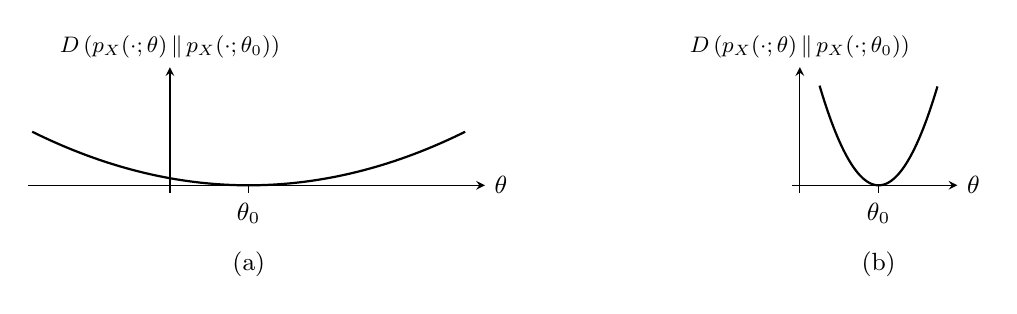
\begin{tikzpicture}
\shorthandoff{>}
%
\pgfmathsetmacro{\t}{1}
\pgfmathsetmacro{\dx}{8}
%
% peque�a curvatura
\draw[>=stealth,->] (-1.8,0)--(4,0) node[right]{\small $\theta$};
\draw[>=stealth,->] (0,-.1)--(0,1.5) node[above,scale=.9]
{\small $D\left( p_X(\cdot;\theta) \, \| \, p_X(\cdot;\theta_0) \right)$};
\draw[thick,domain=-1.75:3.75,samples=200] plot (\x,{.09*abs(\x-\t)^2});
\draw (\t,0)--(\t,-.1) node[below]{\small $\theta_0$};
%
% granda curvatura
\draw[>=stealth,->] ({-.1+\dx},0)--({2+\dx},0) node[right]{\small $\theta$};
\draw[>=stealth,->] (\dx,-.1)--(\dx,1.5) node[above,scale=.9]
{\small $D\left( p_X(\cdot;\theta) \, \| \, p_X(\cdot;\theta_0) \right)$};
\draw[thick,domain=.25:1.75,samples=200] plot ({\x+\dx},{2.25*abs(\x-\t)^2});
\draw ({\t+\dx},0)--({\t+\dx},-.1) node[below]{\small $\theta_0$};
%
\draw (\t,-1) node{\small (a)};
\draw ({\t+\dx},-1) node{\small (b)};
\end{tikzpicture} \end{center}
%
\leyenda{Ilustraci\'on         del        comportamiento         local        de
  $\Dkl[p_X(\cdot;\theta)]{p_X(\cdot;\theta_0)}$ \ en  funci\'on de \ $\theta$ \
  en \ $\theta_0$ \ en el contexto escalar \ $\Theta \subset \Rset$.  (a) Caso
  con \ $J_{\theta_0}(X)$  ``peque\~no'' \ y (b) caso  con \ $J_{\theta_0}(X)$ \
  ``grande''.   En  el caso  (b),  la determinaci\'on  de  \  $\theta$ \  usando
  $\Dkl{}$ \ va a  ser m\'as ``sencillo'' que en el caso  (a) porque el m\'inimo
  es m\'as ``picado''.}
%
\label{Fig:SZ:JCurvatura}
\end{figure}


% ================================= de Bruijn

\subseccion{Identidad de de Bruijn}
\label{Ssec:SZ:DeBruijn}


Un otro  v\'inculo entre el  mundo de la  informaci\'on y el de  la estimaci\'on
aparece a trav\'es de la identidad  de de Bruijn~\footnote{A pesar de que tom\'o
  este nombre, esta identidad en su primera versi\'on fue publicada por Stam. En
  su papel~\cite{Sta59}, menciona que  esta identidad fue comunicada al Profesor
  van  Soest por el  Profesor de  Bruijn.}~\cite{Sta59, CovTho06,  Joh04, Bar84,
  Bar86,  PalVer06, TorZoz18}.  Esta  identidad caracteriza  lo que  es conocido
como  canal gaussiano  de la  figura Fig~\ref{Fig:SZ:deBruijnVerdu}-(a),  \ie la
salida \ $Y$  \ es una versi\'on ruidosa de la  entrada.  La identidad v\'incula
las variaciones  de entrop\'ia  de salida con  respecto al  nivel de ruido,  y la
informaci\'on de Fisher.

\begin{figure}[h!]
%
\begin{center} 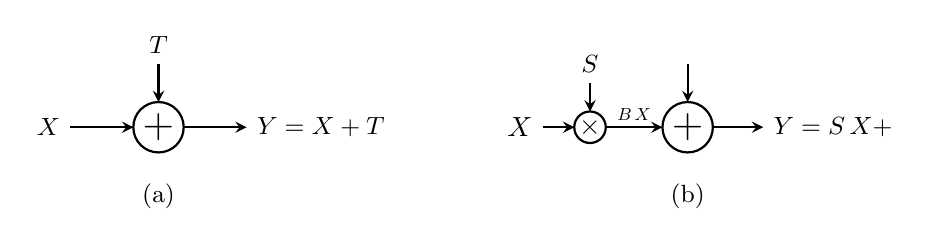
\begin{tikzpicture}[scale=.8]
\shorthandoff{>}
%
\begin{scope}
\draw[>=stealth,->,thick] (0,0) node[left]{\small $X$} --(1,0);
\draw[thick] (1.4,0) circle (.4);
\draw[>=stealth,->,thick] (1.4,1) node[above]{\small $T \N$} --(1.4,.4);
\node[align=center,scale=1.25] at (1.4,0){\large +};
\draw[>=stealth,->,thick] (1.8,0)--(2.8,0) node[right]{\small $Y = X + T \N$};
%
\end{scope}
%
\begin{scope}[xshift=7.5cm]
\draw[>=stealth,->,thick] (0,0) node[left]{$X$} --(.5,0);
\draw[thick] (.75,0) circle (.25);
\node[thick,align=center] at (.75,0){$\times$};
\draw[>=stealth,->,thick] (.75,.7) node[above]{\small $S$} --(.75,.25);
\draw[>=stealth,->,thick] (1,0)--(1.9,0);
\node[thick,align=center,scale=.7,above] at (1.45,0){\small $B \, X$};
\draw[thick] (2.3,0) circle (.4);
\draw[>=stealth,->,thick] (2.3,1) node[above]{\small $\N$} --(2.3,.4);
\node[align=center,scale=1.25] at (2.3,0){\large +};
\draw[>=stealth,->,thick] (2.7,0)--(3.5,0) node[right]{\small $Y = S \, X + \N$};
%
\end{scope}
\node at (1.4,-1.1){\small (a)};
\node at (9.8,-1.1){\small (b)};
\end{tikzpicture}
 \end{center}
%
\leyenda{Canal  de  comunicaci\'on  gaussiano  de  entrada  \  $X$.   (a)  Canal
  gaussiano usual, donde \ $T$ \ maneja los par\'ametros (nivel) del ruido.  (b)
  canal gaussiano con un preprocesamiento \ $S$ \ de la entrada.}
%
\label{Fig:SZ:deBruijnVerdu}
\end{figure}

\begin{teorema}[Identidad de de Bruijn]
\label{Teo:SZ:DeBruijn}
%
  Sea \ $X$ \  un vector aleatorio continuo sobre un abierto de  \ $\Rset^d$ \ y
  admitiendo una matriz de covarianza, y sea \ $Y = X + T \N$ \ donde \ $T$ \ es
  determinista, $d \times d'$ \ con \ $ d \le d'$, de rango m\'aximo, y \ $\N$ \
  un vector gaussiano centrado y de covarianza \ $\Sigma_\N$, independiente de \
  $X$   \  (ver   figura  Fig.~\ref{Fig:SZ:deBruijnVerdu}-(a)).    Entonces,  la
  entrop\'ia \modif{(diferencial)}  de Shannon y la  \modif{matriz informaci\'on
  no param\'etrica} de Fisher de \ $Y$ \ satisfacen
  %
  \[
  \nabla_T H(Y) = J(Y) \, T \, \Sigma_\N,
  \]
  %
  donde \ $\nabla_T \, \cdot$ \ es la matriz de componentes \ $\frac{\partial \,
    \cdot}{\partial T_{i,j}}$.  Si \ $T = T(\theta)$ \ depende de un par\'ametro
  escalar~\footnote{Si el  par\'ametro es  multivariado, hace falta  entender la
    desigualdad a trav\'es de derivas parciales con respecto a los componentes de
    $\theta$.}  $\theta$,
  %
  \[
  \frac{\partial}{\partial \theta}  H(Y) = \Tr\left( J(Y) \,  T \, \Sigma_\N
    \, \frac{\partial T^t}{\partial \theta} \right).
  \]
\end{teorema}
%
\begin{proof}
  La clave de este resultado viene del hecho que la densidad \ $p$ \ de \ $T \N$
  \ satisface una ecuaci\'on diferencial  particular.  La distribuci\'on de \ $T
  \N$  \ se  escribe \  $p(x) =  (2 \pi)^{-\frac{d}{2}}  \left| T  \Sigma_\N T^t
  \right|^{-\frac12}   \exp\left(  -   \frac12  x^t   \left(  T   \Sigma_\N  T^t
    \right)^{-1} x  \right)$ \ (el rango  m\'aximo de \  $T$ \ asegura que  \ $T
  \Sigma_\N  T^t$   \  sea  invertible).    Para  una  matriz   invertible  $R$,
  desarollando \  $|R|$ \  con respecto  a su l\'inea  \ $i$,  se obtiene  que \
  $\frac{\partial |R|}{\partial R_{i,j}} = R_{i,j}^*$ \ cofactor de \ $R_{i,j}$,
  dando  por la  regla de  Cram\'er \  $\nabla_R  |R| =  |R| \,  R^{-t}$ \  (ver
  tambi\'en~\cite[cap.~1~\&~9]{MagNeu99}), es decir \ $\nabla_R |R|^{-\frac12} =
  -\frac12 |R|^{-\frac12}  R^{-t}$.  De $\frac{\partial |R|^{-\frac12}}{\partial
    T_{i,j}}  =   \sum_{k,l}  \frac{\partial  |R|^{-\frac12}}{\partial  R_{k,l}}
  \frac{\partial R_{k,l}}{\partial T_{i,j}} = -\frac12 |R|^{-\frac12} \sum_{k,l}
  \left( R^{-1} \right)_{l,k} \frac{\partial R_{k,l}}{\partial T_{i,j}}$ \ con \
  $R  = T  \Sigma_\N  T^t$ \  (sim\'etrica)  y c\'alculos  b\'asicos se  obtiene
  finalmente
  %
  \[
  \nabla_T  \left|   T  \Sigma_\N  T^t  \right|^{-\frac12}  =   -  \left|  T
    \Sigma_\N T^t \right|^{-\frac12} \left( T \Sigma_\N T^t \right)^{-1}
  T \Sigma_\N.
  \]
  %
  Adem\'as, de \ $\left( T  \Sigma_\N T^t \right) \left( T \Sigma_\N T^t
  \right)^{-1}  =  I$ \  viene  \  $\frac{\partial  \left( T  \Sigma_\N  T^t
    \right)^{-1}}{\partial T_{i,j}} = -  \left( T \Sigma_\N T^t \right)^{-1}
  \frac{\partial \left( T \Sigma_\N  T^t \right)}{\partial T_{i,j}} \left( T
    \Sigma_\N T^t \right)^{-1}$.  Usando le vector \ $\uno_i$ \ con 1 en su \
  $i$-\'esima componente, y cero si no (ver notaciones), se obtiene
  %
  \begin{eqnarray*}
  \frac{\partial \left( x^t \left( T \Sigma_\N T^t \right)^{-1} x
  \right)}{\partial T_{i,j}} & = & - x^t \left( T \Sigma_\N T^t \right)^{-1}
  \left( \uno_i \uno_j^t \Sigma_\N T^t + T \Sigma_\N \uno_j \uno_i^t \right) \left( T
  \Sigma_\N T^t \right)^{-1} x\\[2.5mm]
  %
  & = & - 2 \, \uno_i^t \left( T \Sigma_\N T^t \right)^{-1} x x^t \left( T
  \Sigma_\N T^t \right)^{-1} T \Sigma_\N \uno_j
  \end{eqnarray*}
  %
  usando la relaci\'on  \ $x^t A \uno_k \uno_l^t B  x = \uno_l^t B x  x^t A \uno_k =
  \uno_k^t A^t x x^t  B^t \uno_l$ \ (escalares comutan y un  escalar es igual a su
  traspuesta) y usando la simetr\'ia de \ $T \Sigma_\N T^t$.  Eso significa
  que
  %
  \[
  \nabla_T \left( x^t \left( T \Sigma_\N T^t \right)^{-1} x \right) = - 2 \,
  \left(  T \Sigma_\N  T^t \right)^{-1}  x  x^t \left(  T \Sigma_\N  T^t
  \right)^{-1} T \Sigma_\N,
  \]
  %
  dando
  %
  \[
  \nabla_T p(x)  = \left( - \left(  T \Sigma_\N T^t \right)^{-1}  + \left( T
      \Sigma_\N  T^t   \right)^{-1}  x   x^t  \left(  T   \Sigma_\N  T^t
    \right)^{-1} \right) T \Sigma_\N \, p(x).
  \]
  %
  Tomando la Hessiana de \ $p$ \  con respecto a \ $x$ \ se obtiene sencillamente
  que \ $p$ \ satisface la ecuaci\'on diferencial
  %
  \[
  \nabla_T \, p = \Hess_x \, p \: T \, \Sigma_\N.
  \]
  %
  Suponiende que  se puede intervertir derivadas  y integrales (ver~\cite{Bar84,
    Bar86}     donde     se      dan     condiciones     rigurosas,     y     el
  teorema~\ref{Teo:MP:IntegralParametro},
  %pagina~\pageref{Teo:MP:IntegralParametro}),     
  $\displaystyle  p_Y(y)  =  \int_{\Rset^d}  p_X(x)  \, p(y-x)  \,  dx$  \  (ver
  ejemplo~\ref{Ej:MP:Suma})
  %,  pagina~\pageref{Ej:MP:Suma})
  \ satisface tambi\'en esta ecuaci\'on diferencial, y adem\'as
  %
  \begin{eqnarray*}
  \nabla_T H(Y) & = & - \int_{\Rset^d} \nabla_T \, p_Y(y) \log p_Y(y)
  \, dy - \int_{\Rset^d} \nabla_T \, p_Y(y) \, dy\\[2.5mm]
  %
  & = & - \left( \int_{\Rset^d} \Hess_y \, p_Y(y) \log p_Y(y) \, dy \right) T \,
  \Sigma_\N - \nabla_T \int_{\Rset^d} p_Y(y) \, dy\\[2.5mm]
  %
  & = & - \left( \int_{\Rset^d} \left( \Hess_y \Big( p_Y(y) \log p_Y(y) \Big) -
  \Hess_y \, p_Y(y) - \frac{\nabla_y \, p_Y(y) \, \nabla_y \, p_Y(y)^t}{p_Y(y)}
  \right) \, dy \right) T \, \Sigma_\N\\[2.5mm]
  %
  & = & - \left( \int_{\Rset^d} \Hess_y \Big( p_Y(y) \log p_Y(y) \Big) \, dy -
  \int_{\Rset^d} \Hess_y p_Y(y) \, dy \right) T \, \Sigma_\N \: + \: J(Y) \, T
  \, \Sigma_\N
  \end{eqnarray*}
  %
  usando la ecuaci\'on diferencial en la segunda l\'inea, el hecho que \ $p_Y$ \
  suma  a  1 en  la  tercera  l\'inea (su  gradiente  es  cero  entonces), y  la
  definici\'on de la matriz de Fisher  en la \'ultima l\'inea. Usando el teorema
  de la  divergencia (intergraci\'on por partes) aplicada  respectivamente a los
  componentes de \ $\nabla_y p_Y \log  p_Y$ \ y \ $\nabla_y p_Y$, suponiendo que
  estos gradientes se cancelan en el borde del dominio de integraci\'on, los dos
  t\'erminos integrales  valen cero, lo que  cierra la prueba  de la desigualdad
  general.  Adem\'as,  si \ $T =  T(\theta)$, la segunda desigualdad  sigue de \
  $\frac{\partial   \cdot}{\partial    \theta}   =   \sum_{i,j}   \frac{\partial
    \cdot}{\partial   T_{i,j}}   \frac{\partial   T_{i,j}}{\partial  \theta}   =
  \Tr\left( \nabla_T \cdot \, \frac{\partial T^t}{\partial \theta} \right)$.
\end{proof}

La versi\'on  inicial de la identidad de  de Bruijn, con \  $\Sigma_\N = I$,
que se escribe
%
\[
\frac{d}{d\theta}     H(X+\sqrt{\theta}    \N)    =     \frac12    \Tr\left(
  J(X+\sqrt{\theta} \N) \right),
\]
%
se recupera  en el caso particular  \ $T =  \sqrt{\theta} I$.  En este  caso, la
ecuac\'ion diferencial satisfecha por la densidad  de probabilidad \ $p$ \ es la
{\it  ecuaci\'on del  calor}.  Esta  desigualdad cuantifica  las  variaciones de
entrop\'ias   bajo  variaciones   de  ``niveles''   del  ruido   del   canal  de
comunicaci\'on. De una  forma, caracteriza la robustez del  canal con respecto al
nivel de ruido gaussiano (la gaussiana juega de nuevo un rol central ac\'a).

\

Existe una  otra forma  muy similar  de esta desigualdad  debido a  Guo, Shamai,
Verd\'u,  Palomar~\cite{GuoSha05, PalVer06,  TorZoz18}.  Esta  versi\'on vincula
a\'un m\'as el mundo  de la informaci\'on y el de la  estimaci\'on.  Del lado de
la  comunicaci\'on, consiste  a  caracterizar la  informaci\'on  mutua entre  la
entrada \ $X$ \ de un canal ruidoso y su  salida, \ $Y = S X + \N$ \ donde \
$S$ \ coresponde a un pre-tratamiento antes de la salida. Eso es ilustrado en la
figura  Fig.~\ref{Fig:SZ:deBruijnVerdu}-(b).  Del lado  de la  estimaci\'on, uno
puede querer  estimar \ $X$  \ observando solamente  \ $Y$.  Es conocido  que el
estimador  que minimiza  el error  cuadr\'atico promedio  \  $\Esp\left[ \left|
    \widehat{X}(Y)  - X  \right|^2 \right]$  \  es la  esperanza condicional  \
$\widehat{X}(Y)   =    \Esp[X|Y]$~\cite{Kay93,   Rob07,   LehCas98}.     \   Una
caracter\'istica de un  estimador siendo su matriz de  covarianza, se notar\'a \
$\E(X|Y)  =  \Esp\left[  \left( X  -  \Esp[X|Y]  \right)  \left( X  -  \Esp[X|Y]
  \right)^t  \right]$ \  esta  matriz.  Sorpredentemente,  existe tambi\'en  una
identidad entre \ $I(X;Y)$ \ y \ $\E(X|Y)$:
%
\begin{teorema}[Identidad de Guo--Shamai--Verd\'u]
\label{Teo:SZ:GuoShamaiVerdu}
%
  Sea \ $X$ \ un vector aleatorio  continuo sobre un abierto de \ $\Rset^{d'}$ \
  y admitiendo una  matriz de covarianza, y sea \  $Y = S X +  \N$ \ donde \
  $S$  es determinista,  $d  \times d'$,  y  \ $\N$  \  un vector  gaussiano
  centrado  y de covarianza  $\Sigma_\N$, independiente  de $X$  (ver figura
  Fig.~\ref{Fig:SZ:deBruijnVerdu}-(b)). Entonces, la informaci\'on mutua entre \
  $X$ \ e \ $Y$ \ y  la matriz de covarianza del estimador de error cuadr\'atico
  m\'inimo satisfacen
  %
  \[
  \nabla_S \, I(X;Y) = \Sigma_\N^{-1} S \, \E(X|Y).
  \]
  %
  Si \ $S = S(\snr)$ \ depende de un par\'ametro escalar $\snr$,
  %
  \[
  \frac{\partial}{\partial \snr} I(X;Y) = \Tr\left( \Sigma_\N^{-1} \, S \,
    \E(X|Y) \, \frac{\partial S^t}{\partial \snr} \right).
  \]
\end{teorema}
%
\begin{proof}
  Notando  que \ $p_{Y|X=x}  (y) =  (2 \pi)^{-\frac{d}{2}}  \left| \Sigma_\N
  \right|^{-\frac12}  \exp\left( -\frac12  (y-S  x)^t \Sigma_\N^{-1}  (y-Sx)
  \right)$   \   viene  \   $\nabla_S   \,   p_{Y|X=x}(y)   =  p_{Y|X=x}(y)   \,
  \Sigma_\N^{-1}  (y -  S x)  x^t$ \  (ver  unos pasos  de la  prueba de  la
  identidad de de  Bruijn) as\'i que \ $\nabla_y  \, p_{Y|X=x}(y) = p_{Y|X=x}(y)
  \, \Sigma_\N^{-1} (y - S x)$, dando
  %
  \[
  \nabla_S \, p_{Y|X=x}(y) = \nabla_y \, p_{Y|X=x}(y) x^t \qquad \mbox{y} \qquad
  \nabla_S \, p_{X,Y}(x,y) = \nabla_y \, p_{X,Y}(x,y) x^t
  \]
  %
  (multiplicando ambos lados por $p_X$). Ahora, \ $I(X;Y) = H(Y) - H(Y|X) = H(Y)
  - H(\N)$ \ (de la independencia, cuando \ $X  = x$, \ $Y = S x + \N$ \
  gaussiana de  misma convarianza que \  $\N$ \ y  de promedio \ $S  x$ (ver
  ejemplo~\ref{Ej:MP:SumaCond},
  % pagina~\pageref{Ej:MP:SumaCond}), 
  as\'i que
  %
  \begin{eqnarray*}
  \nabla_S I(X;Y) & = & \nabla_S H(Y)\\[2.5mm]
  %
  & = & - \int_{\Rset^d \times \Rset^{d'}} \nabla_S \Big( p_{X,Y}(x,y) \, \log
  p_Y(y) \Big) \, d\mu(x,y)\\[2.5mm]
  %
  & = & - \int_{\Rset^d \times \Rset^{d'}} \nabla_S \, p_{X,Y}(x,y) \, \log p_Y(y) \,
  d\mu(x,y) - \int_{\Rset^d \times \Rset^{d'}} p_{X|Y=y}(x) \, \nabla_S \, p_Y(y) \, d\mu(x,y)\\[2.5mm]
  %
  & = & \int_{\Rset^d \times \Rset^{d'}} \nabla_y \, p_{X,Y}(x,y) \, x^t \log p_Y(y)
  \, d\mu(x,y) - \int_{\Rset^d} \nabla_S \, p_Y(y) \, d\mu(y)\\[2.5mm]
  %
  & = & - \int_{\Rset^d \times \Rset^{d'}} \nabla_y \, p_Y(y) x^t p_{X|Y=y}(x) \, d\mu(x,y)\\[2.5mm]
  %
  & = & - \int_{\Rset^d} \nabla_y \, p_Y(y) \, \Esp\left[X^t | Y = y \right] \, d\mu(y)
  \end{eqnarray*}
  %
  La  segunda l\'inea  viene  de la  escritura  de \  $H(Y)$  usando $p_Y$  como
  marginale de $p_{X,Y}$ en $x$ y intercambiando gradiente e integral (ver pasos
  de   la   prueba  de   la   desigualdad  de   de   Bruijn);   la  tercera   de
  $\frac{p_{X,Y}(x,y)}{p_Y(y)}  =   p_{X|Y=y}(x)$;  en  la  cuarta   se  usa  la
  ecuaci\'on  diferencial satisfecha  por  $p_{X,Y}$ en  la  primera integral  y
  integrando en $x$ en la segunda  integral; la quinta l\'inea se obtiene usando
  el teorema de  la divergencia (intergraci\'on por partes)  en la integraci\'on
  en $y$  de la primera  integral, e intercambiando  gradiente e integral  el la
  segunda ($p_Y$ sumando a 1, el t\'ermino se cancela). Adem\'as,
  %
  \begin{eqnarray*}
  \nabla_y p_Y(y) & = & \int_{\Rset^{d'}} \nabla_y \, p_{Y|X=x}(y) \, p_X(x) \,
  d\mu(x)\\[2.5mm]
  %
  & = & - \Sigma_\N^{-1} \int_{\Rset^{d'}} (y - S x) \, p_{Y|X=x}(y) \, p_X(x) \,
  d\mu(x)\\[2.5mm]
  %
  & = & - \Sigma_\N^{-1} \left( y - S \int_{\Rset^{d'}} x \, p_{X|Y=y}(x) \,d\mu(x)
  \right) p_Y(y)\\[2.5mm]
  %
  & = & - \Sigma_\N^{-1} \Big( y - S \Esp\left[X | Y=y \right] \Big) \, p_Y(y)
  \end{eqnarray*}
  %
  escribiendo $p_{Y|X=x}(y)  \, p_X(x) =  p_{X|Y=y}(x) \, p_Y(y)$ en  la tercera
  l\'inea. Esta ecuaci\'on permite escribir
  %
  \begin{eqnarray*}
  \nabla_S I(X;Y) & = & \Sigma_\N^{-1} \int_{\Rset^d} \Big( y - S \Esp\left[X |
  Y=y \right] \Big) \Esp\left[X^t | Y=y \right] \, p_Y(y) \, d\mu(y)\\[2.5mm]
  %
  & = & \Sigma_\N^{-1} \left( \Esp\left[ Y \Esp\left[ X^t|Y \right] \right] - S
  \Esp\left[ \Esp\left[X | Y \right] \Esp\left[X | Y \right]^t \right]
  \right)\\[2.5mm]
  %
  & = & \Sigma_\N^{-1} \left( \Esp\left[ Y X^t \right] - S \Esp\left[
  \Esp\left[X | Y \right] \Esp\left[X | Y \right]^t \right] \right)\\[2.5mm]
  %
  & = & \Sigma_\N^{-1} S \left( \Esp\left[ X X^t \right] - \Esp\left[
  \Esp\left[X | Y \right] \Esp\left[X | Y \right]^t \right] \right)
  \end{eqnarray*}
  %
  la \'ultima l\'inea viniendo de $Y  = S X + \N$ con $\N$ independiente
  de  $X$ y  de  promedio 0.   La prueba  se  cierra notando  que \  $\Esp\left[
    \Esp[X|Y] \right]  = \Esp[X]$  \ y por  la f\'ormula de  K\"onig-Huyggens (ver
  cap\'itulo~\ref{cap:MP:TeoriaProbabilidades},
  subsecci\'on~\ref{Ssec:MP:Momentos}).
  % , pagina~\pageref{Ssec:MP:Momentos}).

  La  segunda identidad  viene de  \ $\frac{\partial  \cdot}{\partial  \snr} =
  \Tr\left(  \nabla_S \,  \frac{\partial S^t}{\partial  \snr} \right)$  \ (ver
  prueba de la identidad de de Bruijn).
\end{proof}
%
\noindent  La  primera versi\'on  de  esta  identidad se  recupera  con  \ $S  =
\sqrt{\snr}$, \ $\Sigma_\N = I$ \ y \ $X$ \ de covarianza la identidad; $\snr$ \
es conocido como relaci\'on se\~nale/ruido en este caso.

Existen versiones a\'un m\'as completas  (con gradientes con respecto a la matriz
\  $\Sigma_\N$  \  por  ejemplo)  que se  pueden  consultar  en~\cite{Joh04,
  PalVer06, PayPal09}.



% ================================= Stam

\subseccion{Desigualdad de Stam}
\label{Ssec:SZ:Stam}


De la  desigualdad de  la potencia entr\'opica  y de  la identidad de  de Bruijn
surge  una otra  desigualdad implicando  la potencia  entr\'opica \  $N$ \  y la
informaci\'on de Fisher \ $J$.  Esta desigualdad es conocida como desigualdad de
Stam~\footnote{Como para  la identidad  de de Bruijn,  Stam mencion\'o  que esta
  desigualdad fue  comunicada al  Profesor van Soest  por el Profesor  de Bruijn
  quien  da una  prueba variacional  de la  desigualdad.}~\cite{CovTho06, Rio07,
  Sta59},     o    a    veces     ``desigualdad    isoperimetrica     para    la
entrop\'ia''~\cite{WanMad04}.
%
\begin{teorema}[Desigualdad de Stam]
\label{Teo:SZ:Stam}
%
  Sea  \  $X$   \  una  variable  aleatoria  continua   sobre  \  $\X  \subset
  \Rset^d$. Entonces,
  %
  \[
  N(X) \Tr\left( J(X) \right) \, \ge \, d,
  \]
  %
  con igualdad si y solamente si \ $X$ \ es gaussiano de covarianza proporcional
  a la identidad.
\end{teorema}
%
\begin{proof}
  De la desigualdad de la potencia entr\'opica se obtiene \ $N(X + \sqrt{\theta}
  \N)  \ge N(X)  + \theta  \left| \Sigma_\N  \right|^{\frac1d}$. Tomando
  $\Sigma_\N =  I$, se  obtiene \ $\forall  \, \theta  > 0,$ \  $\frac{N(X +
    \sqrt{\theta} \N) - N(X)}{\theta}  \ge 1$.  Entonces, tomando el l\'imite
  \ $\theta \to 0$, aparece  que \ $\left. \frac{d}{d\theta} N(X + \sqrt{\theta}
    \N)   \right|_{\theta  =   0}  \ge   1$.   La   prueba  se   cierra  con
  $\frac{d}{d\theta}  N(X   +  \sqrt{\theta}   \N)  =  \frac{1}{2   \pi  e}
  \frac{d}{d\theta}  \exp\left( \frac2d  H(X +  \sqrt{\theta} \N)  \right) =
  \frac2d  N(X +  \sqrt{\theta}  \N) \frac{d}{d\theta}  H(X +  \sqrt{\theta}
  \N) = d N(X +  \sqrt{\theta} \N) \Tr\left( J(X + \sqrt{\theta} \N)
  \right)$ \ (por la identidad de  de Bruijn).  Adem\'as, la igualdad se obtiene
  cuando se  alcanza la cota  de la desigualdad  de la potencia  entr\'opica, es
  decir cuando \ $X$ \ es gaussiano de varianza proporcional a la del ruido, que
  es la identidad en este caso.
\end{proof}
%
Se  puede  ver  de  nuevo  el  rol  central  que  juega  la  gaussiana  en  esta
desigualdad. Adem\'as, de la desigualdad  de Stam se puede deducir tamb\'ien las
versiones escalares de la desigualdad de Cram\'er-Rao. Viene del hecho que, dada
una matriz de covarianza, la entrop\'ia \ $H(X)$ \ es m\'axima cuando \ $X$ \ es
gaussiano.  Entonces, para cualquier \ $X$ \ de covarianza \ $\Sigma_X$, \ $N(X)
\le  \left| \Sigma_X  \right|^{\frac1d}$,  dando  de la  desiguldad  de Stam,  \
$\left| \Sigma_X \right|^{\frac1d} \Tr\left( J(X)  \right) \ge d$ \ (y las otras
versiones  escalares de  la relaci\'on  determinente-traza).  Como  se  lo puede
esperar, se  obtiene la igualdad si y  solamente \ $X$ \  es gaussiano (potencia
entr\'opica alcanzando su  cota superior) y de matriz  la identidad (desiguladad
de Stam se saturando).

Varias   otras  pruebas   de  la   desigualdad  de   Stam  pueden   provenir  de
generalizaciones~\cite{Ber12:06_1, Ber13, LutYan05, LutLv12, ZozPue17}.
%, por ejemplo debido a Lutwak o Bercher~\cite{Lut, Ber}.
  \SZ{La
  secci\'on ZZZ lo va a rapidamente evocar. Ver caso discreto Kagan~\cite{Kag01}.}


% ========================= Ejemplos & Aplicaciones ========================== %

\seccion{Unos ejemplos y aplicaciones}
\label{Sec:SZ:Ejemplos}


% ================================= canal

\subseccion{Canal de transmisi\'on y su capacidad}
\label{Ssec:SZ:CanalCapacidad}

Siguiendo el  esquema de comunicaci\'on de  Shannon, un mensaje  que se modeliza
como  un vector  aleatorio~\footnote{De  punto  de vista  de  un receptor,  este
  mensaje es  desconocido. Adem\'as, se lo  puede ver como una  instancia de una
  clase  importante   de  posibles  mensajes,   justificando  la  modelizaci\'on
  aleatoria.} $X$  pasa por un  canal de comunicaci\'on  y se recibe  un mensaje
$Y$, vector  aleatorio. En el trabajo de  Shannon, el canal es  supuesto a ruido
aditivo,  es decir  que se  a\~nade un  ruido a  $X$.  De  manera  general, para
conocer la informaci\'on de $X$ que se recibe, se calcula la informaci\'on mutua
$I(X;Y)$, es  decir la cantidad de  informaci\'on que comparten la  entrada y la
salida  del  canal.  Lo  m\'as  $I$  es grande,  lo  m\'as  de informaci\'on  se
transmite.  Dado el canal, se puede arreglar $X$ (su distribuci\'on) de manera a
maximizar $I(X;Y)$,  es decir  la cantidad m\'axima  que se puede  transmitir en
este    canal.    Es    lo     que    es    conocido    como    capacidad    del
canal~\cite[part.~II~\&~III]{Sha48} (ver  tambi\'en~\cite{CovTho06, Rio07} entre
otros):
%
\begin{definicion}[Capacidad de canal]
\label{Def:SZ:CapacidadCanal}
%
  Sea un canal de transmisi\'on, $X$  su entrada e $Y$ su salida, como ilustrado
  figura  Fig.~\ref{Fig:SZ:CanalComunicacion}.  Sea  $p_X$ la  distribuci\'on de
  probabilidad de $X$. La capacidad $C$ del canal es definida por
  %
  \[
  C = \max_{p_X} \, I(X;Y).
  \]
\end{definicion}

\begin{figure}[h!]
%
\begin{center} 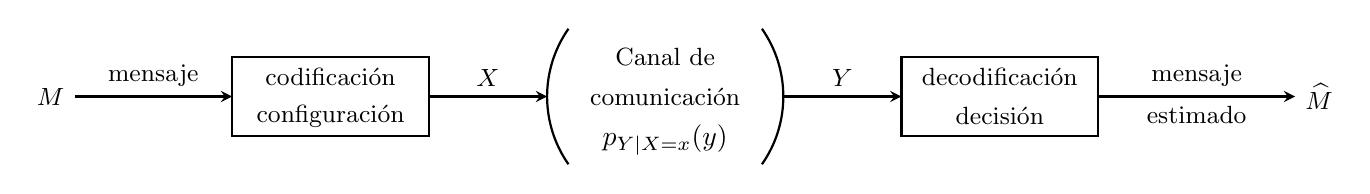
\begin{tikzpicture}
\shorthandoff{>}
%
% Mensaje
\draw[>=stealth,->,thick] (0,0) node[left]{\small $M$} --(2,0);
\node[above] at (1,0){\small mensaje};
%
% codificacion
\draw[thick] (2,-.5) rectangle (4.5,.5);
\node at (3.25,.25){\small codificaci\'on};
\node at (3.25,-.25){\small configuraci\'on};
%
% entrada del canal
\draw[>=stealth,->,thick] (4.5,0)--(6,0);
\node[above] at (5.25,0){\small $X$};
%
% Canal de com
\pgfmathsetmacro{\t}{35};
\pgfmathsetmacro{\r}{1.5};
\draw[thick] ({6+\r*(1+cos(180-\t))},{\r*sin(\t)}) arc (180-\t:180+\t:\r);
\draw[thick] ({6+\r*(1+cos(\t))},{-\r*sin(\t)}) arc (-\t:\t:\r);
\node at ({6+\r},.5){\small Canal de};
\node at ({6+\r},0){\small comunicaci\'on};
\node at ({6+\r},-.55){$p_{Y|X=x}(y)$};
%
% salida
\draw[>=stealth,->,thick] ({6+2*\r},0)--({7.5+2*\r},0);
\node[above] at ({6.75+2*\r},0){\small $Y$};
%
% decodificacion/decision
\draw[thick] ({7.5+2*\r},-.5) rectangle ({10+2*\r},.5);
\node at ({8.75+2*\r},.25){\small decodificaci\'on};
\node at ({8.75+2*\r},-.25){\small decisi\'on};
%
% Mensaje estimado
\draw[>=stealth,->,thick] ({10+2*\r},0)--({12.5+2*\r},0) node[right]{\small $\widehat{M}$};
\node[above] at ({11.25+2*\r},0){\small mensaje};
\node[below] at ({11.25+2*\r},0){\small estimado};
\end{tikzpicture}
 \end{center}
%
\leyenda{Esquema de comunicaci\'on de Shannon.  En una primera etapa, un mensaje
  $M$ a  transmitir es  c\'odificado (ej.  c\'odigo  binario) o puesto  en forma
  (ej.  s\'imbolos  modulando una  funci\'on para que  sea anal\'ogica y  en una
  banda  de frecuencias  dada).  Sea  $X$ este  mensaje codificado  o  puesto en
  forma.  A la  recepci\'on, se mide $Y$ (ej.  versi\'on  ruidosa de $X$), antes
  de ser decodificado o usado para tomar una decisi\'on, $\widehat{M}$ siendo la
  estimaci\'on de  $M$ (ej.  s\'imbolos estimados  a partir de  $Y$).  Una etapa
  importante es el v\'inculo entre la entrada  $X$ y la salida $Y$ del canal, es
  decir la  cantidad de informaci\'on que  tienen en com\'un.   La capacidad del
  canal es la informaci\'on $I(X;Y)$ m\'axima con respeto a su entrada.}
\label{Fig:SZ:CanalComunicacion}
\end{figure}


% ================================= canal binario

\subsubseccion{Canal binario}
\label{Sssec:SZ:CanalBinario}

Suponiendo  que el  mensaje mandado  en un  canal es  una cadena  de s\'imbolos,
variables   aleatorias  independientes,   se  puede   concentrarse   sobre  cada
s\'imbolo. En este marco, un canal de comunicaci\'on lo m\'as simple es conocido
como  {\it canal  binario}~\cite[Sec.~15]{Sha48}: $X$  es una  variable definida
sobre $\X =  \{ 0 \, , \, 1  \}$; tal tipo de entrada es  natural, pensando a la
codificaci\'on  binaria.  La  salida $Y$  es tambi\'en  definida sobre  $\X$; se
puede imaginar medir y tomar una decisi\'on binaria usando la medida.  Tal canal
es  definido por  sus  probabilidaded de  transici\'on  $p_{Y|X=x}(y)$, \ie  las
probabilidades que un 0 (resp. un 1) se transmite correctamente o cambia en un 1
(resp. 0), \ie
%
\[
\varepsilon = P(Y  = 1 | X =  0) = 1 - P(Y  = 0 | X = 0)  \qquad \mbox{y} \qquad
\vartheta = P(Y = 0 | X = 1) = 1 - P(Y = 1 | X = 1).
\]
%
$\varepsilon$ y $\vartheta$ representan errores de comunicaci\'on.  Tal canal es
descrito      figura     Fig.~\ref{Fig:SZ:CanalBinario}-(a).       La     figura
Fig.~\ref{Fig:SZ:CanalBinario}-(b) da un esquema ``pr\'actico'' que podr\'ia ser
al origen  de un  tal canal.  Cuando  \ $\varepsilon  = \vartheta$, el  canal es
conocido como {\it canal binario sim\'etrico}.  Cuando \ $\varepsilon = 0$ \ y \
$\vartheta \in (0 \; 1)$, el canal es conocido como {\it canal binario en Z}.

\begin{figure}[h!]
\begin{center} 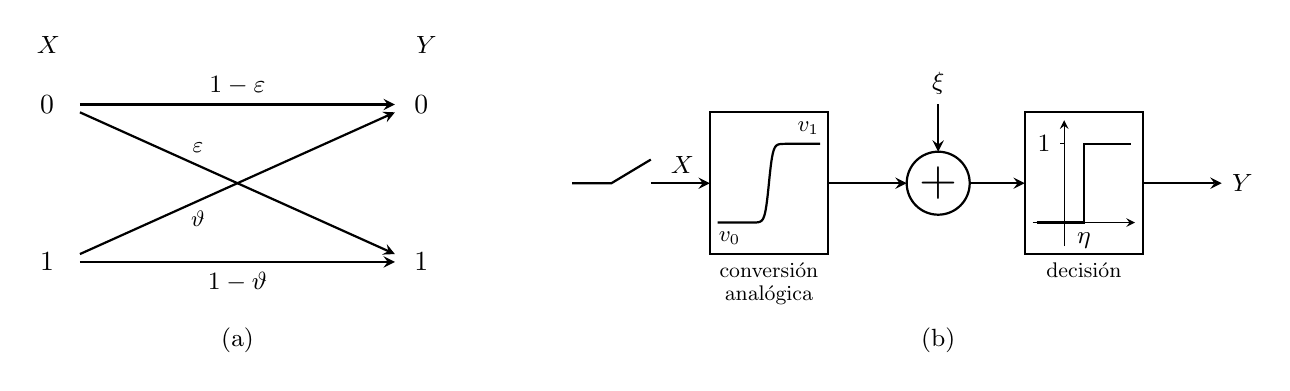
\begin{tikzpicture}
\shorthandoff{>}
%
\begin{scope}
\node at  (-.4,1.75){\small $X$}; \node at  (4.4,1.75){\small $Y$};
%
\draw[>=stealth,->,thick] (-.2,1) node[left]{0} (0,1) -- (4,1) node[right]{\ 0};
\node[above] at (2,1){\small $1-\varepsilon$};
%
\draw[>=stealth,->,thick] (-.2,-1) node[left]{1} (0,-1) -- (4,-1) node[right]{\ 1};
\node[below] at (2,-1){\small $1-\vartheta$};
%
\draw[>=stealth,->,thick] (0,.9)--(4,-.9);
\node[scale=.9] at (1.5,.45){\small $\varepsilon$};
%
\draw[>=stealth,->,thick] (0,-.9)--(4,.9);
\node[scale=.9] at (1.5,-.45){\small $\vartheta$};
%
\end{scope}
%
\begin{scope}[xshift=7cm]
%
% entrada
\draw[thick] (-.75,0)--(-.25,0)--(.25,.3);
\draw[>=stealth,->,thick] (.25,0)--(1,0);
%\draw[>=stealth,->,thick] (.25,-.5) node[below]{\small $X$} --(.25,.1);
\node[above] at (.65,0){\small $X$};
%
% puesta en niveles
\draw[thick] (1,-.9) rectangle (2.5,.9);
\node[scale=.9] at (1.25,-.7){\small $v_0$};
\node[scale=.9] at (2.25,.7){\small $v_1$};
\draw[thick,domain=-4.5:4.5,samples=100] (1.1,-.5) -- plot ({\x/10+1.75},{.5*tanh(2*\x)}) --(2.4,.5);
\node[below,scale=.85] at (1.75,-.9){\small conversi\'on};
\node[below,scale=.85] at (1.75,-1.2){\small anal\'ogica};
%
% adicion del ruido
\draw[>=stealth,->,thick] (2.5,0)--(3.5,0);
\draw[thick] (3.9,0) circle (.4);
\draw[>=stealth,->,thick] (3.9,1) node[above]{\small $\xi$} --(3.9,.4);
\node[align=center,scale=1.5] at (3.9,0){\large +};
%
% decision
\draw[>=stealth,->,thick] (4.3,0)--(5,0);
\draw[thick] (5,-.9) rectangle (6.5,.9);
\draw[>=stealth,->] (5.1,-.5)--(6.4,-.5);
\draw[>=stealth,->] (5.5,-.8)--(5.5,.8);
\draw[thick] (5.15,-.5)--(5.75,-.5)--(5.75,.5)--(6.35,.5);
\node[below] at (5.75,-.5){\small $\eta$};
\draw (5.5,.5)--(5.45,.5) node[left]{\small 1};
\node[below,scale=.85] at (5.75,-.9){\small decisi\'on};
%
% salida
\draw[>=stealth,->,thick] (6.5,0)--(7.5,0) node[right]{\small $Y$};
\end{scope}
\node at (2,-2){\small (a)};
\node at (10.9,-2){\small (b)};
\end{tikzpicture}
 \end{center}
%
\leyenda{(a): Canal binario.  La entrada $X$ definida  sobre $\X = \{ 0  \, , \,
  1\}$ pasa  por este canal  e $Y$  definida sobre $\Y  = \X$ es  recibido. Este
  canal es caracterizado por  las probabilidades de transici\'on $p_{Y|X=x}(y)$.
  (b): Esquema  que puede conducir al  canal binario; una variable  puede ser la
  salida de una puerta l\'ogica, con niveles $v_0$ (nivel bajo, codificando 0) y
  $v_1$  (nivel alto, codificando  1).  Se  puede imaginar  que este  voltaje es
  transmitido por un  canal a\~nandiendo un ruido $\xi$.   En la recepci\'on, se
  toma una  decisi\'on, por ejemplo  0 (resp.  1)  si la medida es  mayor (resp.
  menor)  que  $\eta  =   \frac{v_0  +  v_1}{2}+\Esp[\xi]$.   En  este  ejemplo,
  $\varepsilon$ \ y  \ $\vartheta$ \ van a  ser caracterizados completamente por
  la distribuci\'on  del ruido (y  de los dos  niveles posibles de  la entrada),
  pero no de la distribuci\'on $p_X$.}
\label{Fig:SZ:CanalBinario}
\end{figure}

En este caso, trabajando con bits, aparece leg\'itimo usar el logaritmo de base
2. Luego, sean
%
\[
r = P(X = 0),
\]
%
dando la distribuci\'on  de la entrada. La distribuci\'on de la  salida va a ser
dada a partir de $s = P(Y = 0) = P(Y = 0 | X = 0) P(X = 0) + P(Y = 0 | X
= 1) P(X = 1)$ es decir
%
\[
s = P(Y  = 0) = \vartheta +  r (1-\varepsilon-\vartheta).
\]
%
La informaci\'on  mutua se escribe  \ $I_2(X;Y) =  H_2(Y) - H_2(Y|X) =  H_2(Y) -
H_2(Y|X=0) P(X = 0) + H_2(Y|X=1) P(X = 1)$, lo que toma la expresi\'on
%
\[
I_2(X;Y) = h_2(s) - r h_2(\varepsilon) - (1-r) h_2(\vartheta),
\]
%
donde $h_2(u) = -  u \log_2 u - (1-u) \log_2 (1-u)$  es la entrop\'ia binaria en
bits.  Para calcular la capacidad $C_2$  en bits, hace falta maximizar $I_2$ con
respeto   a   $r$.    Diferenciando    $I_2$   en   $r$,   \ie   $\frac{\partial
  I_2(X;Y)}{\partial  r}  =  \frac{\partial h_2(s)}{\partial  s}  \frac{\partial
  s}{\partial r} - h_2(\varepsilon) + h_2(\vartheta)$, es decir
%
\[
\frac{\partial I_2(X;Y)}{\partial  r} = (1-\varepsilon-\vartheta)  \log_2 \left(
  \frac{1-s}{s} \right) - h_2(\varepsilon) + h_2(\vartheta).
\]
%
\begin{itemize}
\item Claramente,
  %
  \[
  \vartheta = 1-\varepsilon \quad \Rightarrow \quad C_2 = 0.
  \]
  %
  Viene del hecho  que para $\vartheta = 1-\varepsilon$,  de $h_2(\varepsilon) =
  h_2(1-\varepsilon)$ se deduce que $I_2(X;Y)  = 0$ constante. De hecho, en este
  caso, un 0 en la salida puede venir  de un 0 o 1 con probabilidades iguales, y
  lo mismo para  un 1 en la  salida; en otros t\'erminos, la  salida aparece ser
  independiente de la entrada.  Eso se verifica formalmente con $s = \vartheta$,
  dando $p_{Y|X=x}  = p_Y$, dando una  informaci\'on mutua nula,  y entonces una
  capacidad nula.
%
\item Si $\vartheta  \ne 1-\varepsilon$, la derivada de $I_2$  con respeto a $r$
  se anula para $s = s^\opt$ ($r = r^\opt$),
  %
  \[
  s^\opt = \frac{1}{1 +  2^{\frac{h(\varepsilon) - h(\vartheta)}{1 - \varepsilon
        -  \vartheta}}}  \qquad \mbox{siendo}  \qquad  r^\opt  = \frac{s^\opt  -
    \vartheta}{1 - \varepsilon - \vartheta},
  \]
  %
  y  dando   un  extremo   para  $I_2$.   A   continuaci\'on,  $\frac{\partial^2
    I_2}{\partial  r^2} = \frac{(1-\varepsilon-\vartheta)^2}{s  (1-s)} >  0$ (en
  particular para el $s$ ``\'optimo''),  probando que el extremo es un m\'aximo.
  Poniendo  la expresi\'on de  $r^\opt$ en  la formula  de $I_2(X;Y)$,  luego de
  muchos c\'alculos (b\'asicos), se obtiene
  %
  \[
  C_2  =  \log_2\left(  1  +  2^{\frac{h_2(\varepsilon)  -  h_2(\vartheta)}{1  -
        \varepsilon   -  \vartheta}}   \right)  -   \frac{(1  -   \vartheta)  \,
    h_2(\varepsilon)  -   \varepsilon  \,  h_2(\vartheta)}{1   -  \varepsilon  -
    \vartheta}.
  \]
  %
  Cuando  $\vartheta   \to  1-\varepsilon$,  notando   que  $h_2(\varepsilon)  =
  h_2(1-\varepsilon)$ y  tomando el  l\'imite de esta  formula, se  recupera que
  $C_2 \to 0$.
  %
  % ---
  %
  % \newline{\color{red}\bf �Interpretacion?  no hay combinacion convexa
  %   $\frac{\varepsilon}{1-\varepsilon-\vartheta}$ siendo del mismo signo que
  %   $\frac{1-\vartheta}{1-\varepsilon-\vartheta}$; nota: $C
  %   = \log_2\left( 1 + 2^{-
  %       \frac{h(1-\vartheta)-h(\varepsilon)}{(1-\vartheta)-\varepsilon}}
  %   \right) + \frac{1}{\varepsilon
  %     (1-\vartheta)} \frac{(1-\vartheta) h(1-\vartheta) - \varepsilon
  %     h(\varepsilon)}{\vartheta - (1-\varepsilon)}$}
\end{itemize}
%
\noindent De  \ $I_2(X;Y) = H_2(Y)  - H_2(Y|X) \le H_2(Y)  \le 1$ bit  \ ($Y$ es
binario, de entrop\'ia m\'axima en el caso uniforme), aparece sin c\'alculos que
%
\[
C_2 \le 1 \: \mbox{bit},
\]
%
\ie  la capacidad  es menor  que 1  bit: para  transmitir informaci\'on  en este
canal, hace falta introducir redundancia en  el mensaje.  Se alcanza \ $C_2 = 1$
bit si, (i) por  un lado $H_2(Y|X) = 0$, es decir  \ $r h_2(\varepsilon) + (1-r)
h_2(\vartheta) = 0$ \ y adem\'as (ii) \ $h_2(s) = 1$.  Estudiando cada caso (ej.
con \ $r = 0$ \ y \ $\vartheta =  0$ \ se satisface (i) pero no (ii) porque \ $s
= 0$), se obtiene que
%
\[
C_2  =  1  \qquad  \Leftrightarrow  \qquad  r =  \frac12  \quad  \mbox{y}  \quad
\varepsilon = \vartheta = \frac{1 \pm 1}{2}.
\]
%
Para  $\varepsilon =  \vartheta =  0$ el  canal es  perfecto, mientras  que para
$\varepsilon =  \vartheta =  1$ el  canal es llamado  {\it canal  volteando}; en
ambos casos, se recupera la entrada (o directamente, o tomando el opuesto) ``sin
perdida''.

La  figura  Fig.~\ref{Fig:SZ:ICanalBinario}  representa la  informaci\'on  mutua
$I(X;Y)$ para unos  canales ($\varepsilon$ y $\vartheta$ dados)  en funci\'on de
$r$.  Se nota que la curva es c\'oncava y tiene un m\'aximo \'unico~\footnote{De
  manera general, de la escritura de $I$ con entrop\'ias condicionales, para $X$
  definido sobre $\X$ e  $Y$ sobre $\Y$, da \ $0 \le C \le  \min( \log |\X| \, ,
  \, \log |\Y|  )$.  \ Adem\'as, $p_{Y|X=x}$  depende solo del canal y  no de la
  entrada, as\'i que  para \ $p_X =  \pi_1 p_{(1)} + \pi_2 p_{(2)}$  \ ($\pi_2 =
  1-\pi_1$) se obtiene \ $p_Y = \pi_1 q_{(1)} + \pi_2 q_{(2)}$ \ con \ $q_{(i)}$
  \ distribuci\'on de la salida corespondiente a una entrada de distribuci\'on \
  $p_{(i)}$.   Ahora, de  $I(X;Y) =  H(Y)-H(Y|X)$, el  segundo  t\'ermino siendo
  dependiente solamente del canal, de la concavidad de $H$ se obtiene de que $I$
  es c\'oncava con respeto a  $p_X$.  A continuaci\'on, $p_X$ parteneciendo a un
  convexo,  $I$ tiene un  m\'aximo que  es \'unico.},  capacidad del  canal.  La
figura  Fig.~\ref{Fig:SZ:CCanalBinario}  representa la  capacidad  del canal  en
funci\'on  de  \   $\varepsilon$  \  y  \  $\vartheta$   as\'i  que  unos  casos
particulares/cortes.

En  el caso  particular  $\varepsilon  = \vartheta$,  conocido  como {\it  canal
  sim\'etico}, la capacidad es
%
\[
C_2 = 1 - h_2(\varepsilon)
\]
%
(alcanzada  con  una entrada  uniforme).   Como visto  en  el  caso general,  la
capacidad vale 1  bit si y solamente si  \ $h_2(\varepsilon) = 0$, \  es decir \
$\varepsilon = 0$ \ o \ $\varepsilon = 1$.  Al rev\'es, la capacidad es m\'inima
cuando $H_2$ est m\'aximo, es decir  para \ $\varepsilon = \vartheta = \frac12$,
\ y  \ $C_2 = 0$  \ (instancia particular  de \ $\vartheta =  1-\varepsilon$). \
$h_2(\varepsilon)$  \  es la  perdida  en bit  para  cada  bit transmitido.   La
capacidad  \  $C_2$   \  en  funci\'on  de  \   $\varepsilon$\  es  dada  figura
Fig.~\ref{Fig:SZ:CCanalBinario}-(b).

En el  caso particular  $\varepsilon = 0$,  conocido como  {\it canal en  Z}, la
capacidad es
%
\[
C_2 = \log_2\left( 1 +  2^{- \frac{h_2(\vartheta)}{1-\vartheta}} \right).
\]
%
Se nota  en este caso tambi\'en  que la capacidad  alcanza 1, su m\'aximo,  si y
solamente  si \  $\vartheta  = 0$  \  (canal perfecto).   Al  rev\'es, cuando  \
$\vartheta  \to 1$,  \  $C \to  0$, \  instancia  particular de  \ $\vartheta  =
1-\varepsilon$.   La capacidad \  $C_2$ \  en funci\'on  de $\vartheta$  es dada
figura Fig.~\ref{Fig:SZ:CCanalBinario}-(c).

%{\bf\color{red} C parecido a la de Shannon caso continuo. Interpretacion?}

\begin{figure}[h!]
%
\begin{center} \begin{tikzpicture}[scale=2]
\shorthandoff{>}
%
%
% ----- Canal general
%
\begin{scope}
\pgfmathsetmacro{\p}{.4};% varepsilon
\pgfmathsetmacro{\q}{.01};% vartheta
%
\pgfmathsetmacro{\dpr}{1-\p-\q};
\pgfmathsetmacro{\hp}{-\p*log2(\p)-(1-\p)*log2(1-\p)};% h(varepsilon)
\pgfmathsetmacro{\hq}{-\q*log2(\q)-(1-\q)*log2(1-\q)};% h(vartheta)
\pgfmathsetmacro{\dh}{\hp-\hq};
%
\pgfmathsetmacro{\bopt}{1/(1+(2^((\hp-\hq)/\dpr)))};% s opt
\pgfmathsetmacro{\aopt}{(\bopt-\q)/\dpr};% r opt
\pgfmathsetmacro{\Capa}{-log2(\bopt)-((1-\q)*\hp-\p*\hq)/\dpr};
%
\draw[>=stealth,->] (-.2,0)--(1.2,0) node[right]{\small $r$};
\draw[>=stealth,->] (0,-.2)--(0,1.2) node[above]{\small $I_2(X;Y)$};
%
\draw[thick,domain=0:1,samples=100] (0,0)-- plot (\x,
{-(\q+\dpr*\x)*log2(\q+\dpr*\x)-(1-\q-\dpr*\x)*log2(1-\q-\dpr*\x)-\x*\hp-(1-\x)*\hq)})
--(1,0);
%
\draw (\aopt,0)--(\aopt,-.05) node[below]{\small $r^\opt$};
\draw (1,0)--(1,-.05) node[below]{\small 1};
\draw (0,\Capa)--(-.05,\Capa) node[left]{\small $C_2$};
\draw (0,1)--(-.05,1) node[left]{\small 1};
\end{scope}
%
%
% ----- Canal simetrico
%
\begin{scope}[xshift=2.5cm]
\pgfmathsetmacro{\p}{.05};
%
\pgfmathsetmacro{\dpr}{1-2*\p};
\pgfmathsetmacro{\hp}{-\p*log2(\p)-(1-\p)*log2(1-\p)};
%
\pgfmathsetmacro{\Capa}{1-\hp};
%
\draw[>=stealth,->] (-.2,0)--(1.2,0) node[right]{\small $r$};
\draw[>=stealth,->] (0,-.2)--(0,1.2) node[above]{\small $I_2(X;Y)$};
%
\draw[thick,domain=0:1,samples=100] (0,0)-- plot (\x,
{-(\p+\dpr*\x)*log2(\p+\dpr*\x)-(1-\p-\dpr*\x)*log2(1-\p-\dpr*\x)-\hp)})
--(1,0);
%
\draw (.5,0)--(.5,-.05) node[below]{\small $r^\opt$};
\draw (1,0)--(1,-.05) node[below]{\small 1};
\draw (0,\Capa)--(-.05,\Capa) node[left]{\small $C_2$};
\draw (0,1)--(-.05,1) node[left]{\small 1};
\end{scope}
%
%
% ----- Canal en Z
%
\begin{scope}[xshift=5cm]
\pgfmathsetmacro{\q}{.3};
%
\pgfmathsetmacro{\dpr}{1-\q};
\pgfmathsetmacro{\hq}{-\q*log2(\q)-(1-\q)*log2(1-\q)};
%
\pgfmathsetmacro{\bopt}{1/(1+(2^(-\hq/\dpr)))};
\pgfmathsetmacro{\aopt}{(\bopt-\q)/\dpr};
\pgfmathsetmacro{\Capa}{-log2(\bopt)};
%
\draw[>=stealth,->] (-.2,0)--(1.2,0) node[right]{\small $r$};
\draw[>=stealth,->] (0,-.2)--(0,1.2) node[above]{\small $I_2(X;Y)$};
%
\draw[thick,domain=0:1,samples=100] (0,0)-- plot (\x,
{-(\q+\dpr*\x)*log2(\q+\dpr*\x)-(1-\q-\dpr*\x)*log2(1-\q-\dpr*\x)-(1-\x)*\hq)})
-- (1,0);
%
\draw (\aopt,0)--(\aopt,-.05) node[below]{\small $r^\opt$};
\draw (1,0)--(1,-.05) node[below]{\small 1};
\draw (0,\Capa)--(-.05,\Capa) node[left]{\small $C_2$};
\draw (0,1)--(-.05,1) node[left]{\small 1};
\end{scope}
\draw (.5,-.6) node {\small (a)};
\draw (3,-.6) node {\small (b)};
\draw (5.5,-.6) node {\small (c)};
\end{tikzpicture}
 \end{center}
%
\leyenda{Informaci\'on mutua  (en bits) entrada-salida \ $I_2(X;Y)$  \ del canal
  binario en funci\'on de \ $r = P(X  = 0)$.  \ (a): \ $\varepsilon = 0.4$ \ y
  \  $\vartheta = 0.01$;  \ (b):  \ $\varepsilon  = \vartheta  = 0.05$  \ (canal
  sim\'etico); \ (c): \  $\varepsilon = 0$ \ y \ $\vartheta  = 0.05$ \ (canal en
  Z).}
%
\label{Fig:SZ:ICanalBinario}
\end{figure}

\

\begin{figure}[h!]
%
\begin{center} \begin{tikzpicture}[scale=2]
\shorthandoff{>}
%
%
% ----- Canal general
%
\begin{scope}
% C(\varepsilon,\vartheta)
%\begin{axis}[colorbar,domain=.01:.99, domain y=.01:.99, samples=10,  samples y=10,
%view={0}{90},  colormap/blackwhite,
%xlabel={\small $\varepsilon$}, ylabel={\small $\vartheta$}, xscale=.27, yscale=.27]
%\addplot3[surf,patch to triangles,shader=interp]
%%{5*sin(deg(2*pi*x))*exp(-4*pi*pi*y)};
%{log2(1+2^((-\x*log2(\x)-(1-\x)*log2(1-\x)+\y*log2(\y)+(1-\y)*log2(1-\y))/(1-\x-\y)))
%+((1-\y)*(\x*log2(\x)+(1-\x)*log2(1-\x))-\x*(\y*log2(\y)+(1-\y)*log2(\y)))/(1-\x-\y)};
%\end{axis}
%\draw(0,0) node{\color{red}\bf A faire};
\draw(1,.75) node{\includegraphics[width=4cm]{TIKZ_SZ/CapacidadBinaria}};
\draw[>=stealth,->] (-.1,0)--(1.7,0) node[below]{\small $\varepsilon$};
\draw[>=stealth,->] (0,-.1)--(0,1.7) node[left]{\small $\vartheta$};
\draw (1.5,0)--(1.5,-.05) node[below,scale=.8]{\small 1};
\draw (0,1.5)--(-.05,1.5) node[left,scale=.8]{\small 1};
%
\draw (2.075,.02) node[scale=.8]{\small 0};
\draw (2.075,1.48) node[scale=.8]{\small 1};
\end{scope}
%
%
% ----- Canal simetrico
%
\begin{scope}[xshift=3.2cm,scale=1.3]
%
\draw[>=stealth,->] (-.1,0)--(1.2,0) node[right]{\small $\varepsilon$};
\draw[>=stealth,->] (0,-.1)--(0,1.2) node[above]{\small $C_2$};
%
\draw[thick,domain=.01:.99,samples=100] (0,1)-- plot (\x,
{1+\x*log2(\x)+(1-\x)*log2(1-\x)})
--(1,1);
%
\draw (.5,.75) node[scale=.8]{\small $(\vartheta = \varepsilon)$};
\draw (1,0)--(1,-.05) node[below,scale=.8]{\small 1};
\draw (0,1)--(-.05,1) node[left,scale=.8]{\small 1};
\end{scope}
%
%
% ----- Canal en Z
%
\begin{scope}[xshift=6cm,scale=1.3]
%
\draw[>=stealth,->] (-.2,0)--(1.2,0) node[right]{\small $\vartheta$};
\draw[>=stealth,->] (0,-.2)--(0,1.2) node[above]{\small $C_2$};
%
\draw[thick,domain=.01:.99,samples=100] (0,1)-- plot (\x,
{log2(1+2^(log2(1-\x)+(\x/(1-\x))*log2(1-\x)))})
-- (1,0);
%
\draw (.75,.75) node[scale=.8]{\small $(\varepsilon = 0)$};
\draw (1,0)--(1,-.05) node[below,scale=.8]{\small 1};
\draw (0,1)--(-.05,1) node[left,scale=.8]{\small 1};
\end{scope}
\draw (.8,-.4) node {\small (a)};
\draw (3.85,-.4) node {\small (b)};
\draw (6.75,-.4) node {\small (c)};
\end{tikzpicture}
 \end{center}
%
\leyenda{Capacidad  \ $C_2$ \  del canal  binario. \  (a): \  en funci\'on  de \
  $\varepsilon$ \  y \ $\vartheta$. \ (b):  \ en funci\'on de  \ $\varepsilon$ \
  para el canal sim\'etico ($\varepsilon = \vartheta$); \ (c): \ en funci\'on de
  \ $\vartheta$ \ para \ $\varepsilon = 0$ \ (canal en Z).}
%
\label{Fig:SZ:CCanalBinario}
\end{figure}

En~\cite{CovTho06,  Rio07}  entre  otros,  se estudian  diversos  otros  canales
discretos, binarios  o con m\'as estados.   Unos son representados  en la figura
Fig.~\ref{Fig:SZ:CanalesDiscretos}     (ver     tambi\'en~\cite{Sha48,    Eli57}
o~\cite{Ari72} para el c\'alculo num\'erico de la capacidad en el caso general).


\begin{figure}[h!]
%
\begin{center} 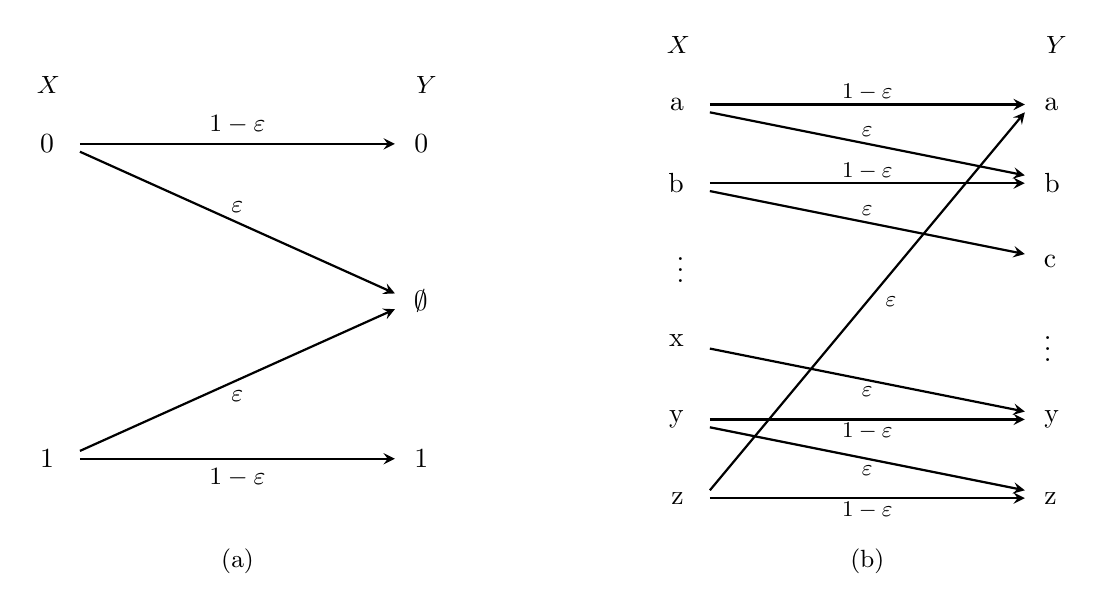
\begin{tikzpicture}
\shorthandoff{>}
%
% Canal borrador
\begin{scope}
\node at (-.4,2.75){\small $X$}; \node at (4.4,2.75){\small $Y$};
%
\draw[>=stealth,->,thick] (-.2,2) node[left]{0} (0,2) -- (4,2) node[right]{\ 0};
\node[above] at (2,2){\small $1-\varepsilon$};
%
\draw[>=stealth,->,thick] (-.2,-2) node[left]{1} (0,-2) -- (4,-2) node[right]{\ 1};
\node[below] at (2,-2){\small $1-\varepsilon$};
%
\draw[>=stealth,->,thick] (0,1.9)--(4,.1);
\node at (2,1.2){\small $\varepsilon$};
\draw[>=stealth,->,thick] (0,-1.9)--(4,-.1);
\node at (2,-1.2){\small $\varepsilon$};
\node[right] at (4,0){\ $\emptyset$};
%
\end{scope}
%
% Canal typewriter
\begin{scope}[xshift = 8cm]
\node at (-.4,3.25){\small $X$}; \node at (4.4,3.25){\small $Y$};
%
% lineas sin error
\draw[>=stealth,->,thick] (-.2,2.5) node[left]{a} (0,2.5) -- (4,2.5) node[right]{\ a};
\node[scale=.9] at (2,2.65){\small $1-\varepsilon$};
\draw[>=stealth,->,thick] (-.2,1.5) node[left]{b} (0,1.5) -- (4,1.5) node[right]{\ b};
\node[scale=.9] at (2,1.65){\small $1-\varepsilon$};
\node[left] at (-.2,.5){$\vdots$}; \node[right] at (4,-.5){\ $\vdots$};
\draw[>=stealth,->,thick] (-.2,-1.5) node[left]{y} (0,-1.5) -- (4,-1.5) node[right]{\ y};
\node[scale=.9] at (2,-1.65){\small $1-\varepsilon$};
\draw[>=stealth,->,thick] (-.2,-2.5) node[left]{z} (0,-2.5) -- (4,-2.5) node[right]{\ z};
\node[scale=.9] at (2,-2.65){\small $1-\varepsilon$};
%
% lineas con el error
\draw[>=stealth,->,thick] (0,2.4) -- (4,1.6);
\node[scale=.9] at (2,2.15){\small $\varepsilon$};
\draw[>=stealth,->,thick] (0,1.4) -- (4,.6); \draw (4,.5) node[right]{\ c};
\node[scale=.9] at (2,1.15){\small $\varepsilon$};
\draw[>=stealth,->,thick]  (-.2,-.5) node[left]{x} (0,-.6) -- (4,-1.4);
\node[scale=.9] at (2,-1.15){\small $\varepsilon$};
\draw[>=stealth,->,thick] (0,-1.6) -- (4,-2.4);
\node[scale=.9] at (2,-2.15){\small $\varepsilon$};
\draw[>=stealth,->,thick] (0,-2.4) -- (4,2.4);
\node[scale=.9] at (2.3,0){\small $\varepsilon$};
%
\end{scope}
\node at (2,-3.3){\small (a)};
\node at (10,-3.3){\small (b)};
\end{tikzpicture}
 \end{center}
%
\leyenda{Ejemplos de canales discretos usuales.  (a): canal borrador, donde un 0
  (de probabilidad de ocurrencia $r$) o 1 (de probabilidad de occurrencia $1-r$)
  puede  transmitirse correctamente or  ser borado/perdido  (estado $\emptyset$)
  con una  probabilidad $\varepsilon$.   Se calcula $I_2(X;Y)  = (1-\varepsilon)
  h_2(r)$, dando la capacidad $C_2  = 1-\varepsilon$, alcanzada para una entrada
  uniforme.   (b): canal tipo  machina de  escribir~\protect\footnotemark, donde
  cada letra  de un ensemble  de $n$  letras (ac\'a con  $n = 26$)  se transmite
  correctamente con una probabilidad $1-\varepsilon$  o a la letra siguiente (de
  manera c\'iclica) con una probabilidad $\varepsilon$.  De $I_n(X;Y) = H_n(Y) -
  H_n(Y|X) = H_n(Y)  - h_n(\varepsilon)$ se deduce que $I_n$  es m\'axima si $Y$
  es  uniforme,  lo que  es  posible  si  $X$ es  uniforma,  dando  $C_n =  1  -
  h_n(\varepsilon)$.}
\label{Fig:SZ:CanalesDiscretos}
\end{figure}
%
\footnotetext{Se mencionar\'a de  que en toda esta subsecci\'on,  no se necesita
  de que  $X$ y/o  $Y$ sean  variables aleatorias reales,  \ie pueden  tomar sus
  valores sobre cualquier espacio discreto (por ejemplo de letras).}


% ================================= canal gaussiano

\subseccion{Canal de transmisi\'on continuo gaussiano y su capacidad}
\label{Ssec:SZ:Canalgaussiano}

Un canal de  comunicaci\'on continuo relativamente simple es  conocido como {\it
  canal  gaussiano}~\cite[Sec.~25]{Sha48},~\cite{CovTho06,  Rio07}:  $X$ es  una
variable continua definida  sobre $\X \subset \Rset^d$ y la  salida $Y$ es una
versi\'on ruidosa de $X$, \ie $Y =  X + \xi$ con el ruido $\xi$ independiente de
$X$. En  el canal gaussiano, $\xi  \equiv \N$ es un  vector gaussiano.  Este
canal es tambi\'en definido por  su densidad de probabilidad ``de transici\'on''
$p_{Y|X=x}(y)$,  \ie por  la distribuci\'on  del ruido.   Tal canal  es descrito
figura  Fig.~\ref{Fig:SZ:CanalGaussiano}.   Se  supone  conocida  la  matriz  de
covarianza $\Sigma_\N$ del ruido, y se  nota $\Sigma_X$ la de la entrada. En
pr\'actica, no se puede mandar un mensaje a una potencia tan alta que se quiere,
lo que se traduce por una limitaci\'on
%
\[
\Tr\left(  \Sigma_X  \right) \le  \P,
\]
%
potencia l\'imite permitida por sampleo.

\begin{figure}[h!]
%
\begin{center} 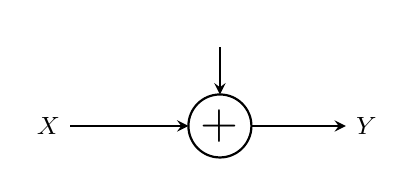
\begin{tikzpicture}
\shorthandoff{>}
%
%
% entrada
\draw[>=stealth,->,thick] (0,0) node[left]{\small $X$} --(1.5,0);
%
% adicion del ruido
\draw[thick] (1.9,0) circle (.4);
\draw[>=stealth,->,thick] (1.9,1) node[above]{\small $\Gauss$} --(1.9,.4);
\draw (1.9,0) node[align=center,scale=1.5]{\large +};
%
% salida
\draw[>=stealth,->,thick] (2.3,0)--(3.5,0) node[right]{\small $Y$};
\end{tikzpicture}
 \end{center}
%
\leyenda{Canal gaussiano. La entrada $X$, modelizada por un vector aleatorio, es
  corrupta aditivamente por un ruido gaussiano $\N$ independiente de $X$. La
  salida es entonces $Y = X + \N$ y el canal es completamente descrito por \
  $p_{Y|X=x}(y)   =   p_\N(y-x)$  \   (obviamente   independiente  de   la
  distribuci\'on de la entrada).}
%
\label{Fig:SZ:CanalGaussiano}
\end{figure}


Por  definici\'on, la informaci\'on  mutua $I(X;Y)$  entrada-salida es  dada por
$I(X;Y) = H(Y) - H(Y|X) = H(Y) - H(\N)$. Maximizar $I(X;Y)$ es equivalente a
maximizar  $H(Y) =  H(X  + \N)$  sujeto  a $\Tr\left(  \Sigma_X \right)  \le
\P$. Fijando  un $\Sigma_X$, la  propiedad~\ref{Prop:SZ:cotamaximagaussiana} \ de
la entrop\'ia diferencial implica que $H(Y)$  sea m\'axima si y solamente si $Y$
es gaussiana,  es decir  si y solamente  si $X$  est gaussiana, dando  $I(X;Y) =
\frac12  \log \left|  \Sigma_X +  \Sigma_\N  \right| -  \frac12 \log  \left|
  \Sigma_\N \right|$. Tomando en cuenta  el l\'imite de potencia, hace falta
maximizar $\left| \Sigma_X  + \Sigma_\N \right|$ sujeto a  $\Tr \Sigma_X \le
\P$ \  y \ $\Sigma_X  \ge 0$ sim\'etica  lo que no  es trivial.  Se  encuentra el
enfoque  permitiendo solucionar  el problema  en~\cite[Sec.~9.4]{CovTho06}.  Sea
$U$, matriz  ortogonal ($U U^t =  U^t U = I$)  de los autovectores  de la matriz
$\Sigma_\N  \ge 0$  sim\'etica~\footnote{Se  recordar\'a de  que  $A \ge  0$
  significa que $A$  es definida no negativa.}, de  columnas $u_i$ ordenadas tal
que los autovalores corespondientes  $\lambda^\N_i$ sean en orden creciente,
\ie
%
\[
\Sigma_\N  =  U  \Diag\left(  \begin{bmatrix} \lambda^\N_1  &  \cdots  &
    \lambda^\N_d \end{bmatrix}^t \right) U^t  \qquad \mbox{con} \qquad 0 \le
\lambda^\N_1 \le \cdots \le \lambda^\N_d,
\]
%
donde $\Diag$ es la matriz diagonal teniendo los $\lambda_i$ en su diagonal (ver
notaciones).   Sea \ $R_X  = U^t  \Sigma_X U$.   Es sencillo  ver que  \ $\left|
  \Sigma_X + \Sigma_\N \right| = \left| R_X + \Lambda_\N \right|$ \ (de $|A B| =
|A| \,  |B|$) \ y  que \ $\Tr \Sigma_X  = \Tr R_X$  (de $\Tr(A B) =  \Tr(B A)$).
Entonces, el problema se reduce a  maximizar \ $\left| R_X + \Lambda_\N \right|$
\ sujeto a \  $\Tr R_X \le \P$ \ y \ $R_X \ge  0$ sim\'etica.  La desigualdad de
Hadamard ya evocada da \ $\left| R_X + \Lambda_\N \right| \le \prod_i \left( R_X
  +  \Lambda_\N  \right)_{i,i}  =  \prod_i  \left( \left(  R_X  \right)_{i,i}  +
  \lambda^\N_i   \right)$   \  donde   $(\cdot)_{i,i}$   denota  el   componente
$(i,i)$-\'esima  de la  matriz, con  igualdad si  y solamente  si \  $R_X$  \ es
diagonal: para maximizar \ $\left| R_X + \Lambda_\N \right|$, \ $R_X$ \ debe ser
entonces  diagonal (dada  una  diagonal, se  alcanza  el m\'aximo  si los  otros
t\'erminos son  nulos).  Es decir  que la base  que diagonaliza \  $\Sigma_\N$ \
debe  diagonalizar  tambi\'en $\Sigma_X$.   Sean  ahora  \  $\lambda^X_i$ \  los
t\'erminos  diagonales   de  $R_X$:  queda  que  maximizar   \  $\prod_i  \left(
  \lambda^X_i + \lambda^\N_i \right)$ \ sujeto a $\sum_i \lambda^X_i \le \P$ \ y
\ $\lambda^X_i \ge 0$.  Este problema de optimizaci\'on sujeto a una desigualdad
se  resuelva  con el  enfoque  de  Karush-Kuhn-Tucker~\footnote{Se introduce  el
  factor de Lagrange y se  maximiza \ $\prod_i \left( \lambda^X_i + \lambda^\N_i
  \right) +  \eta \sum_i \lambda^X_i$.  Eso  da \ $\lambda^X_i  + \lambda^\N_i =
  \lambda$ \  constante si $\lambda$ es  tal que se satisfaga  la positividad de
  $\lambda^X_i$, y $\lambda^X_i = 0$  sino.  En otras palabras, \ $\lambda^X_i =
  \left( \lambda -  \lambda^\N_i \right)_+$ con $\lambda$ el  factor de Lagrande
  despu\'es  de una  reescritura.  Queda  que maximizar  los  $\lambda^X_i$ para
  maximizar $\left| R_X + \Lambda_\N \right|$, es decir tomar $\lambda$ lo m\'as
  grande  que se  puede, pero  satisfaciendo  $\sum_i \lambda^X_i  \le \P$,  \ie
  alcanzando  la   igualdad.\label{Foot:SZ:KKT}}  (KKT)~\cite{Mil00,  CamMar09},
dando  \  $\lambda^X_i  = \left(  \lambda  -  \lambda^\N_i  \right)_+$ \  con  \
$(\cdot)_+ = \max(\cdot,0)$ \ y \ $\lambda$ \ tal que \ $\sum_i \left( \lambda -
  \lambda^\N_i \right)_+ = \P$.  En conclusi\'on, la capacidad es dada por
%
\begin{eqnarray*}
C =  \frac12 \log \left(  \frac{\left| \Sigma_\N +  \Sigma_X \right|}{\left|
      \Sigma_\N  \right|}  \right)  & \quad \mbox{con} \quad &  \Sigma_X  =  U
\Diag\left( \begin{bmatrix} \left(\lambda - \lambda^\N_1\right)_+ & \cdots & \left(\lambda -
    \lambda^\N_d \right)_+ \end{bmatrix}^t \right) U^t,\\[2.5mm]
%
& &  \lambda \ \mbox{ tal que } \:
\sum_i \left(\lambda - \lambda^\N_i \right)_+ = \P
\end{eqnarray*}
%
alcanzada por $X$ gaussiano de matriz de covarianza $\Sigma_X$ as\'i construida.

La  \'ultima condici\'on  se resuelva  a  trav\'es de  lo que  es conocido  como
``llenado   de   agua''   (water-filling   en   ingl\'es),   illustrado   figura
Fig.~\ref{Fig:SZ:WaterFilling}.   El  principio  es  parecido  a  tener  niveles
$\lambda^\N_i$  representando  las  potencias  del  ruido (en  la  base  que
diagonaliza la  matriz de covarianza), y  de ``llenar con agua''  hasta un nivel
$\lambda$ tal que el ``volumen''  a\~nadido vale $\P$; en cada $\lambda^\N_i$
se ha a\~nadido el $\lambda^X_i$~\cite[Sec.~9.4]{CovTho06}.

\begin{figure}[h!]
%
\begin{center} \begin{tikzpicture}
\shorthandoff{>}
%
% Filling
\filldraw[fill=gray!30] (3,2)--(3,1.5)--(2,1.5)--(2,1)--(1,1)--(1,.75)--(0,.75)--(0,2);
%
%Axes
\draw[>=stealth,->] (-.1,0)--(6,0);% node[right]{\small $i$};
\draw[>=stealth,->] (0,-.1)--(0,3);
\node[left] at (0,.85){\rotatebox{90}{\footnotesize Potencias}};
%
% neveles de ruido
\draw[thick] (0,.75)--(1,.75)--(1,0);             \node at (.5,.375){\small $\lambda^\N_1$};
\draw[thick] (1,.75)--(1,1)--(2,1)--(2,0);        \node at (1.5,.5){\small $\lambda^\N_2$};
\draw[thick] (2,1)--(2,1.5)--(3,1.5)--(3,0);      \node at (2.5,.75){\small $\lambda^\N_3$};
\draw[thick] (3,1.5)--(3,2.25)--(4,2.25)--(4,0);  \node at (3.5,1.125){\small $\lambda^\N_4$};
\draw[thick] (4,2.25)--(4,2.75)--(5,2.75)--(5,0); \node at (4.5,1.375){\small $\lambda^\N_5$};
\draw[thick] (5.5,1.25) node{\bf $\cdots$};
%
% nivel lambda y potencias de los X
\draw[thick] (0,2) node[left]{\small $\lambda$}--(3,2);
\draw (1,.75)--(1,2); \node at (.5,1.375){\small $\lambda^X_1$};
\draw (2,1)--(2,2);   \node at (1.5,1.5){\small $\lambda^X_2$};
\draw (3,1.5)--(3,2); \node at (2.5,1.75){\small $\lambda^X_3$};
\end{tikzpicture}
 \end{center}
%
\leyenda{Principio   del  ``water-filling''   para  obtener   los  $\lambda^X_i$
  satisfaciendo  el v\'inculo de  potencia l\'imite  y permitiendo  de construir
  $\Sigma_X$ a partir  de la matriz diagonal de los $\lambda^X_i$  y la base que
  diagonaliza  la  covarianza  $\Sigma_\N$  del  ruido.  La  zona  en  grise
  representa esquem\'aticamente $\P$.}
%
\label{Fig:SZ:WaterFilling}
\end{figure}

En   el   caso   escalar,   se   obtiene
%
\[
C = \frac12 \log\left( 1 + \frac{\P}{\sigma_\N^2} \right),
\]
%
donde     $\frac{\P}{\sigma_\N^2}$     es     conocido    como     relaci\'on
se\~nale-ruido~\footnote{Esta formula es muy  parecida a la de Shannon, Laplume,
  o Clavier~\cite{Sha48,  Lap48, Cla48} (ver tambi\'en~\cite[Sec.~9.3]{CovTho06}
  o~\cite[Sec.~11.2]{Rio07}).   De hecho,  si se  considera  s\'imbolos mandados
  durante  $T$ segundos  cada  uno (s\'imbolos  puestos  en forma  para dar  una
  se\~nal anal\'ogica) usando una banda  de transmisi\'on $B$, por el teorema de
  Nyquist $B = \frac{1}{2 T}$ (caso l\'imite). Si el ruido es blanco en la banda
  $B$, de densidad espectral de potencia por unidad de frecuencia igual a $N_0$,
  para  un  s\'imbolo  la  relaci\'on  se\~nal-ruido  se  escribe  $\frac{\P}{N_0
    B}$. Adem\'as,  se calcula en general  la capacidad por unidad  de tiempo es
  decir la capacidad  por s\'imbolo divido por  $T = \frac{1}{2 B}$, \ie  $C = B
  \log\left( 1 +  \frac{\P}{N_0 B} \right)$ por segundos,  lo que es precisamente
  la capacidad calculdada por Shannon.  Esta es a veces conocida como formula de
  Shannon-Hartley.}

En~\cite{CovTho06,  Rio07}  por ejemplo,  se  dan  otros  ejemplos de  canal  de
comunicaci\'on   en   el   contexto   continuo   (entrada   $X_t$   siendo   una
se\~nal/proceso, canal filtrando, canal con retroacci\'on (o feedback), etc.).

% ================================= codificacion

\subseccion{Codificaci\'on entr\'opica sin perdida}
\label{Ssec:SZ:Codificacion}

El  problema  de  codificaci\'on  de  fuente  puede  presentarse  de  la  manera
siguiente~\cite[cap.~5]{CovTho06}  o   \cite[cap.~13]{Rio07}.   Sea  un  proceso
aleatorio $\left\{  X_t \right\}_{t \in \Zset}$,  supuesto estacionario, llamado
{\it  fuente}, donde  los $X_t$  toman sus  valores sobre  un  alfabeto discreto
finito no necesariamente real ($X$ puede tomar cualquier etiqueta)
%
\[
\X = \{ x_1 \, , \, \ldots \, , \, x_\alpha \} \qquad \mbox{alfabeto fuente},
\]
%
de  distribuci\'on  $p_X$.   A  cada posible  secuencia~\footnote{Por  abuso  de
  escritura una  cadena de  $n$ s\'imbolos puede  ser vista como  un $n$-uplet.}
$s_1  \cdots s_n \in  \X^n$ de  letras de  $\X$, se  quiere asignar  un c\'odigo
$c(s_1 \cdots s_n)$ de letras de un alfabeto discreto finito,
%
\[
\C = \{ \cod_1 \, , \, \ldots \, , \, \cod_d \} \qquad \mbox{ alfabeto c\'odigo}.
\]
%
El c\'odigo es dicho {\it $d$-ario}.   Por ejemplo, se puede asignar un c\'odigo
$c(x_i)  = \cod_{i,1}  \cdots  \cod_{i,l_i} \in  \C^{l_i}$  a cada  s\'imbolo $x_i$,
c\'odigo llamado  {\it palabras c\'odigos}, y  a secuencias $s_1  \cdots s_n$ la
concatenaci\'on de las palabras  c\'odigos correspondiente a cada s\'imbolo, \ie
el  c\'odigo $c(s_1) \cdots  c(s_n)$.  En  el sistema  Moorse por  ejemplo, $\C$
consiste en  un punto,  una barra,  una espacio entre  letras, un  espacio entre
palabras.  En una computadora en general todo  se codifica en bits $\C = \{ 0 \,
, \, 1\}$.  M\'as formalmente, sean
%
\[
\F_\X   =   \bigcup_{k=0}^{\infty}  \X^k   \qquad   \mbox{y}   \qquad  \F_\C   =
\bigcup_{k=0}^{\infty} \C^k,
\]
%
uni\'on  de  secuencias de  $k$  letras de  $\X$  y  $\C$ respectivamente.   Una
codificaci\'on de  fuente consiste  en una  funci\'on de \  $\F_\X$ \  dentro de
$\F_\C$. En lo  que sigue, nos concentramos en  c\'odigos definidos para bloques
de s\'imbolos de tama\~no $m \ge 1$:
%
\[
\begin{array}{lccl}
c_m: & \X^m & \rightarrow & F_\C\\[.5mm]
%
& x & \mapsto & c_m(x) \in \C^{l_{c_m}(x)}
\end{array},
\]
%
donde $l_{c_m}(x) \in \Nset^*$ es el  {\it largo} de la palabra c\'odigo $c_m(x)$,
y
%
\[
\forall \,  n \ge 1,  \quad \forall  \, s_1 \cdots  s_n \in \big(  \X^m \big)^n,
\quad c_m(s_1 \cdots s_n) \equiv c_m(s_1) \cdots c_m(s_n),
\]
%
lo  que  es  llamado {\it  extensi\'on  del  c\'odigo}.   En  lo que  sigue,  se
escribir\'a $c \equiv c_1$.

Una manera ingenua de codificar consiste a apoyarse sobre la descomposici\'on de
base \ $d$  \ de un entero, \ie para  $1 \le i \le \alpha$  se puede escribir de
manera \'unica \ $i-1 = (i_0-1) + (i_1-1) d + \cdots + (i_K-1) d^K$ \ donde \ $K
= \Big\lceil \log_d |\X| \Big\rceil$ \ y \ $1 \le i_k \le \alpha$.  Entonces, se
puede asignar la palabra c\'odigo \ $c(x_i) = \cod_{i_0} \cdots \cod_{i_k}$ \ al
s\'imbolo  $x_i$.  Haciendo  eso, cada  palabra c\'odigo  tieno el  mismo largo.
Pero, es m\'as  econ\'omico hacer una codificaci\'on dicha  de largos variables,
teniendo   en  cuenta  las   probabilidades  de   aparici\'on  de   cada  $x_i$.
Implicitamente, es la idea del c\'odigo  de Moorse, que asigna un punto o series
de puntos o  c\'odigo peque\~no a las letras muy frecuentes  (ej.  un punto para
el `e',  dos puntos para el  `i', etc.), y  barras o combinaciones largas  a las
letras que son raras (ej. bara-bara-punto-bara para el `q' o cinco baras para el
`0').  Dicho de  otra manera, el c\'odigo ingenuo  ser\'ia ``eficaz'' para $x_i$
apareciendo con las mismas frecuencias/probabilidades.

En los c\'odigos de largos variables (incluyendo el c\'odigo ingenuo), volviendo
a  $c_m$, existen  varios tipos  de  c\'odigos.  Un  c\'odigo es  dicho {\it  no
  singular} si $c_m$  es inyectiva: a cada $x \in  \X^m$ corresponde una palabra
c\'odigo \'unica. Esta propiedad es un requisito que parece obvio querer para un
c\'odigo.  Pero  no es suficiente  para poder decodificar un  mensaje, compuesta
por una  secuencia de palabras  c\'odigo.  Lo importante  en este caso  es poder
decodificar  la   secuencia  sin  ambig\"uedad:  un  c\'odigo   est  dicho  {\it
  descifrable} o {\it  a decodificaci\'on \'unica} (o sin  perdida) si todas las
extensiones son no singulares.
%
\begin{ejemplo}[C\'odigo no singular, pero no decifrable]
\label{Ej:SZ:CodigoNoSingularDecifrable}
%
Sean \ $\X = \{ \aleph \, , \, \beth \, , \, \gimel \, , \, \daleth \}$, \ $\C =
\{0 \, , \, 1  \}$ \ y \ $c(\aleph) = 0, \: c(\beth) =  00, \: c(\gimel) = 1, \:
c(\daleth) =  01$ ($m = 1$).  El  c\'odigo es no singular,  pero no descifrable.
La  secuencia  $0010$  puede  provenir  de $\aleph\aleph\gimel\aleph$,  \  de  \
$\aleph\daleth\aleph$ \ o de \ $\beth\gimel\aleph$.
\end{ejemplo}
%
Obviamente,  se  requiere  en  general  de  un  c\'odigo  que  sea  descifrable.
Frecuentemente,  se requiere tambi\'en  poder decodificar  sobre la  marcha, sin
esperar de medir toda la secuencia  codificada: es lo que se llama {\it c\'odigo
  instantaneo}.
%
\begin{ejemplo}[C\'odigo decifrable, pero no instantaneo]
\label{Ej:SZ:CodigoDcifrableNoInstantaneo}
%
  Sea el  c\'odigo $c(\aleph)  = 00,  \: c(\beth) =  10, \:  c(\gimel) =  11, \:
  c(\daleth)  =  110$.  Este  c\'odigo  es  descifrable,  pero  no  instantaneo.
  Considera la secuencia  $0011011$ y marcha sobre ella.  $0$  no es una palabra
  c\'odigo; $00$  es y sin  ambig\"uedad proviene de  un $\aleph$ (no  hay otras
  palabras  empezando por $00$);  luego $1$  no es  una palabra,  y $11$  es una
  palabra  c\'odigo,  pero se  necesita  adelantar para  saber  si  viene de  un
  $\gimel$ o de un $\daleth$; la  letra siguiente siendo un $0$, todav\'ia no se
  puede concluir si $110$ vino de  $\gimel$ y alg\'o o $\daleth$.  Al final, con
  $1101$, se  sabe que se tuvimos  un $\daleth$ porque  ninguna palabra c\'odigo
  empieza por $01$.   Al final, sin ambig\"uedad el  antecedente de la secuencia
  binaria era  $\aleph\daleth\gimel$.  Pero se necesit\'o marchar  sobre toda la
  secuencia antes de decodificar.
\end{ejemplo}
%
Obviamente,  un c\'odigo  instantaneo es  tal  que ninguna  palabra c\'odigo  es
prefijo de una otra, \ie si $c_m(x)$ es una palabra c\'odigo, las otras palabras
c\'odigo no  pueden empezar  con $c_m(x)$; el  c\'odigo es tambi\'en  dicho {\it
  libre  de  prefijo}.   Estas   distinciones  estan  ilustradas  en  la  figura
Fig.~\ref{Fig:SZ:ClasesCodigos} (ver~\cite[cap.~5]{CovTho06}).

\begin{figure}[h!]
%
\begin{center} 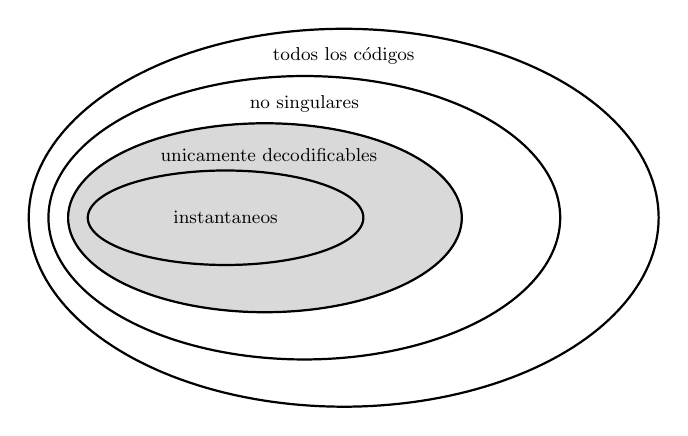
\begin{tikzpicture}
\shorthandoff{>}
\filldraw[fill=gray!30,domain=0:360, samples=200] plot ({2.5*cos(\x)+.5},{1.2*sin(\x)});
%%%%
\draw[thick,domain=0:360, samples=200] plot ({1.75*cos(\x)},{.6*sin(\x)});
\node[scale=.75] at (0,0){\small instantaneos};
%
\draw[thick,domain=0:360, samples=200] plot ({2.5*cos(\x)+.5},{1.2*sin(\x)});
\node[scale=.75] at (.55,.8){\small  unicamente decodificables};
%
\draw[thick,domain=0:360, samples=200] plot ({3.25*cos(\x)+1},{1.8*sin(\x)});
\node[scale=.75] at (1,1.45){\small no singulares};
%
\draw[thick,domain=0:360, samples=200] plot ({4*cos(\x)+1.5},{2.4*sin(\x)});
\node[scale=.75] at (1.5,2.05){\small todos los c\'odigos};
\end{tikzpicture}
 \end{center}
%
\leyenda{Clases  de c\'odigos.   Los  c\'odigos  contienen la  clase  de los  no
  singulares.  La misma  contiene la clase de los  c\'odigos descifrables.  Ella
  contiene los  c\'odigos instantaneos.  En  grise se representan las  clases de
  c\'odigos sin perdida a lo cuales se dedica esta secci\'on.}
%
\label{Fig:SZ:ClasesCodigos}
\end{figure}

Adem\'as  de   la  decodificaci\'on  sin   ambig\"uedad,  una  caracterizaci\'on
importante del  c\'odigo es la  taza de codificaci\'on~\footnote{En~\cite{Rio07}
  por  ejemplo, se  define esta  taza suponiendo  que cada  secuencia  fuente es
  codificada por el  mismo n\'umero de bits. La taza es  entonces el n\'umero de
  bits por s\'imbolo.}
%
\[
R_{c_m} = \frac{\log_d \left( \sum_{x \in \X^m} l(x) P(X = x) \right)}{m},
\]
%
donde $X$  representa una  secuencia de $m$  variables $X_t$.  El  argumento del
logaritmo (de base adecuada al cardenal  de $\C$) es el {\it largo promedio} del
c\'odigo. Por ejemplo,  para $d = 2$, $R_{c_m}$ es el  n\'umero de bits promedio
del c\'odigo por s\'imbolo.

En general,  se quiere minimizar $R_{c_m}$  (compresar el mensaje  a mandar), lo
que puede  ser contradictorio con la  necesidad de a\~nadir  redundancia para no
perder  informaci\'on   durante  una  transmisi\'on.   En  lo   que  sigue,  nos
concentramos en  el problema  de compresi\'on,  sin tener en  cuenta el  paso de
transmisi\'on  de  mensajes codificados  en  un  canal.   Minimizar la  taza  es
equivalente a minimizar el largo  promedio. Adem\'as, se puede focalisarse en $m
= 1$; todo se extiende sencillamente a $m > 1$.

La meta de  la compresi\'on es entonces construir  un c\'odigo $c$, descifrable,
que minimizar el largo promedio
%
\[
L(c) = \sum_{x \in \X} p_X(x) \, l(x).
\]
%
Antes de ir  m\'as adelante, hace falta traducir en  ecuaci\'on el v\'inculo que
$c$    sea    descifrable.    Eso    es    dado    por    la   desigualdad    de
Kraft-McMillan~~\cite{Kra49,   McM56,   Kar61}~\footnote{Esta  desigualdad   fue
  probabada  por  L.  G.   Kraft  para c\'odigos  instantaneos  en  su tesis  de
  maestria~\cite{Kra49}.  Luego, fue extendida  a los c\'odigos descifrables por
  B.  McMillan~\cite{McM56} (en  una nota de pie de pagina  de su papel, atribua
  esta  observaci\'on a J.   L.  Doob  hecha oralemente  durante una  escuela de
  verano en Ann Arbor, MI en agosto 1955).}
%
\begin{teorema}[Desigualdad de Kraft-McMillan]
\label{Teo:SZ:KraftMcMillan}
%
  Los largos  $l_c(x)$ de las palabras  c\'odigo de un  c\'odigo $c$ descifrable
  deben satisfacer la desigualdad
  %
  \[
  \sum_{x \in \X} d^{-l_c(x)} \le 1.
  \]
  %
  Rec\'iprocamente,  para cada  conjunto de  enteros $\{  \ell_x \}_{x  \in \X}$
  satisfaciendo  esta   desigualdad,  es   posible  de  construir   un  c\'odigo
  descifrable con $l_c(x) = \ell_x$.
\end{teorema}
%
\begin{proof}
  Para cualquier $k \ge 1$ y cualquiera  cadena $s = s_1 \cdots s_k \in \X^k$, la
  extensi\'on  del  c\'odigo,  $c_k(s_1  \cdots  s_k) =  c(s_1)  \cdots  c(s_k)$
  satisface $l_{c_k}(s) = \sum_{i=1}^k l_c(s_i)$. Entonces
  %
  \[
  \left(  \sum_{x  \in \X}  d^{-l_c(x)}  \right)^k \:  =  \:  \sum_{\bar{x} \in  \X^k}
  d^{-l_{c_k}(\bar{x})} \: = \: \sum_{m=1}^{k \, l_c^{\max}} \#(m) \, d^{-m},
  \]
  %
  re-escribiendo  la segunda  suma, agrupando  los t\'erminos  de  mismo largos,
  donde $\#(m)$  es el n\'umero de c\'odicos  de $\X^k$ teniendo el  largo $m$ y
  $l_c^{\max}  =  \max_{x  \in  \X}  l_c(x)$  es el  largo  mayor.   $c$  siendo
  descifrable,  $c_k$ debe  ser inyectiva,  imponiendo $\#(m)  \le d^m$  (no hay
  m\'as palabras de  largo $m$ que el cardenal  de $\C^m$), dando inmediatemente
  que necesariamente
  %
  \[
  \forall \,  k \in \Nset^*, \quad \sum_{x  \in \X} d^{-l_c(x)} \le  \left( k \,
    l_c^{\max}  \right)^{\frac1k} \quad  \Leftrightarrow \quad  \sum_{x  \in \X}
  d^{-l_c(x)} \le \min_{k \in \Nset^*} \left( k \, l_c^{\max} \right)^{\frac1k}.
  \]
  %
  Un estudio r\'apido de \  $u \mapsto \left( u \, l_c^{\max} \right)^{\frac1u}$
  \ para \  $u \ge 1$ \ y  teniendo en cuenta de que $l_c^{\max}  \le 1$ permite
  concluir  que el  m\'inimo  es igual  a  1, terminando  la  parte directa  del
  teorema.

  Rec\'iprocamente, sea  \ $\{ \ell_x  \}_{x \in \X}$  \ un conjunto  de enteros
  satisfaciendo la  desigualdad de Kraft-McMillan.  Se puede  agrupar los largos
  iguales y  clasificarlos. Sea \ $n_\ell$ \  los n\'umeros de largos  igual a \
  $\ell =  1 , \ldots  , \ell^{\max} \le  \alpha$.  Consideramos ahora  un arbol
  empezando con una ra\'iz, correspondiente a un largo $0$, que se divide en $d$
  ramas, correspondiente a los largos iguales  a $1$; a cada nudo se asocian las
  letras \  $\cod_1, \ldots , \cod_d$. Esto  nudos se dividen cada  uno en $d$
  otras  ramas, y  los nudos  de ``padre''  \ $\cod_i$  \ se  va a  asociar las
  palabras c\'odigos \ $\cod_i \cod_1 , \ldots , \cod_i \cod_\alpha$, \ etc.
  Este  arbol,  conocido  como  arbol  de  Kraft,  es  ilustrado  en  la  figura
  Fig.~\ref{Fig:SZ:ArbolKraft}  para \  $d =  2$  \ y  \ $\C  =  \{0 \,  , \,  1
  \}$. Claramente, \ $n_1 \le d$ \ si no \ $n_1 \, d^{-1} > 1$ \ y los largos no
  podr\'ian  satisfacer  la  desigualdad  de Kraft-McMillan.   El  principio  es
  entonce de asociar a los \ $n_1$ \ (posiblemente igual a 0) largos iguales a \
  $1$ \ unos nudos con las palabras c\'odigo asociadas de largo \ $1$ \ (primera
  profundez  de  ramas)  y de  prohibir  todos  las  ramas  de padre  los  nudos
  seleccionados        (lineas        punteadas        en       la        figura
  Fig.~\ref{Fig:SZ:ArbolKraft}). Estos  nudos son  llamados {\em hojas}  (no hay
  ramas).  En  la capa de ``hijos'' de  profundez/largos \ $2$, quedan  \ $d^2 -
  n_1 \, d$ \ nudos (accessibles)  que se pueden dividir en ramas.  Nuevamente, \
  $n_2 \le d^2 - n_1 \, d$ \  sino tendr\'iamos \ $n_1 \, d^{-1} + n_2 \, d^{-2}
  > 1$, \ incompatible con la  desigualdad de Kraft-McMillan. Se puede asociar a
  los \ $n_2$  \ largos iguales a \  $2$ \ unos nudos con  las palabras c\'odigo
  asociadas de  largo \ $2$  \ (segunda profundez),  y de prohibir que  salen de
  estos nudos  nuevas ramas (son entonces  hojas en la  segunda profundez), etc.
  Haciendo as\'i, se asocia un c\'odigo \  $c$ \ de largos \ $l_c(x) = \ell_x$ \
  que aparece libre  de prefijo, es decir instantaneo.   Entonces, este c\'odigo
  es tambi\'en descifrable.
\end{proof}

A este punto, se menciona los hechos siguientes
%
\begin{itemize}
\item  Los  largos de  un  c\'odigo  descifrable  satisfacen la  desigualdad  de
  Kraft-McMillan,  pero con  el  conjunto de  largos  correspondientes se  puede
  siempre  construir un c\'odigo  instantaneo.  Claramente,  se puede  buscar un
  c\'odigo de largo promedio m\'inimo  en los c\'odigos instantaneo, sin perdida
  de optimalidad (buscar en la clase  m\'as amplia de los descifrable no permite
  bajar el largo promedio).
%
\item En  los c\'odigos  libres de prefijo,  si se  fija el n\'umero  de hojas
  (\'ultima   profundez)  borradas   contruyendo  un   c\'odigo,  este   vale  \
  $\sum_{i=1}^{\ell^{\max}}  n_i  \,  d^{\ell^{\max}  -  i} =  \sum_{x  \in  \X}
  d^{\ell^{\max} -  l_c(x)}$.  \ Es  necesariamente menor que el  n\'umero total
  $d^{\ell^{\max}}$  de hojas,  lo  que  prueba el  teorema  para los  c\'odigos
  instantaneos~\cite{Kra49, Kar61}.
%
\item El teorema  se generaliza obviamente para codificar  una fuente (discreta)
  con un n\'umero infinito de estados, tomando el l\'imite $\alpha \to \infty$.
%
\item Si se conocen los largos  \'optimos, es suficiente para poder construir un
  c\'odigo libre de prefijo.
\end{itemize}

\begin{figure}[h!]
%
\begin{center} 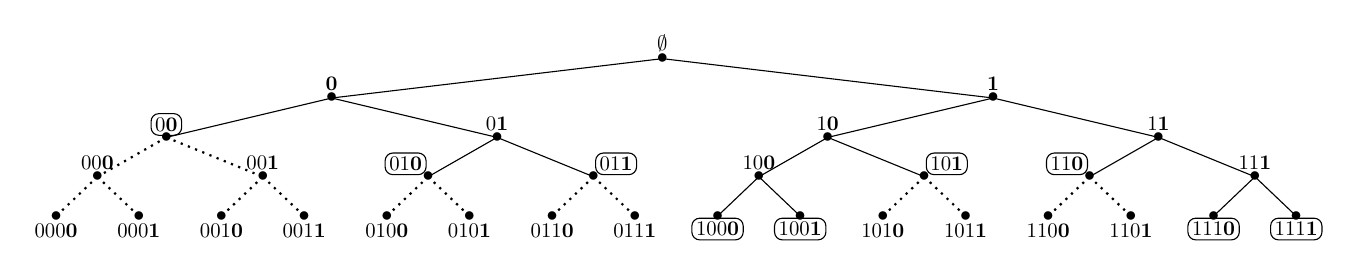
\begin{tikzpicture}[xscale=1.4]
\shorthandoff{>}
%
% nivel 2^4
%%%%%%%%%%%%
\draw[thick,dotted] (.375,.5)--(0,0) node[scale=.8]{$\bullet$} node[below,scale=.75]{000\textbf{0}};
\draw[thick,dotted] (.375,.5)--(.75,0) node[scale=.8]{$\bullet$} node[below,scale=.75]{000\textbf{1}};
\draw[thick,dotted] (1.875,.5)--(1.5,0) node[scale=.8]{$\bullet$} node[below,scale=.75]{001\textbf{0}};
\draw[thick,dotted] (1.875,.5)--(2.25,0) node[scale=.8]{$\bullet$} node[below,scale=.75]{001\textbf{1}};
\draw[thick,dotted] (3.375,.5)--(3,0) node[scale=.8]{$\bullet$} node[below,scale=.75]{010\textbf{0}};
\draw[thick,dotted] (3.375,.5)--(3.75,0) node[scale=.8]{$\bullet$} node[below,scale=.75]{010\textbf{1}};
\draw[thick,dotted] (4.875,.5)--(4.5,0) node[scale=.8]{$\bullet$} node[below,scale=.75]{011\textbf{0}};
\draw[thick,dotted] (4.875,.5)--(5.25,0) node[scale=.8]{$\bullet$} node[below,scale=.75]{011\textbf{1}};
%
\draw (6.375,.5)--(6,0) node[scale=.8]{$\bullet$}
node[inner sep=2pt,outer sep=1pt,draw=black,below,scale=.75,rounded corners=1mm]{100\textbf{0}};
%
\draw (6.375,.5)--(6.75,0) node[scale=.8]{$\bullet$}
node[inner sep=2pt,outer sep=1pt,draw=black,below,scale=.75,rounded corners=1mm]{100\textbf{1}};
%
\draw[thick,dotted] (7.875,.5)--(7.5,0) node[scale=.8]{$\bullet$} node[below,scale=.75]{101\textbf{0}};
\draw[thick,dotted] (7.875,.5)--(8.25,0) node[scale=.8]{$\bullet$} node[below,scale=.75]{101\textbf{1}};
\draw[thick,dotted] (9.375,.5)--(9,0) node[scale=.8]{$\bullet$} node[below,scale=.75]{110\textbf{0}};
\draw[thick,dotted] (9.375,.5)--(9.75,0) node[scale=.8]{$\bullet$} node[below,scale=.75]{110\textbf{1}};
%
\draw (10.875,.5)--(10.5,0) node[scale=.8]{$\bullet$}
node[inner sep=2pt,outer sep=1pt,draw=black,below,scale=.75,rounded corners=1mm]{111\textbf{0}};
%
\draw (10.875,.5)--(11.25,0) node[scale=.8]{$\bullet$}
node[inner sep=2pt,outer sep=1pt,draw=black,below,scale=.75,rounded corners=1mm]{111\textbf{1}};
%
%----------
%
% nivel 2^3
%%%%%%%%%%%%
\draw[thick,dotted] (1,1)--(.375,.5) node[scale=.8]{$\bullet$} node[above,scale=.75]{00\textbf{0}};
\draw[thick,dotted] (1,1)--(1.875,.5) node[scale=.8]{$\bullet$} node[above,scale=.75]{00\textbf{1}};
%
\draw (4,1)--(3.375,.5) node[scale=.8]{$\bullet$}
node[inner sep=2pt,outer sep=1pt,draw=black,above left,scale=.75,rounded corners=1mm]{01\textbf{0}};
%
\draw (4,1)--(4.875,.5) node[scale=.8]{$\bullet$}
node[inner sep=2pt,outer sep=1pt,draw=black,above right,scale=.75,rounded corners=1mm]{01\textbf{1}};
%
\draw (7,1)--(6.375,.5) node[scale=.8]{$\bullet$} node[above,scale=.75]{10\textbf{0}};
%
\draw (7,1)--(7.875,.5) node[scale=.8]{$\bullet$}
node[inner sep=2pt,outer sep=1pt,draw=black,above right,scale=.75,rounded corners=1mm]{10\textbf{1}};
%
\draw (10,1)--(9.375,.5) node[scale=.8]{$\bullet$}
node[inner sep=2pt,outer sep=1pt,draw=black,above left,scale=.75,rounded corners=1mm]{11\textbf{0}};
%
\draw (10,1)--(10.875,.5) node[scale=.8]{$\bullet$} node[above,scale=.75]{11\textbf{1}};
%
%----------
%
% nivel 2^2
%%%%%%%%%%%%
\draw (2.5,1.5)--(1,1) node[scale=.8]{$\bullet$}
node[inner sep=2pt,outer sep=1pt,draw=black,above,scale=.75,rounded corners=1mm]{0\textbf{0}};
%
\draw (2.5,1.5)--(4,1) node[scale=.8]{$\bullet$} node[above,scale=.75]{0\textbf{1}};
\draw (8.5,1.5)--(7,1) node[scale=.8]{$\bullet$} node[above,scale=.75]{1\textbf{0}};
\draw (8.5,1.5)--(10,1) node[scale=.8]{$\bullet$} node[above,scale=.75]{1\textbf{1}};
%
%----------
%
% nivel 2^1
%%%%%%%%%%%%
\draw (5.5,2)--(2.5,1.5) node[scale=.8]{$\bullet$} node[above,scale=.75]{\textbf{0}};
\draw (5.5,2)--(8.5,1.5) node[scale=.8]{$\bullet$} node[above,scale=.75]{\textbf{1}};
%
%----------
%
% nivel 2^0
%%%%%%%%%%%%
\draw (5.5,2) node[scale=.8]{$\bullet$} node[above,scale=.75]{$\emptyset$};

\end{tikzpicture} \end{center}
%
\leyenda{Arbol de  Kraft en el  caso binario ($d  = 2$). La ra\'iz,  de c\'odigo
  $\emptyset$ de largo 0, se divide en dos ramas, de c\'odigos respectivamente \
  $0$ \ y  \ $1$ \ (profundez \  $1$). Cada nudo de esta profundez  se divide en
  dos ramas (profundez dos), dando cuatros nuevos nudos con los c\'odigos \ $00$
  \ y $01$ de padre \ $0$, y \ $10$ \ y $11$ de padre \ $1$.  Etc.  En cada nudo
  de esta figura,  en el c\'odigo, se marca en  negrita la letra correspondiente
  al bit a\~nadido al c\'odigo padre.   Para hacer un c\'odigo libre de prefijo,
  una vez que un nudo es  seleccionado para ser una palabra c\'odigo (encuadrado
  en la  figura), no  puede tener nudos  ``hijos'' siendo tambi\'en  una palabra
  c\'odigo:  se boran  las ramas  saliendo  de un  nudo-palabra c\'odigo  (ramas
  punteadas).}
%
\label{Fig:SZ:ArbolKraft}
\end{figure}

El formalismo dado,  se va a ver ahora reaparecer la  entrop\'ia de Shannon como
cota de la codificaci\'on de fuente sin perdida:

\begin{teorema}[Cota inferior de c\'odigos descifrables]
\label{Teo:SZ:CotaInferiorCodigosDescifrables}
%
  Para  cualquier c\'odigo  \  $c$ \  descifrable  de la  fuente  $X$, su  largo
  promedio es  acotado por debajo  por la entrop\'ia  de Shannon de base  $d$ de
  $X$,
  %
  \[
  L(c) = \sum_{x \in \X} p_X(x) \, l_c(x) \: \ge \: H_d(X).
  \]
\end{teorema}
%
\begin{proof}
  Sea \ $q(x)  = \frac{d^{-l_c(x)}}{\sum_{x \in \X} d^{-l_c(x)}}$,  \ siendo una
  distribuci\'on de  probabilidad por  construcci\'on.  Escribiendo \  $l_c(x) =
  \log_d d^{-l_c(x)}$, \ se puede expresar el largo promedio de la forma
  %
  \[
  L(c) =  - \sum_{x  \in \X}  p_X(x) \, \log_d  d^{-l_c(x)} =  - \sum_{x  \in \X}
  p_X(x) \, \log_d q(x) - \log_d \sum_{x \in \X} d^{-l_c(x)}.
  \]
  %
  Notando que \ $- \log_d q  = \log_d \left( \frac{p_X}{q} \right) - \log_d p_X$
  \ se obtiene
  %
  \[
  L(c)  = H_d(X)  + D_{\mathrm{kl},d}\left(  \left.   p_X \right\|  q \right)  -
  \log_d \sum_{x \in \X} d^{-l_c(x)}.
  \]
  %
  El resultado proviene de la  positividad de la divergencia de Kullback-Leibler
  y de la desigualdad de Kraft-McMillan (el argumento del logaritmo siende menor
  que $1$).
\end{proof}
%
\noindent Este  resultado significa que la  taza de compresi\'on  sin perdida no
puede  ser m\'as  bajo que  el  contenido informacional  de la  fuente. En  este
sentido, $H$ tiene realmente un sabor de informaci\'on sobre la fuente $X$.

La entrop\'ia aparece tambi\'en en la cota superior del c\'odigo \'optimo:
%
\begin{teorema}[Cota superior del c\'odigo descifrable \'optimo]
\label{Teo:SZ:CotaSuperiorCodigoDescifrableOptimo}
%
  El largo promedio \ $L^\opt$ \ del c\'odigo \ $c^\opt$ \ descifrable, de largo
  promedio m\'inimo es  acotado por arriba por la entrop\'ia  de Shannon de base
  $d$ de $X$ m\'as un {\it dit} (1 s\'imbolo de $\C$),
  %
  \[
  L^\opt \: < \: H_d(X) + 1.
  \]
\end{teorema}
%
\begin{proof}
  Por  eso,  empezamos  por  buscar  los  largos  \'optimos,  soluci\'on  de  la
  optimizaci\'on
  %
  \[
  \min \sum_{x \in \X} p_X(x) \,  l(x) \qquad \mbox{sujeto a} \qquad \sum_{x \in
    \X} d^{-l(x)} \, \le \, 1.
  \]
  %
  %Sea \ $q(x)  = \frac{d^{-l_c(x)}}{\sum_{x \in \X} d^{-l_c(x)}}$,  \ siendo una
  %distribuci\'on de  probabilidad por  construcci\'on.  
  Escribiendo  \ $l_c(x) =  \log_d d^{-l_c(x)}$,  \ se  puede expresar  el largo
  promedio de la forma
  %
  \[
  L(c) =  - \sum_{x  \in \X}  p_X(x) \, \log_d  d^{-l_c(x)} =  - \sum_{x  \in \X}
  p_X(x) \, \log_d q(x) - \log_d \sum_{x \in \X} d^{-l_c(x)}.
  \]
  %
  Olvidando que los  \ $l_i \equiv l_c(x_i)$ \ son enteros,  $L(c)$ es convexa con
  respecto  a los $l_i$  as\'i que  el v\'inculo,  garantizando que  el m\'inimo
  existe y es \'unico.  El problema se resuelva con el enfoque KKT (Ver
    nota de pie~\ref{Foot:SZ:KKT}),
  % pagina~\pageref{Foot:SZ:KKT}.}, 
    optimizaci\'on  con  v\'inculos  tipo desigualdades~\cite{Mil00,  CamMar09},
    conduciendo a los ``largos''
  %
  \[
  \widetilde{l}(x) = - \log_d p_X(x).
  \]
  %
  $\widetilde{l}(x)$ no es necesariamente entero, as\'i que una posibilidad para
  volver  a largos  enteros  puede ser  de  tomar la  parte  entera superior  de
  $\widetilde{l}(x)$,
  %
  \[
  l(x) = \Big\lceil\! - \log_d p_X(x) \Big\rceil.
  \]
  %
  Obviamente el  conjunto de largos satisface la  desigualdad de Kraft-McMillan,
  as\'i que  se puede construir un  c\'odigo \ $c^\sh$ \  descrifrable con estos
  largos. De \ $l(x) < - \log_d p_X(x) + 1$ se obtiene
  %
  \[
   L^\opt \le L\left( c^\sh \right) < H_d(X) + 1.
  \]
  %
\end{proof}
%
De \[  H_d(X) \le  L^\opt < H_d(X)  + 1 \]  se revela  el rol fundamental  de la
entrop\'ia en la  codificaci\'on de fuente sin perdida.   La codificaci\'on es a
veces  dicha {\it  codificaci\'on  entr\'opica} y  da  un rol  operacional a  la
entrop\'ia  de  Shannon.   Se   notar\'a  tambi\'en  que  de  la  demostraci\'on
precediente  de   que  aparece  un   c\'odigo  particular  a  trav\'es   de  los
$\Big\lceil\!  - \log_d p_X(x) \Big\rceil$:
%
\begin{definicion}[C\'odigo de Shannon]
\label{Def:SZ:ShannonCode}
%
  Un  c\'odigo  \  $c^\sh$  \  de  una  fuente $X$,  de  largos  \  $l^\sh(x)  =
  \Big\lceil\!   - \log_d  p_X(x) \Big\rceil$,  \ libre  de  prefijo (construido
  sobre el arbol de Kraft) es llamado {\it c\'odigo de Shannon}.
\end{definicion}
%
Obviamente, tambi\'en
%
\[
H_d(X) \le L\left( c^\sh  \right) < H_d(X) +  1.
\]
%
Al lo contrario de primer vista, un  c\'odigo de Shannon no es \'optimo, como se
lo puede ver con el ejemplo siguiente.
%
\begin{ejemplo}
\label{Ej:SZ:CodigoShannonNoOpt}
%
  Sea \ $\X  = \C = \{ 0 \,  , \, 1 \}$ \  y una fuente $X$ tal que  \ $p_X(0) =
  0.999 = 1 - p_X(1)$.   Los largos de Shannon van a ser \ $l^\sh(0)  = 1$ \ y \
  $l^\sh(1) = 10$,  y el largo promedio vale \ $L\left(  c^\sh \right) = 1.009$.
  Obviamente, un c\'odigo \'optimo es \ $c(x) =  x$ \ de largos \ $l_c(x) = 1$ \
  dando \ $L^\opt = 1$ bit.
\end{ejemplo}
%
De hecho, volviendo al problema  con largos virtualmente no enteros, el m\'inimo
se alcanza para  $\widetilde{l}(x) = - \log_d p_X(x)$, es  decir que, los largos
siendo enteros, se alcanza la cota m\'inima del c\'odigo \'optimo si y solamente
si $- \log_d p_X(x)$.  Una distribuci\'on satifaciendo esta condici\'on es dicha
$d$-\'adica.   Sin embargo,  el c\'odigo  de  Shannon es  ``competitivo'' en  el
sentido de que:
%
\begin{teorema}[Competitividad del c\'odigo de Shannon]
\label{Teo:SZ:CompetitividadCodigoShannon}
%
Sea  $X$ \ fuente  sobre \  $\X$, de  distribuci\'on \  $p_X$ \  y \  $c^\sh$ el
c\'odigo de Shannon asociado  sobre el alfabeto c\'odigo \ $\C =  \{ \cod_1 \, ,
\,  \ldots \, ,  \, \cod_d  \}$, de  largos $l^\sh(x)  = \Big\lceil\!   - \log_d
p_X(x) \Big\rceil$.  Para cualquier c\'odigo  \ $c$ \ descifrable y cualquier $k
\ge 1$,
  %
  \[
  P\Big( l^\sh(X) \ge l_c(X) + k \Big) \le \frac{1}{d^{k-1}}.
  \]
\end{teorema}
%
\begin{proof}
  Por definici\'on de la parte entera superior, $a + 1 > \lceil a \rceil$, as\'i
  que $\lceil a \rceil \ge b \: \Rightarrow \: a > b-1$. A continuaci\'on, de la
  implicaci\'on de eventos $(Y  \ge a) \varsubsetneq (Y \ge b-1)$ \  dando $P(A \ge a)
  \le P(Y \ge b-1)$ \ y de la definici\'on de un c\'odigo de Shannon se obtiene
  %
  \begin{eqnarray*}
  P\Big( l^\sh(X)  \ge l_c(X) + k  \Big) & \le & P\Big(  - \log_d p_X(X)
  \ge  l_c(X) + k  - 1  \Big)\\[2.5mm]
  %
  & = &  P\Big( p_X(X)  \le d^{-l_c(X)  - k  + 1} \Big)\\[2.5mm]
  %
  & = &  \sum_{x \in \X : p_X(x) \le d^{-l_c(x)  - k  + 1}} p_X(x)
  \end{eqnarray*}
  %
  Pero, sumando sobre  lo $x$ tal que $p_X(x) \le d^{-l_c(x)  - k + 1}$,
  se obtiene
  %
  \[
  P\Big( l^\sh(X)  \ge l_c(X) + k  \Big) \le \frac{1}{d^{k-1}} \sum_{x  \in \X :
    p_X(x) \le d^{-l_c(x) - k + 1}} d^{-l_c(x)}
  \le \frac{1}{d^{k-1}} \sum_{x \in \X} d^{-l_c(x)}
  \]
  %
  (a\~nadiendo t\'erminos positivos en la suma). La prueba se cierra notando que
  $c$ siendo descifrable, $l_c$ satisface la desigualdad de Kraft-McMillan.
\end{proof}
%
Este  teorema traduce  el hecho  que a  pesar de  que $c^\sh$  no  sea \'optimo,
tomando  cualquier otro c\'odigo,  incluyendo el  \'optimo, la  probabilidad que
$c^\sh(X)$ tenga un largo m\'as grande que $c(X)+k$ decrece exponencialmente con
$k$.
%
\begin{ejemplo}
\label{Ej:SZ:CompetitividadCodigoShannon}
%
  De manera general, con $d = 2$ y para $k = 9$, $P\Big( l^\sh(X) \ge l_c(X) + 9
  \Big)      \le       0.391      \%$.      En       particular,      en      el
  ejemplo~\ref{Ej:SZ:CodigoShannonNoOpt},    notando    que    s\'olo   en    la
  codificaci\'on de $x=1$ se puede tener $l^\sh(x) \ge l_c(x) + 9$, si no se usa
  1 bit, este resultado significa que la probabilidad de usar m\'as de 1 bit con
  el c\'odigo de Shannon es menor que $0.391 \%$. De hecho, una palabra c\'odigo
  de largo $10$ aparece con una probabilidad $0.1\%$\ldots
\end{ejemplo}

En el problema  de minimizaci\'on, el hecho que los largos  deben ser enteros no
permite solucionar explicitamente el problema de busqueda del c\'odigo \'optimo.
N\'umeros investigadores  contruyeron c\'odigos,  intentando probar de  que eran
\'optimos (ver  ej.~\cite{Sha48, ShaWea64,  Fan49} por los  primeros, y~\cite[\&
ref.]{CovTho06}).  El c\'odigo conocido  como {\it c\'odigo de Fano}~\footnote{A
  pesar  de que  sea  diferente del  de Shannon  y  que cada  uno fueron  hechos
  independientemente, a veces  es conocido como c\'odigo de  Fano-Shannon, o aun
  Shannon-Fano-Elias~\cite{CovTho06, KraLiu15}.}  \ $c^\fa$  \ se basa  sobre el
hecho de que se alcanza la cota m\'inima para una distribuci\'on $d$-\'adica.
%
\begin{definicion}[C\'odigo de Fano]
\label{Def:SZ:FanoCode}
%
  El  principio  es  de  clasificar   los  estados  de  $\X$  para  obtener  las
  probabilidades clasificadas en  orden decreciences ($p_X^\downarrow$).  Luego,
  se divide $\X$ en $d$ ensembles a  lo m\'as equiprobables que se puede (\ie de
  probabilidad a lo  m\'as cerca de $d^{-1}$) y de  asignar $\cod_i$ al conjunto
  $i$.   Luego,   se  repite  el   proceso  a  cada  sub-conjunto   (para  tener
  sub-conjuntos de probabilidades a lo m\'as cerca de $d^{-2}$) y al subconjunto
  $j$ del conjunto $i$ se va a asignar le c\'odigo $\cod_i \cod_j$, etc.  Eso es
  ilustrado en la figura Fig.~\ref{Fig:SZ:FanoHuffmanCodes}-(a).
\end{definicion}
%
\SZ{Probar/mencionar  que  tambi\'en  \[   H(X)  \le  L\left(  c^\fa  \right)  <
  H(X)+1. \]}
%  \qquad \mbox{con}  \qquad L^\fa  =  L_{c^\fa}$$}

Fijense de que no hay un \'unico c\'odigo  de Fano o de Shannon (tal como no hay
un \'optimo  \'unico).  Por exemple, hacer  una permutacion de  los $\cod_i$ da
los mismos  largos y  el mismo largo  promedio sin  cambiar el aspecto  libre de
prefijo. De la  misma manera, en el  arbol de Kraft, en cada  profundez se puede
permutar los s\'imbolos  asociados a las hojas de esta  profundez sin cambiar el
aspecto libre de  prefijo y sin que cambien los largos  $l(x_i)$ (y entonces con
el mismo largo promedio).

Una soluci\'on para construir un  c\'odigo \'optima fue propuesta por Huffman en
1951-1952~\cite{Huf52,  Pig03}~\footnote{De hecho,  Huffman  fue estudiantes  de
  maestria  de Fano,  trabajando  en el  MIT.  Su  tesis  era de  probar que  el
  c\'odigo de Fano  era \'optimo: Huffman propus\'o su  propio c\'odigo, andando
  al rev\'es del enfoque de Fano, y demostr\'o que era \'optimo~\cite{Sti91}.}
%
\begin{definicion}[C\'odigo de Huffman]
\label{Def:SZ:HuffmanCode}
%
  Suponemos que  existe un $\beta \in  \Nset$ tal que~\footnote{Si  no, se puede
    elegir $\beta =  \left\lceil \frac{\alpha-d}{d-1} \right\rceil$, y completar
    $\X$  con  $d  +  \beta  (d-1)  -  \alpha$  s\'imbolos  fuente  fictivos  de
    probabilidades ceros, lo  que no va a cambiar ni la  entrop\'ia, ni el largo
    promedio del  c\'odico aferente.}   $\alpha =  |\X| = d  + \beta  (d-1)$. El
  algoritmo de Huffman consiste a construir un arbol donde cada nudo es asociado
  a un conjunto de s\'imbolos fuente y una letra de $\C$ de la manera siguiente:
  %
  \begin{enumerate}
  \item\label{Huffman:clasificar}   Clasificar  las   probabilidades   en  orden
    decrecientes: por cambio de escritura, llamamos \ $p_i$ \ las probabilidades
    rearregladas, y \ $x_i$ \ los s\'imbolo fuente correspondientes.
  %
  \item\label{Huffman:codigolocal}  A  cada \  $x_i,  \:  \alpha-d+1  \le i  \le
    \alpha$ ($d$  probabilidades m\'as debiles), \  associar un nudo  y la letra
    ``hijo'' \ $\cod_i$.
  %
  \item\label{Huffman:padre} Crear \ $d$ \ ramas saliendo de un nudo padre hasta
    los $d$ nudos $x_i, \: \alpha-d+1 \le i \le \alpha$.
  %
  \item\label{Huffman:reconfiguracion}  Crear un  nuevo  conjunto de  s\'imbolos
    fuente  \  $\widetilde{x}_i   =  x_i,  \:  1  \le  i   \le  \alpha-d$  \  de
    probabilidades   respectivas    \   $\widetilde{p}_i   =   p_i$    \   y   \
    $\widetilde{x}_{\alpha-d+1} = \{  x_j, \: \alpha-d+1 \le j  \le \alpha \}$ \
    de probabilidad  \ $\widetilde{p}_{\alpha-d+1}  = p_{\alpha-d+1} +  \ldots +
    p_\alpha$.  El \'ultimo ``super-s\'imbolo'' fuente es asociado al nudo padre
    de la etapa~\ref{Huffman:padre}.
  %
  \item  Si   quedan  m\'as  de   un  (super-)s\'imbolo  fuente,  volver   a  la
    etapa~\ref{Huffman:clasificar}  con \  $p  \equiv \widetilde{p}$  \  y \  $x
    \equiv \widetilde{x}$.
  \end{enumerate}
  %
  Como descrito tratando del c\'odigo usando  el arbol de Kraft, se construye el
  arbol saliendo de las hojas, y  luego, el c\'odigo \ $c^\huf(x_i)$ \ se deduce
  saliendo de  la ra\'iz  del arbol as\'i  construido, agregando las  letras del
  camino que  llega hasta  la hoja  \ $x_i$.  \  Eso es  ilustrado en  la figura
  Fig.~\ref{Fig:SZ:FanoHuffmanCodes}-(b) en el caso binario.
\end{definicion}
%
Se mencionar\'a que  a cada etapa, el nuevo  conjunto de super-s\'imbolos fuente
contiene   exactamente   \  $d-1$   \   s\'imbolos   menos   que  a   la   etapa
precediente.  As\'i, con  \ $\alpha  = d  + \beta  (d-1)$ \  el  algoritmo tiene
exactamente \ $\beta+1$ \ bucles y  en cada profundez no hay ning\'un nudo vacio
en  el sentido  que  o  es una  hoja,  o es  un  nudo padre/prefijo  (quedar\'an
exactamente $d$ nudos a agregar a la ra\'iz en la \'ultima etapa).  Por exemplo,
con \ $d = 3$ \ si tuvieramos \ $\alpha = 4$, en la segunda etapa tendriamos $2$
estados  a juntar,  dando un  c\'odigo de  largos $2,  2, 2,  1$.   Empezando la
primera etapa  con la asociaciaci\'on de  $2$ estados, es decir  $3$ teniendo en
cuenta un estado fictivo  ($\alpha = 5$, $\beta = 1$) van  a quedar 3 estados en
la segunda etapa,  dando un c\'odigo de largos  $2, 2, 1, 1$, es  decir de largo
promedio m\'as peque\~no.

\begin{teorema}[\'Optimalidad del c\'odigo de Huffman]
\label{Teo:SZ:OptimalidadHuffman}
%
  El algoritmo de Huffman da un c\'odigo \ $c^\huf$ \ de largo promedio m\'inimo
  en  la  clase de  los  c\'odigos  descrifrables y  los  libre  de prefijo  (se
  recordar\'a que  con los  largos de c\'odigos  descifrables, siempre  se puede
  construir un c\'odigo  libre de prefijo), es decir \  $L^\opt = L\left( c^\huf
  \right)$.
\end{teorema}
%
\begin{proof}
  Una  prueba  es  dada  por  ejemplo en~\cite[Sec.~5.8]{CovTho06}  en  el  caso
  binario, pero la  extensi\'on para $d >  2$ es un poco m\'as  sutil. La prueba
  m\'as general  es dada  por Huffman~\cite{Huf52} y  se consigue  tambi\'en por
  parte en~\cite{Pig03}.   Suponemos que  $\beta \ge 1$  (sino, el  resultado es
  obvio). Las etapas son
  %
  \begin{itemize}
  \item Sean $j,  k$ dos indices. Si \  $c^\opt$ \ es un c\'odigo  \'optimo, y \
    $c$ \ un c\'odigo tal que \ $l(x_i) = l^\opt_i, \quad i \ne j , k, \quad l_j
    = l^\opt_k  \quad \& \quad  l_k = l^\opt_j$,  \ se obtiene  \ $0 \le  L(c) -
    L^\opt  = \sum_i p_i  \left( l_i  - l^\opt_i  \right) =  (p_j -  p_k) \left(
      l^\opt_k  - l^\opt_j  \right)$.   \  Entonces $p_j  >  p_k \:  \Rightarrow
    l^\opt_j \le l^\opt_k$.
  %
  \item Sea  $\eta$ el n\'umero  de s\'imbolos fuente  con un c\'odigo  de largo
    m\'aximo \ $l_{\max}$ \ y \ $\eta' = \min(\eta,d)$.  Del punto anterior, los
    $\eta$  s\'imbolos  con  palabra  c\'odigo  de largo  m\'aximo  son  los  de
    probabilidades m\'as peque\~nas.
  %
  \item  Como descrito  antes, se  puede permutar  las letras  c\'odigos  de una
    profundez del arbol de Kraft sin  cambiar ni el aspecto libre de prefijo, ni
    el largo promedio. Se puede entonces considerar el c\'odigo \'optimo tal que
    los  $\eta'$ s\'imbolos  de probabilidades  las m\'as  peque\~nas  tienen el
    mismo  nudo padre,  \ie solamente  la \'ultima  letra c\'odigo  cambia entre
    ellos.
  %
  \item  Suponemos que  \ $\eta'  = \eta  < d$.   \ Sea  una  ``super-fuente'' \
    $\X^{(2)}  =  \left\{  x^{(2)}_i  \right\}_{i=1}^{\alpha-\eta'+1}$ \  con  \
    $x^{(2)}_i  = x_i,  \quad  1 \le  i  \le \alpha-\eta'$  \ de  probabilidades
    respectivas  \  $p(x_i)$  \  y  \ $x^{(2)}_{\alpha-\eta'+1}  \equiv  \{  x_i
    \}_{i=\alpha-\eta'+1}^\alpha$  \  de  probabilidad \  $p_{\alpha-\eta'+1}  +
    \cdots   +  p_\alpha$   \   (se   ``plegan''  las   $\eta'$   hojas  en   un
    super-s\'imbolo).    La   c\'odificaci\'on    \'optima   es   entonces   una
    codificaci\'on libre de prefijo de $\X^{(2)}$, ``arbol ra\'iz'' del c\'odigo
    \'optimo, a la cual se a\~nade  una letra c\'odigo $\cod_j$ diferente a cada
    s\'imbolo  del  super-s\'imbolo  $x^{(2)}_{\alpha-\eta'+1}$.   La  profundez
    m\'axima del  c\'odigo arbol  es \ $l_{\max}-1$  \ y  debe ser llena,  en el
    sentido de que no debe tener un nudo que sea ni una hoja, ni un prefijo.  En
    el    caso   contrario,    se   podr\'ia    desplazar   un    s\'imbolo   de
    $x^{(2)}_{\alpha-\eta'+1}$ al  nudo ``vacio'' de  la profundez $l_{\max}-1$,
    sin cambiar  el aspecto  libre de prefijo,  pero ganando una  letra c\'odigo
    sobre un  s\'imbolo, \ie  hacer un  c\'odigo libre de  prefijo con  un largo
    promedio  menor.  Ser\'ia  contradictorio  con la  optimalidad del  c\'odigo
    inicial.
  % 
  \item  Para   c\'odificar  $\X^{(2)}$,  se  necesita  por   lo  menos  $\lceil
    \log_d(\alpha-\eta'+1)  \rceil$  profundez  en  el arbol  ra\'iz.   En  esta
    profundez   (m\'axima   en   el    caso   optimista),   hay   \   $d^{\lceil
      \log_d(\alpha-\eta'+1) \rceil} \ge \alpha-\eta'+1$ \ nudos. En la \'ultima
    profundez  pueden  ser  todos  ocupados  si  y  solamente  si  \  $d^{\lceil
      \log_d(\alpha-\eta'+1) \rceil}  = \alpha-\eta'+1$.  En  otras palabras, es
    posible si  y solamente si  existe un entero  $k$ tal que  $\alpha-\eta'+1 =
    d^k$, es decir, con \ $\alpha = d + \beta (d-1)$, \ que teniamos el entero \
    $\beta = \frac{d^k-d}{d-1} +  \frac{\eta'-1}{d-1}$.  \ La primera fracci\'on
    \ $\frac{d^k-d}{d-1}  = d^{k-1} +  \cdots + 1$  \ siendo entera,  $\beta$ no
    puede ser entero  con \ $\eta' < d$.  \  En otros t\'erminos, necesariamente
    $\eta' = d$, \ie los $d$  s\'imbolos de probabilidad m\'as debiles son el la
    \'ultima profundez y se puede elegir que comparten el mismo nudo padre.
  %
  \item Sea \ $c^{\opt,(1)}$ \ el c\'odigo \'optimo correspondiente a \ $\X$ \ y
    \ $c^{(2)}$  \ el  c\'odigo ``padre'' sobre  \ $\X^{(2)}$  \ ($c^{\opt,(1)}$
    quitando la \'ultimo  letra c\'odigo de los s\'imbolos  juntados, \ie con la
    ra\'iz  com\'un de  estos).  De  la misma  manera, sea  \  $c^{\opt,(2)}$ un
    c\'odigo  \'optimo sobre  $\X^{(2)}$ \  y \  $c^{(1)}$ \  el que  se obtiene
    deplegando el super-s\'imbolo \ $x^{(2)}_{\alpha-d+1}$ \ en $d$ hojas.  De \
    $L^{\opt,(1)}  =  L\left(  c^{(2)}  \right)  +  p_{\alpha-d+1}  +  \cdots  +
    p_\alpha$ \ (pasar de $\X^{(2)}$ a  $\X$ se a\~nade solo una letra palabra a
    los  s\'imbolos  del super-s\'imbolo)  \  y  \  $L\left( c^{(1)}  \right)  =
    L^{\opt,(2)}  + p_{\alpha-d+1} +  \cdots +  p_\alpha$ \  se obiene  \ $\Big(
    L^{\opt,(1)} - L\left( c^{(1)} \right)  \Big) + \Big( L^{\opt,(2)} - L\left(
      c^{(2)}  \right) \Big)  \: =  \: 0$.   \ Cada  t\'ermino  entre parentesis
    siendo positivo, valen necesariamente  cero (la suma de t\'erminos positivos
    vale cero si y solamente si  todos son nulos).  En conclusi\'on, \ $c^{(2)}$
    \  padre   de  \  $c^{\opt,(1)}$   \  queda  \'optimo,  \   $c^{(2)}  \equiv
    c^{\opt,(2)}$ \ (y \ $c^{(1)} \equiv c^{\opt,(1)}$).
  %
  \item Notando que \ $|\X^{(2)}| = \alpha - (\beta-1) (d-1)$, \ el razonamiento
    se   propaga  por   inducci\'on,  pasando   de  \   $c^{\opt,(k)}$  \   a  \
    $c^{\opt,(k+1)}$ \ juntando los $d$ super-s\'imbolos de probabilidades m\'as
    debiles,  hasta tener  un  super-s\'imbolo tendiendo  todos los  s\'imbolos,
    $\left| \X^{(K)} \right| = 1$, ra\'iz del arbol.
\end{itemize}
\end{proof}
%
De esta  prueba, se puede ver que
%
\begin{itemize}
\item  Cada  profundez siendo  llena,  los largos  obtenidos  van  a saturar  la
  desigualdad de Kraft-McMillan.
%
\item Si \ $\frac{\alpha  - d}{d-1}$ \ no es entero, en  lugar de completar $\X$
  con s\'imbolos fictivos se puede  empezar el algoritmo de Huffman juntando los
  \ $\alpha - d - \left\lfloor \frac{\alpha - d}{d-1} \right\rfloor (d-1) + 1$ \
  s\'imbolos fuentes  de probabilidades m\'as  debiles en un  super-s\'imbolo, y
  luego hacer el bucle descrito (juntando por super-s\'imbolos de $d$ s\'imbolos
  en  cada  bucle);  en  este  caso,  no  se  satura  m\'as  la  desigualdad  de
  Kraft-McMillan, pero  no es contradictorio  con el punto anterior  que contaba
  los largos de estados fictivos (que no codificamos en realidad).
%
\item Obviamente, en el caso binario $d = 2$, no es necesario completar $\X$ por
  estados fuentes, o  empezar con menos de $d$  s\'imbolos juntados ($\alpha$ es
  necesariamente de la forma $\alpha = d + \beta (d-1) = 2 + \beta$).
%
\item  El algoritmo  no  permite conocer  los  largos de  manera anal\'itica  en
  funci\'on  de $p_i$,  y  tampoco el  largo  promedio.  Se  los pueden  deducir
  solamente  implementando   el  algoritmo  (una   vez  que  es   construido  el
  c\'odigo). Era el caso tambi\'en con el enfoque de Fano.
\end{itemize}

Volviendo al c\'odigo  ingenuo, ser\'ia \'optimo (y equivalente a  los de Fano y
de Shannon) para una distribuci\'on uniforme. En este contexto, la entrop\'ia es
$H_d(X) = \log_d |\X|$, precisamente la incerteza del enfoque de Hartley
que   corresponde  a   los   n\'umeros  de   dits   necesarios  para   codificar
(ingenuosamente) la fuente.

\begin{figure}[h!]
\begin{center} 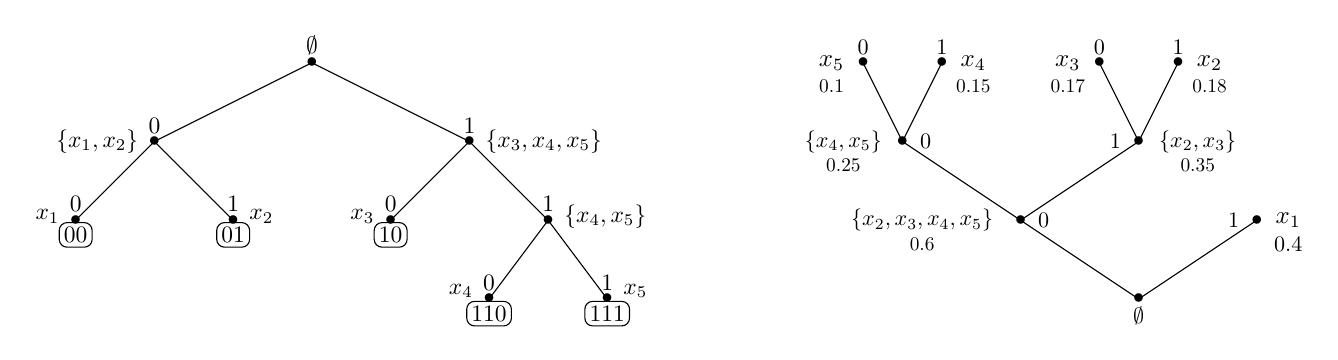
\begin{tikzpicture}%[xscale=3.5,yscale=3]
\shorthandoff{>}
%
% Codigo de Fano
\begin{scope}
\draw(0,0) node[scale=.8]{$\bullet$} node[above,scale=.85]{$\emptyset$};
%
% -----
%
\draw (0,0) -- (-2,-1) node[scale=.8]{$\bullet$} node[above,scale=.85]{$0$};
\draw (-2.1,-1) node[left,scale=.85]{$\{ x_1,x_2\}$};
%
\draw (0,0) -- (2,-1) node[scale=.8]{$\bullet$} node[above,scale=.85]{$1$};
\draw(2.1,-1) node[right,scale=.85]{$\{ x_3,x_4,x_5\}$};
%
% -----
%
\draw (-2,-1) -- (-3,-2) node[scale=.8]{$\bullet$} node[above,scale=.85]{$0$}
node[inner sep=2pt,outer sep=1pt,draw=black,below,scale=.85,rounded corners=1mm]{$00$};
\draw (-3.1,-1.95) node[left,scale=.85]{$\boldsymbol{x_1}$};
%
\draw (-2,-1) -- (-1,-2) node[scale=.8]{$\bullet$} node[above,scale=.85]{$1$}
node[inner sep=2pt,outer sep=1pt,draw=black,below,scale=.85,rounded corners=1mm]{$01$};
\draw (-.9,-1.95) node[right,scale=.85]{$\boldsymbol{x_2}$};
%
\draw (2,-1)-- (1,-2) node[scale=.8]{$\bullet$} node[above,scale=.85]{$0$}
node[inner sep=2pt,outer sep=1pt,draw=black,below,scale=.85,rounded corners=1mm]{$10$};
\draw (.9,-1.95) node[left,scale=.85]{$\boldsymbol{x_3}$};
%
\draw (2,-1)-- (3,-2) node[scale=.8]{$\bullet$} node[above,scale=.85]{$1$};
\draw (3.1,-1.95) node[right,scale=.85]{$\{ x_4 , x_5 \}$};
%
% -----
%
\draw (3,-2)-- (2.25,-3) node[scale=.8]{$\bullet$} node[above,scale=.85]{$0$}
node[inner sep=2pt,outer sep=1pt,draw=black,below,scale=.85,rounded corners=1mm]{$110$};
\draw (2.15,-2.9) node[left,scale=.85]{$\boldsymbol{x_4}$};
%
\draw (3,-2)-- (3.75,-3) node[scale=.8]{$\bullet$} node[above,scale=.85]{$1$}
node[inner sep=2pt,outer sep=1pt,draw=black,below,scale=.85,rounded corners=1mm]{$111$};
\draw (3.85,-2.9) node[right,scale=.85]{$\boldsymbol{x_5}$};
\end{scope}
%
%
% Codigo de Huffman
\begin{scope}[xshift=12cm]
\draw (-5,0) node[scale=.8]{$\bullet$} node[above,scale=.8]{$0$}
-- (-4.5,-1) node[scale=.8]{$\bullet$} node[right,scale=.8]{$\:\: 0$}
-- (-4,0) node[scale=.8]{$\bullet$} node[above,scale=.8]{$1$};
\draw(-5.4,0) node[scale=.9]{$\boldsymbol{x_5}$};
\draw(-5.4,-.3) node[scale=.7]{$0.1$};
\draw(-3.6,0) node[scale=.9]{$\boldsymbol{x_4}$};
\draw(-3.6,-.3) node[scale=.7]{$0.15$};
\draw(-5.25,-1) node[scale=.8]{$\{x_4,x_5\}$};
\draw(-5.25,-1.3) node[scale=.7]{$0.25$};
%
% -----
%
\draw (-2,0) node[scale=.8]{$\bullet$} node[above,scale=.8]{$0$}
-- (-1.5,-1) node[scale=.8]{$\bullet$} node[left,scale=.8]{$1\:\: $}
-- (-1,0) node[scale=.8]{$\bullet$} node[above,scale=.8]{$1$};
\draw(-2.4,0) node[scale=.9]{$\boldsymbol{x_3}$};
\draw(-2.4,-.3) node[scale=.7]{$0.17$};
\draw(-.6,0) node[scale=.9]{$\boldsymbol{x_2}$};
\draw(-.6,-.3) node[scale=.7]{$0.18$};
\draw(-.75,-1) node[scale=.8]{$\{x_2,x_3\}$};
\draw(-.75,-1.3) node[scale=.7]{$0.35$};
%
% -----
%
\draw (-4.5,-1) -- (-3,-2) node[scale=.8]{$\bullet$} node[right,scale=.8]{$\:\: 0$} -- (-1.5,-1);
\draw(-4.25,-2) node[scale=.8]{$\{x_2,x_3,x_4,x_5\}$};
\draw(-4.25,-2.3) node[scale=.7]{$0.6$};
%
% -----
%
\draw (-3,-2) -- (-1.5,-3) node[scale=.8]{$\bullet$} node[below,scale=.8]{$\emptyset$}
-- (0,-2) node[scale=.8]{$\bullet$} node[left,scale=.8]{$1\:\:$};
\draw(.4,-2) node[scale=.9]{$\boldsymbol{x_1}$};
\draw(.4,-2.3) node[scale=.8]{$0.4$};
\end{scope}
\end{tikzpicture} \end{center}
%
\leyenda{Construcci\'on de  un c\'odigo binario  sobre $\C =  \{0 \, , \,  1 \}$
  asociado al vector de probabilidad $p_X = \protect\begin{bmatrix} 0.4 & 0.18 &
    0.17 & 0.15 & 0.1 \protect\end{bmatrix}^t$ sobre el arbol de Kraft.  En este
  caso, $H_2(X)  \approx 2.1514$\ (a): Enfoque  de Fano, saliendo  de la ra\'iz.
  En cada nudo, se menciona el conjunto de s\'imbolos que va a tener el c\'odigo
  correspondiente  (en negro  cuando  es un  solo  s\'imbolo).  Se  pasa de  una
  profundez  a la  otra  dividiendo los  conjunto  en sub-conjuntos  a lo  m\'as
  equiprobables.   Esta construcci\'on  da el  c\'odigo \  $c^\fa(x_1) =  00, \:
  c^\fa(x_2) = 01, \: c^\fa(x_3) = 10, \: c^\fa(x_4) = 110, \: c^\fa(x_5) = 111$
  \ de  largo promedio \ $L\left(  c^\fa \right) =  2.25$.  \ \ (b):  Enfoque de
  Huffman, saliendo de las hojas.   En cada nudo, se menciona el correspondiente
  (i) conjunto de s\'imbolos,  (ii) $\cod_i$ de esta profundez/posici\'on, (iii)
  la probabilidad  asociada al  conjunto.  Se  pasa de una  profundez a  la otra
  juntando  los conjuntos  menos  probables en  sobre-conjuntos.   En negro  son
  indicados los s\'imbolos simples: van a tener el c\'odigo agregando los de los
  nudos yendo de la ra\'iz hasta  las hojas.  Esta construcci\'on da el c\'odigo
  \ $c^\huf(x_1) = 1, \: c^\huf(x_2) = 011, \: c^\huf(x_3) = 010, \: c^\huf(x_4)
  = 001, \: c^\huf(x_5) = 000$ \ de largo promedio \ $L^\opt = 2.2$.}
%
\label{Fig:SZ:FanoHuffmanCodes}
\end{figure}


Se notar\'a  de que, tratando  de una fuente  \ $\{ X_t  \}_{t \in \Zset}$  \ de
variables independientes,  se puede  codificar la fuente  con un  largo promedio
arbitrariamente cerca  de $H_d(X)$.   El principio es  de considerar  vectores \
$\begin{bmatrix} X_1 & \cdots &  X_n \end{bmatrix}^t$ \ viviendo sobre \ $\X^n$,
llamado {\it extensi\'on de orden $n$ de la fuente}, con un c\'odigo descifrable
(o libre de  prefijo) de esta extensi\'on; es llamado  {\it codificaci\'on de la
  extensi\'on  de  la  fuente}  pero  no  es  necesariamente  una  extension  de
$c$. As\'i, \ $H_d(X_1 , \ldots ,  X_n) \le L^{\opt,n} < H_d(X_1 , \ldots , X_n)
+ 1$, es decir, de la independencia,
%
\[
H_d(X)  \:  \le \:  \frac{L^{\opt,n}}{n}  \: <  \:  H_d(X)  + \frac{1}{n}  \quad
\mbox{por s\'imbolo}
\]
%
(ver  tambi\'en~\cite[cap. 13,  teorema de  Shannon]{Rio07}). Fijense  que  si \
$\displaystyle   \lim_{n   \to  \infty}   \frac{L^{\opt,n}}{n}   \to  H(X)$,   \
$\frac{L^{\opt,n}}{n}$ \ no  es necesariamente decreciente con respeto  a \ $n$.
Eso  es descrito  figura Fig.~\ref{Fig:SZ:CodigosExtensiones}.   Lo  mismo puede
ocurir  con el c\'odigo  de Shannon  y lo  de Fano.   Adem\'as, el  cardenal del
alfabeto  extendido $\X^n$  crece exponencialmente  con $n$,  lo que  no permite
elegir un $n$ muy grande.

\begin{figure}[h!]
%
\begin{center} \begin{tikzpicture}
\shorthandoff{>}
%
%Axes
%\pgfmathsetmacro{\Hd}{-.34*log2(.34)-.66*log2(.66)}; % entropia para p = [.34 .66]
%
\draw[>=stealth,->] (.9,0)--(15.5,0) node[right]{\small $n$};
\draw[>=stealth,->] (1,-.1)--(1,2.5) node[above,scale=.65]{$\displaystyle \frac{L^{\opt,n}}{n} - H_d(X)$};
\foreach \k in {1,...,15} {\draw (\k,0)--(\k,-.1) node[below,scale=.7]{\k};}
\draw (1,2)--(.9,2) node[left,scale=.7]{$1-H_d(X)$};
%
\draw[thin,color=gray!70] plot[mark=*,mark size=1.25, mark options={black}] file {Data/Loptn_p033_libro.txt};
%\draw[thin,dashed] (-.1,\dec) node[left]{\small $H_d(X)$} --(12,\dec);
%\draw[thin,dashed] plot [domain=2:13,samples=100] (\x,{50/\x});
% ATTENTION, trace de (L-Hd) normalise puis double pour une question de lisibilite
\end{tikzpicture}
 \end{center}
%
\leyenda{$\frac{L^{\opt,n}}{n}-H_d(X)$  (puntos),   diferencia  entre  el  largo
  promedio \'optimo por s\'imbolo de las  extensiones \ $\X^n$ \ de orden $n$ de
  la fuente $\X$ y la cota inferior en funci\'on de $n$. La linea llena en grise
  sirve como gu\'ia. En esta ilustraci\'on se usa el ejemplo lo m\'as simple con
  \   $d   =   2$  \   y   \   $p   =   \protect\begin{bmatrix}  0.33   &   0.67
    \protect\end{bmatrix}^t$.}
%
\label{Fig:SZ:CodigosExtensiones}
\end{figure}

\

Para  codificar una  fuente, que  se haga  el c\'odigo  \'optimo de  Fano,  o de
Shannon,  hace  falta  usar  la  distribuci\'on de  probabilidad  de  la  fuente
$X$. Pr\'acticamente, es usual que no se la tiene. Frecuentemente, es estimada a
partir de datos,  o, dicho de otra manera, se  c\'odifica con una distribuci\'on
que no es la distribuci\'on verdadera de la fuenta. Una pregunta que surge es de
conocer lo que se pierde usando una distribuci\'on no adaptada (o ``falsa''). La
respuesta general  no es obvia, pero  tratando del c\'odigo de  Shannon se puede
contestar:

\begin{teorema}[C\'odigo falso de Shannon]
\label{Teo:SZ:CodigoFalsoShannon}
%
Sea $c^\sh(p)$  el c\'odigo  de Shannon sobre  el alfabeto  c\'odigo \ $\C  = \{
\cod_1 \, , \, \ldots \, ,  \, \cod_d \}$ asociado a la distribuci\'on $p$.  Sea
$X$  \  fuente  sobre  \  $\X$,  de  distribuci\'on  \  $p_X$  \  y  \  $q$  una
distribuci\'on cualquiera (ej.   estimada de $p_X$ presupuesta\ldots).  Entonces
el largo promedio  \ $L_{c^\sh(q)}$ \ del c\'odigo \ $c^\sh(q)$  \ aplicado a la
fuente \ $X$ \ satisface las desigualdades siguientes
  %
  \[
  H_d(p_X) +  D_{\mathrm{kl},d}\left( \left.  p_X \right\| q  \right) \:  \le \:
  L_{c^\sh(q)} \: < \: H_d(p_X)  + D_{\mathrm{kl},d}\left( \left. p_X \right\| q
  \right) + 1.
  \]
\end{teorema}
%
\begin{proof}
  Por definici\'on,
  \[
  L_{c^\sh}(q) = \sum_{x \in X} p_X(x) \, \Big\lceil\! -\log_d q(x) \Big\rceil.
  \]
  %
  La desigualdad viene de  \ $a \le \lceil a \rceil < a +  1$ \ y escribiendo $-
  p_X \log_d q = - p_X \log_d p_X + p_X \log \left( \frac{p_X}{q} \right)$.
\end{proof}
%
Olvidando el  posible extra dit (pensar  a la c\'odification  por bloques), este
teorema  da  una  interpretaci\'on  operacional  a  la  entrop\'ia  relativa,  o
divergencia  de  Kullback-Leibler.   Esta  cantidad  cuantifica  la  perdida  en
t\'ermino de largo  promedio codificando con una distribuci\'on  falsa. Dicho de
otra manera,  usando $q$  en lugar de  $p_X$, se  usa la informaci\'on  de $p_X$
porque se  c\'odifica la fuente $X$,  pero suponiendo la  distribuc\'ion $q$, se
piedre lo  que representa la  informaci\'on relativa de  $p_X$ con respeto  a la
referencia (distribuci\'on supuesta) $q$.

\

Existen varios otros  modos de codificar s\'imbolos. En  particular, con la meta
de transmitir los s\'imbolos codificados  en un canal de comunicaci\'on, a veces
no  es oportuno  de compresar  drasticamente  el mensaje.   Existen por  ejemplo
codificaciones que permiten una correcci\'on  de error en la recepci\'on. Pueden
tomar  en  cuenta  las  caracter\'isticas  del canal  de  transmisi\'on.   Estas
consideraciones  van m\'as  all\'a de  la ilustraci\'on  de esta  secci\'on.  El
lector puede referirse a~\cite{Ber74, Gal78, Say03, CovTho06, Rio07} entre otros
para tener m\'as detalles sobre varios esquemas de codificaci\'on/compresi\'on.

% R.  M.  Fano.  Class  notes  for Transmission  of  Information,  course  6.574
% (Technical Report). MIT, Cambridge, MA, 1952

%\SZ{Dire  un mot  sur  le codage  canal.   Cf avec  la  distribucion optimale  /
%  capacite cf. Elias 1954 - error free coding, Elias 1955 - error noisy channel,
%  Elias 57  - list  for decoding noisy  channels, Berlekamp (serie  papiers cles
%  dans les premiers).}

% ================================= Gaz perfecto

\subseccion{Gas perfecto}
\label{Ssec:SZ:GasPerfecto}

En el marco del gas perfecto

\SZ{Va donner un lien avec Boltzmann}


\

\SZ{Feder  Merhav  IT'94  et  lien  avec  discrimination;  Vacisek  en  test  de
  Gaussianite et cf plus loin avec generalises Gok75 etc}


% ============================== Generalizadas================================ %


\seccion{Entropias y divergencias generalizadas}
\label{sec:SZ:Generalizadas}

A pesar de que la entropia de Shannon y sus cantidades asociadas demostraron sus
potencias tan de un punto de vista descriptivo que en termino de aplicaciones en
la  transmisi\'on  de  la  informaci\'on  y  la  compresi\'on,  varios  nociones
informacionales, de  tipo entropias o  divergencias, aparecieron luego.  En esta
secci\'on no se  desarollar\'a todos los enfoques ni  todas las aplicaciones tan
la  literatura es  importante. La  meta  es dar  los caminos  conduciendo a  las
generalizaciones de la  entropia de Shannon por un lado, y  de la divergencia de
Kullback-Leibler por el otro lado. No son siempre vinculados, a pesar de que sea
desirable que a cada entropia sean asociados nociones de entropias condicionales
y relativas.

% ================================= Salicru

\subseccion{Entropias y propiedades}
\label{sec:SZ:Salicru}

Si  la entropia  de  Shannon  fue el  punto  de salida  fundamental  en todo  el
desarollo de la teoria de la informaci\'on, un poco mas de una decada despues de
su    papel   clave    y   muy    completo,   R\'enyi    propuso    una   medida
generalizada~\cite{Ren61}. Su  punto de  vista fue mas  matematico que  fisico o
ingeniero.  Retom\'o los axiomas de Fadeev~\cite{Fad56, Fad58, Khi57}
% Feinstein, cf ref  de R�nyi
%
a  probabilidades  incompletas   $p  =  \begin{bmatrix}  p_1  &   \cdots  &  p_n
\end{bmatrix}^t,  \quad p_i  \ge  0,  \quad w_p  =  \sum_i p_i  \le  1$: (i)  la
invarianza de  $H(p)$ por permutaci\'on de  os $p_i$, (ii) la  continuidad de la
incerteza elemental  $H(p_i)$ ($p_i$ visto como  probabilidad incompleta), (iii)
$H\left( \frac12 \right) = 1 $,  (iv) la aditividad $H(p \otimes q) = H(p)+H(q)$
donde $p \otimes q$ es el producto de Kronecker~\footnote{$\begin{bmatrix} p_1 &
\cdots & p_n \end{bmatrix}^t \otimes \begin{bmatrix} q_1 & \cdots & q_m
\end{bmatrix}^t = \begin{bmatrix} p_1 q_1 & \cdots  & p_1 q_m & \cdots & p_n q_1
&  \cdots  &  p_n  q_m  \end{bmatrix}^t$.}, \ie  probabilidad  conjunta  de  dos
variables independientes,  y consider\'o en  lugar de la recursividad  un axioma
dicho de valor promedio,  axioma muy parecido a la recursividad. Para  $p$ \ y \
$q$ probabilidades incompletas tales que $p \, \cup \, q = \begin{bmatrix} p_1 &
\cdots & p_n  & q_1 & \cdots  & q_m \end{bmatrix}^t$ sea incompleta  ($w_p + w_q
\le 1$),  el axioma  (v) es  $H(p \, \cup  \, q)  = \frac{w_p \,  H(p) +  w_q \,
H(q)}{w_p  + w_q}$.   Demostr\'o que  con (v)  en lugar  de la  recursividad, el
conjunto  de   axiomas  conduce  de  nuevo   a  la  entropia   de  Shannon.   La
generalizaci\'on  propuesta  por  R\'enyi  era  de  generalizar  el  axioma  (v)
remplazando la media  aritm\'etico por una media generalizada  (v') $H^\ren(p \,
\cup \, q) =  g^{-1} \left( \frac{w_p \, g\big( H^\ren(p) \big)  + w_q \, g\big(
H^\ren(q) \big)}{w_p  + w_q}\right)$ con $g$ estrictamente  monotona y continua,
llamado media {\it cuasi-aritm\'etica,  o quasi-lineal, o de Kolmogorov-Nagumo}.
De  las  propiedades de  la  media  cuasi-aritmetica~\cite{Nag30, Kol30,  Kol91,
HarLit52}, eso  es equivalente a  buscar una entropia elemental  $H^\ren(p_i)$ y
remplazar  la media  aritm\'etica  $\sum_i  p_i H^\ren(p_i)$  por  una media  de
Kolmogorov-Nagumo, $g^{-1} \left( \sum_i  p_i g\big( H^\ren(p_i) \big) \right)$.
R\'enyi propus\'o la funci\'on de Kolmogorov-Nagumo $g_\alpha(x) = 2^{(\alpha-1)
x},  \quad \alpha >0,  \quad \alpha  \ne 1$,  probando que  la entropia  que los
axiomas (i)-(ii)-(iii)-(iv)-(v') se  cumplen y conduce a la  entropia de R\'enyi
de un vector de probabilidad $p$,
%
\[
H_\alpha^\ren(p) = \frac{1}{1-\alpha} \log_2 \left( \sum_{i=1}^n p_i^\alpha \right)
\]
%
\noindent   Relaxando  el  axioma   (iii),  se   puede  elegir   $g_\alpha(x)  =
a^{(\alpha-1) x}, \quad  a > 0, \quad a  \ne 1$; el logaritmo ser\'a  de la base
$a$ cualquiera; En  lo que sigue, usaremog $\log$ sin  precisar la elecci\'on de
base.   R\'enyi  nombr\'o  esta  medida  de incerteza  {\it  entropia  de  orden
$\alpha$}. Notablemente,
%
\[
H_1^\ren(p)  \equiv   \lim_{\alpha  \to   1}  H_\alpha^\ren(p)   =   H(p)  \quad
\mbox{entropia de Shannon}
\]
%
\noindent En otros  terminos, la clase de R\'enyi  contiene como caso particular
la  entropia  de  Shannon.  En  su  papel,  R\'enyi  introdujo una  ganancia  de
informaci\'on,  parecida  a  una  entropia  relativa,  probando  que  las  solas
entropias admisibles  son la  de Shannon  y la que  introdujo. Volveremos  en la
secci\'on  siguiente sobre  esta entropia  relativa, o  divergencia  de R\'enyi.
\SZ{Preciser les quelques  proprietes qui se conservent, dont  la concavite pour
$\alpha \le 1$.}

Unos a\~nos despu\'es de R\'enyi, de la famosa escuela matematica \SZ{checa}, J.
Havrda \& F.  Charv\'at en~\cite{HavCha67} volvieron a los axiomas de Khintchin,
para  extender la entopia  de Shannon,  \ie considerando  (i) la  invarianza por
permutaci\'on, (ii) la continuidad, (iii) la expensividad, (iv) $H^\hc(1) = 0$ y
$H^\hc\left( \frac12 , \frac12 \right)  = 1$, pero generalisando la recursividad
por (v) $H^\hc(p_1,\ldots,p_n)  = H^\hc(p_1,\ldots,p_{n-2},p_{n-1}+p_n) + \alpha
(p_{n-1}+p_n)^\alpha         H^\hc\left(         \frac{p_{n-1}}{p_{n-1}        +
p_p},\frac{p_n}{p_{n-1}  +  p_p} \right),  \quad  \alpha  > 0$~\footnote{En  sus
papel, lo imponen  para cualquier pars $p_i, p_j$ sin  imponer la invarianza por
permutaci\'on,  pero es  equivalente a  la exposici\'on  de este  parafo.}.  Con
$\alpha = 1$  se recupera la recursividad estandar, pero con  $\alpha \ne 1$ eso
permite  dar  un   peso  diferente  a  la  incerteza   del  estado  interno  \ie
probabilidades  que  se juntan  (la  describen  como clasificaci\'on  refinada).
Estos axiomas conducen necesariamente a la entropia (teorema~1)
%
\[
H_\alpha^\hc(p) = \frac{1}{1-2^{1-\alpha}} \left( 1 - \sum_i p_i^\alpha \right)
\]
%
que nombraron {\it $\alpha$-entropia structural}.  De nuevo, relaxando el axioma
(iv),  se puede  remplazar en  el coeficient  $2^{1-\alpha}$  por $a^{1-\alpha},
\quad a >  0, \quad a \ne 1$. De  nuevo, parae que la entropia  de Shannon es un
caso particular,
%
\[
H_1^\hc(p)  \equiv   \lim_{\alpha  \to   1}  H_\alpha^\hc(p)   =   H(p)  \quad
\mbox{entropia de Shannon}
\]
%
Luego, proban que $H_\alpha^\hc(p)$ es concava  con respeto a los $p_i$ y maxima
para una  distribuci\'on uniforma  (teorema~2). Aun que  no aparece as\'i  en el
papel, satisface  la propiedad de  Schur-concavidad (teorema~3). A pesar  de que
mencionan que $H_\alpha^\hc$ sea  diferente que $H_\alpha^\ren$, es sencillo ver
que hay un mapa uno-uno entre las dos entropias.

Independiente de  Havrda \&  Charv\'at, todav\'ia en  la escuela  \SZ{checa}, Z.
Dar\'oczy  en~\cite{Dar70}  defino  la  entropia  $H^f$ a  partir  de  una  {\it
funci\'on   informaci\'on}   $f$   satifaciendo   (i)  $f(0)   =   f(1)$,   (ii)
$f\left(\frac12\right)  = 1$  \ y  la ecuaci\'on  funcional (ii)  $f(x)  + (1-x)
f\left(  \frac{y}{1-x} \right)  = f(y)  + (1-y)  f\left(  \frac{x}{1-y} \right)$
sobre  $\{  (x,y)  \in [0  ;  1)^2,  \quad  x+y  \le  1 \}$,  siendo  $H^f(p)  =
\sum_{i=2}^n s_i  f\left( \frac{p_i}{s_i} \right), \quad  s_i = \sum_{j=1}^{i-1}
p_j$.   Dar\'oczy mostr\'o  que  si $f$  es medible,  o  continua en  $0$, o  no
negatiba  y  acotada, necesariamente  $f(x)  =  h_2(x) =  -x  \log_2  x -  (1-x)
\log_2(1-x)$,   conduciendo   a  la   entropia   de   Shannon  (teorema~1;   ver
tambi\'en~\cite{Lee64, Tve58}). En otros  terminos, su axioma (v) es alternativa
a la recursividad.  Para extender  la entropia de Shannon, propuso extender este
axioma   (v)   por  la   ecuaci\'on   funcional   $f_\alpha(x)  +   (1-x)^\alpha
f_\alpha\left( \frac{y}{1-x} \right) = f_\alpha(y) + (1-y)^\alpha f_\alpha\left(
\frac{x}{1-y} \right)$, lo que  condujo necesariamente a la entropia (teoremas~2
y~3)
%
\[
H_\alpha^\dar(p) = \frac{1}{1-2^{1-\alpha}} \left( 1 - \sum_i p_i^\alpha \right)
\]
%
\noindent  es  decir  nada  mas  que  la  entropia  introducida  por  Havdra  \&
Charv\'at. Sin  embargo, el  estudio de  Dar\'oczy fue mas  intensivo que  el de
Havdra  \&  Charv\'at.  Primero,  not\'o  el  mapa entre  su  entropia  y la  de
R\'enty. Luego, prob\'o que se  conserva la invarianza por permutaci\'on (no era
un  axioma), $H_\alpha^\dar\left(  \frac12  ,  \frac12 \right)  =  1$ (lo  llama
normalizaci\'on), la  expansividad, una additividad  extendida, una recursividad
extendida  precisamente  del modelo  de  Havrda-Charv\'at (teorema~4).   Prob\'o
tambi\'en  que $H_\alpha^\dar  \ge 0$  (alcanzado en  el caso  deterministico) y
m\'axima    en    el   caso    uniforme    (teorema~6),   que    incidentalmente
$H_\alpha^\dar\left(  \frac1d ,  \ldots ,  \frac1d \right)$  crece con  $d$. Muy
interesante tambi\'en es  se puede definir una entropia  condicional en el mismo
modelo  que  en   el  caso  de  Shannon  $H_\alpha^\dar(X|Y)   =  \sum_y  \left[
p_{X|Y}(x,y) \right]^\alpha  H_\alpha^\dar( p_{X|Y}(\cdot,y) )$,  que existe una
regla de cadena, $H_\alpha^\dar(X,Y)  = H_\alpha^\dar(Y) + H_\alpha^\dar(X|Y)$ y
que  condicionar reduce  la entropia  $H_\alpha^\dar(X|Y)  \le H_\alpha^\dar(X)$
(teorema~8). Mostr\'o tambi\'en que si  se pierde la additividad, se obiene para
\ $X$  \ e  \ $Y$  \ independientes \  $H_\alpha^\dar(X,Y) =  H_\alpha^\dar(X) +
H_\alpha^\dar(Y)   +   \left(   2^{1-\alpha}   -  1   \right)   H_\alpha^\dar(X)
H_\alpha^\dar(Y)$. La propiedades de regla  de cadena le permiti\'o revisitar la
caracterisaci\'on de un  canal de transmisi\'on y redefinir  una capacidad canal
extendidas (capacidad  tipo $\alpha$;  basicamente se usa  el mismo  enfoque que
Shannon,  pero usando  $H_\alpha^\dar$ en  lugar  de $H$,  ver secci\'on~6  del
papel).


\SZ{redecouverte Tsallis 1988..., Lindhardt \& Nielsen Studies in Dynamical
Systems Kongelige Danske Videnskabernes Selskab, 38(9):1-42, 1971, De nombreuses
autres, Varama 66, mais premier pas unifie Burbea-Rao; puis Salicru\newline proprietes et voir conditionnelle... moyenne adqueate}


\SZ{versiones dferenciales poner  ac\'a la  codificaci\'on  a la  Renyi, y  la
  cuantificacion fina; EPI generalizada  por Madiman, etc. Lutwak, Bercher etc.,
  Kagan}

{\bf Revisite capacite a la Daroczy?}

% ================================= Salicru

\subseccion{Divergencias y propiedades}
\label{sec:SZ:Czizar}

{\bf Extension a la Renyi, a la HC/D/T, Cressie Reads, Cressie Pardo, Vajda; cf Burbea Rao: generalization  Czizar et voir avec h phi avant meme Salicru. Cf aussi Bregmann}


% =============================== Cuanticas ================================== %


\seccion{Entropias cuanticas discretas}
\label{sec:SZ:Cuanticas}

{\bf Mas alla caso de informaciones a partir de medida; caso infinito, continuo queda en discusiones}
